\cleardoublepage
\appendix
\chapter{Manual de usuario}
\label{app:manual}

Una vez que el usuario se instale la aplicación y acceda a ella aparece en la pantalla de \textbf{inicio} Figura~\ref{fig:start}. Desde ella podrá registrarse o iniciar sesión en la aplicación.

\begin{figure}[H]
\centering
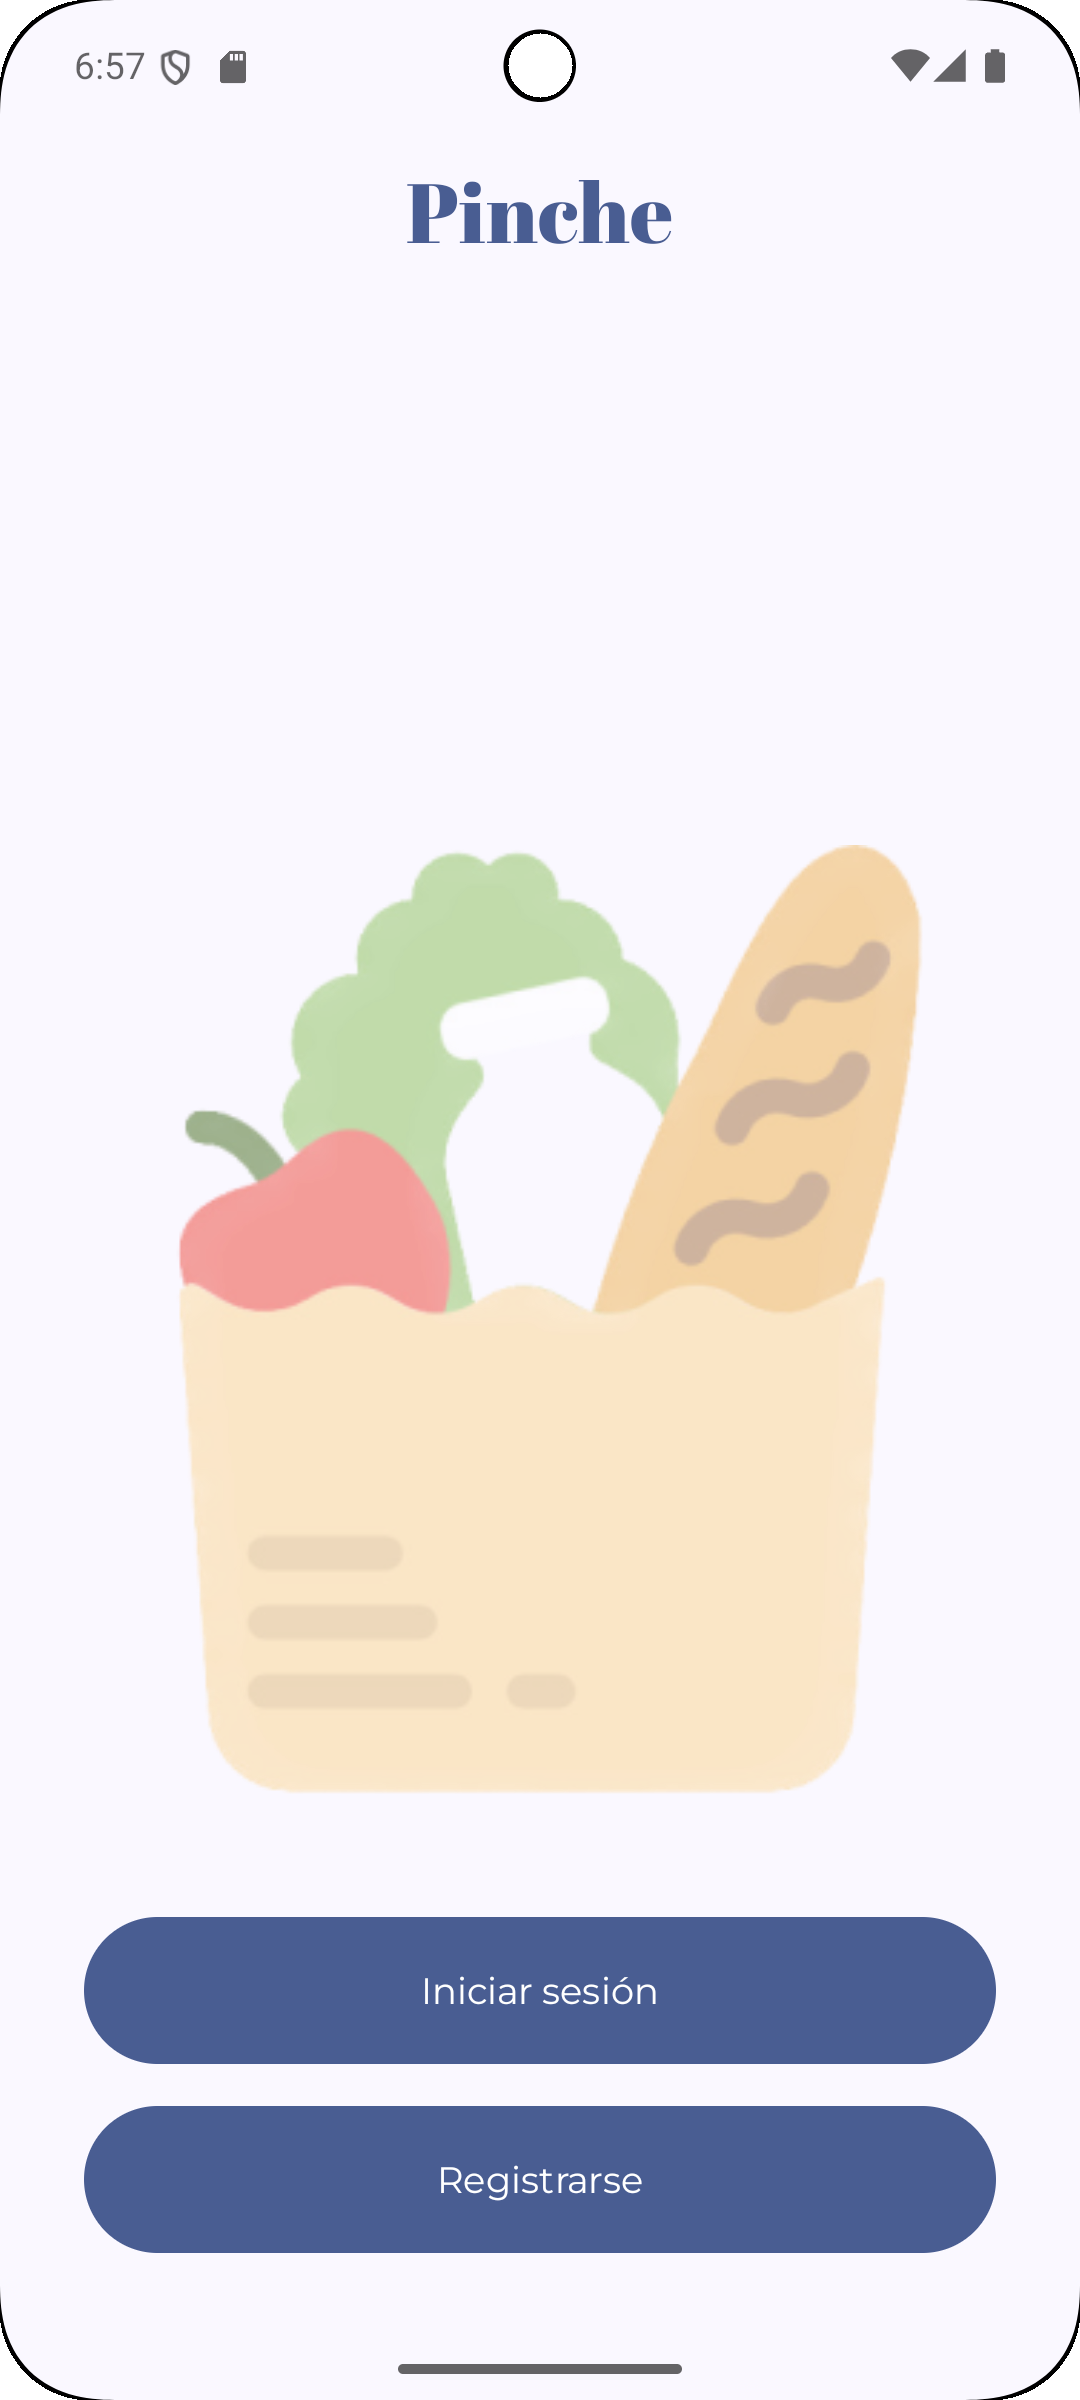
\includegraphics[width=0.32\textwidth]{./img/manual/pinche_first_screen.png}
\caption{Pantalla de inicio de Pinche}
\label{fig:start}
\end{figure}

\clearpage
%% registro
Si el usuario hace clic en registrarse, se mostrará la pantalla de \textbf{registro} Figura~\ref{fig:register-main}. Para el registro hay ciertos campos que el usuario deberá rellenar obligatoriamente Figura~\ref{fig:register-must}. Si el registro se realiza con éxito el usuario accede a la pantalla principal de la aplicación. Si no, se muestra un error Figura~\ref{fig:register-error}.

\begin{figure}[H]
    \centering

    \begin{subfigure}[b]{0.3\textwidth}
      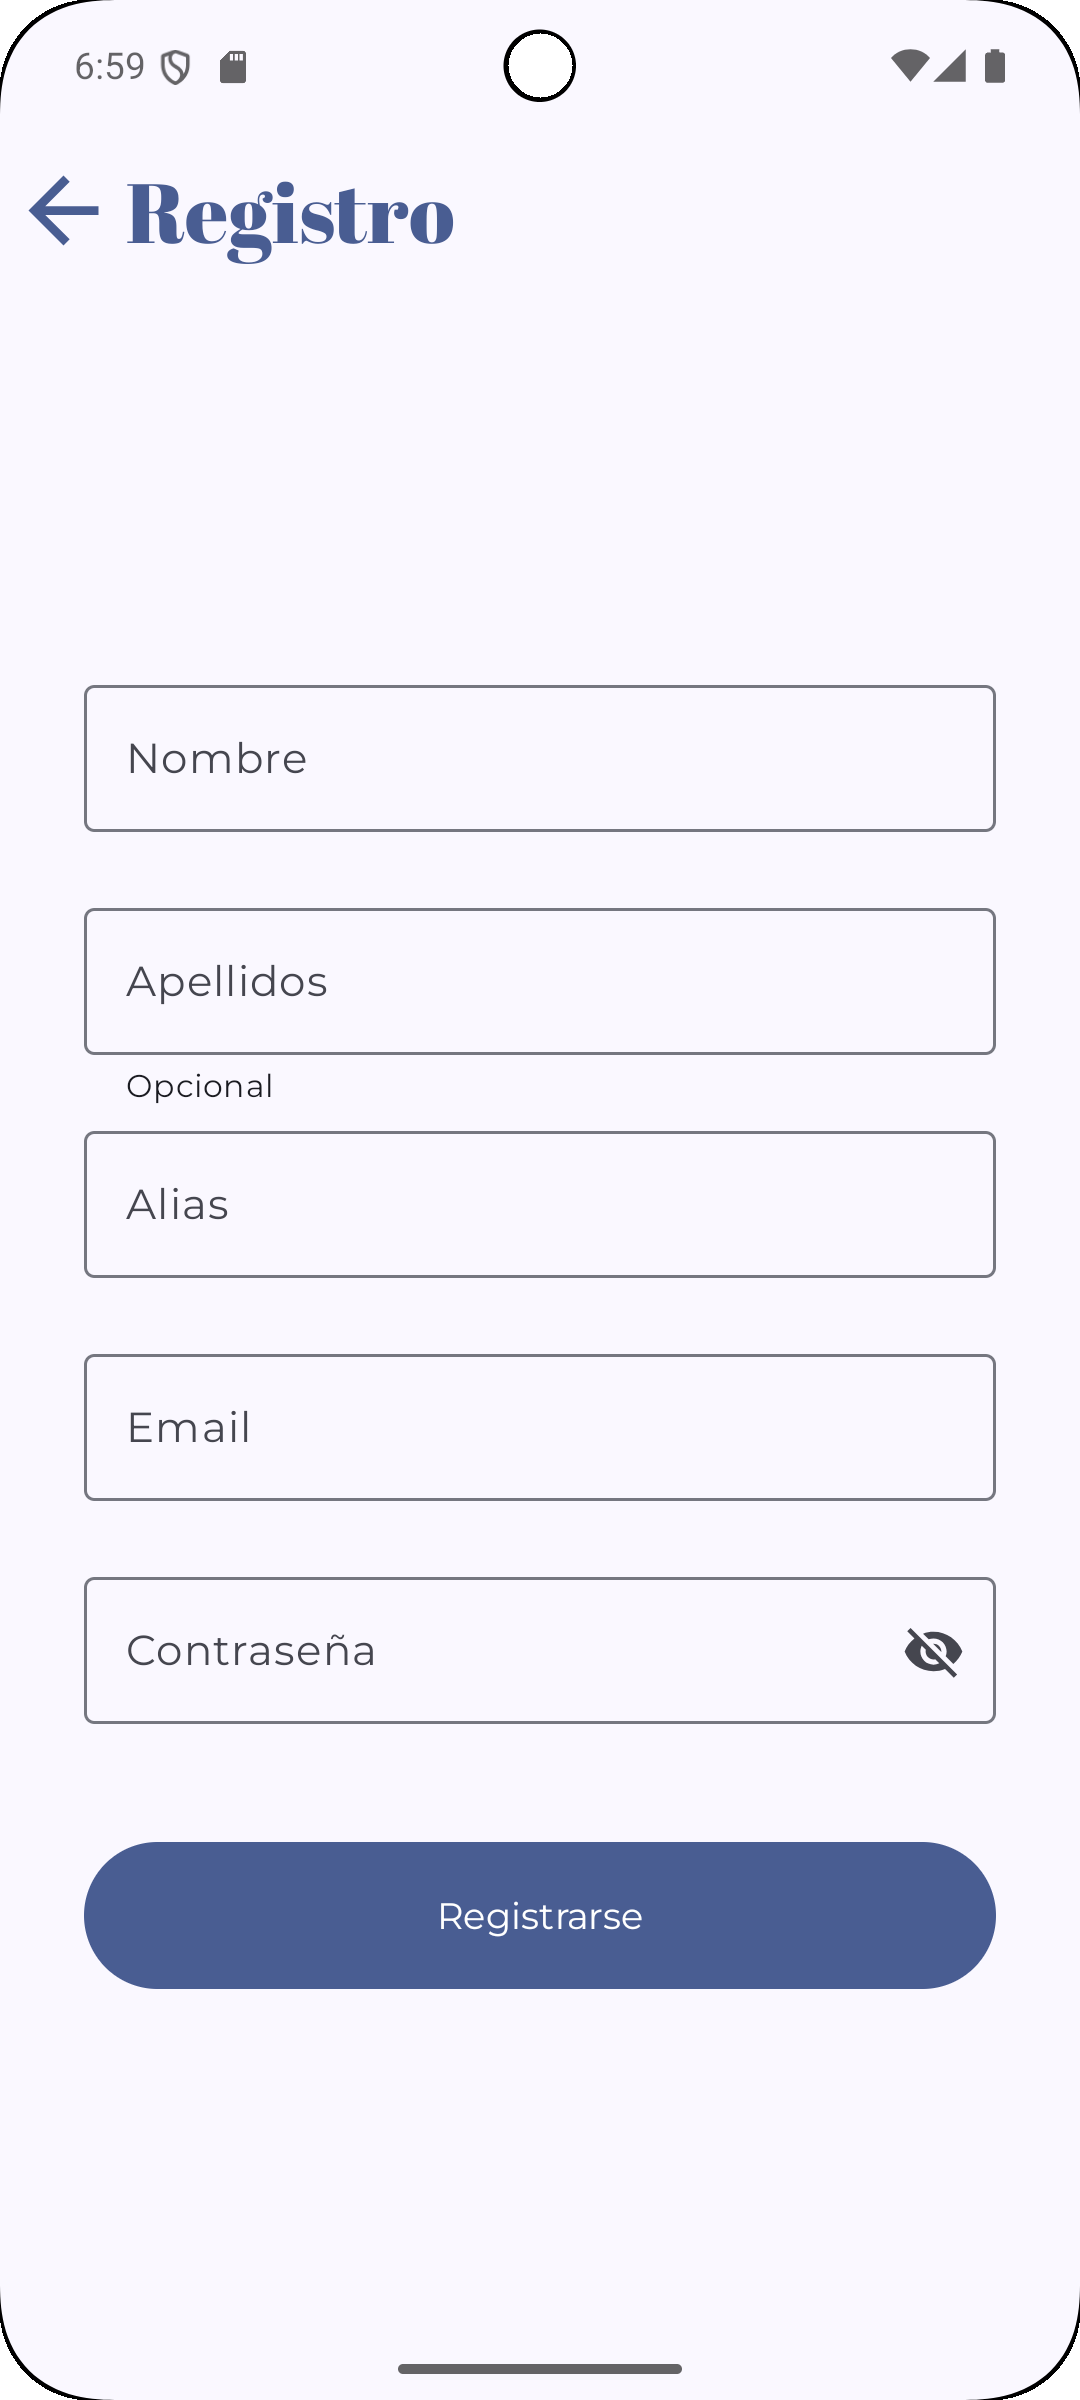
\includegraphics[width=\textwidth]{./img/manual/pinche_register.png}
      \caption{Pantalla de registro de un usuario}
      \label{fig:register-main}
    \end{subfigure}
    \hfill
    \begin{subfigure}[b]{0.3\textwidth}
      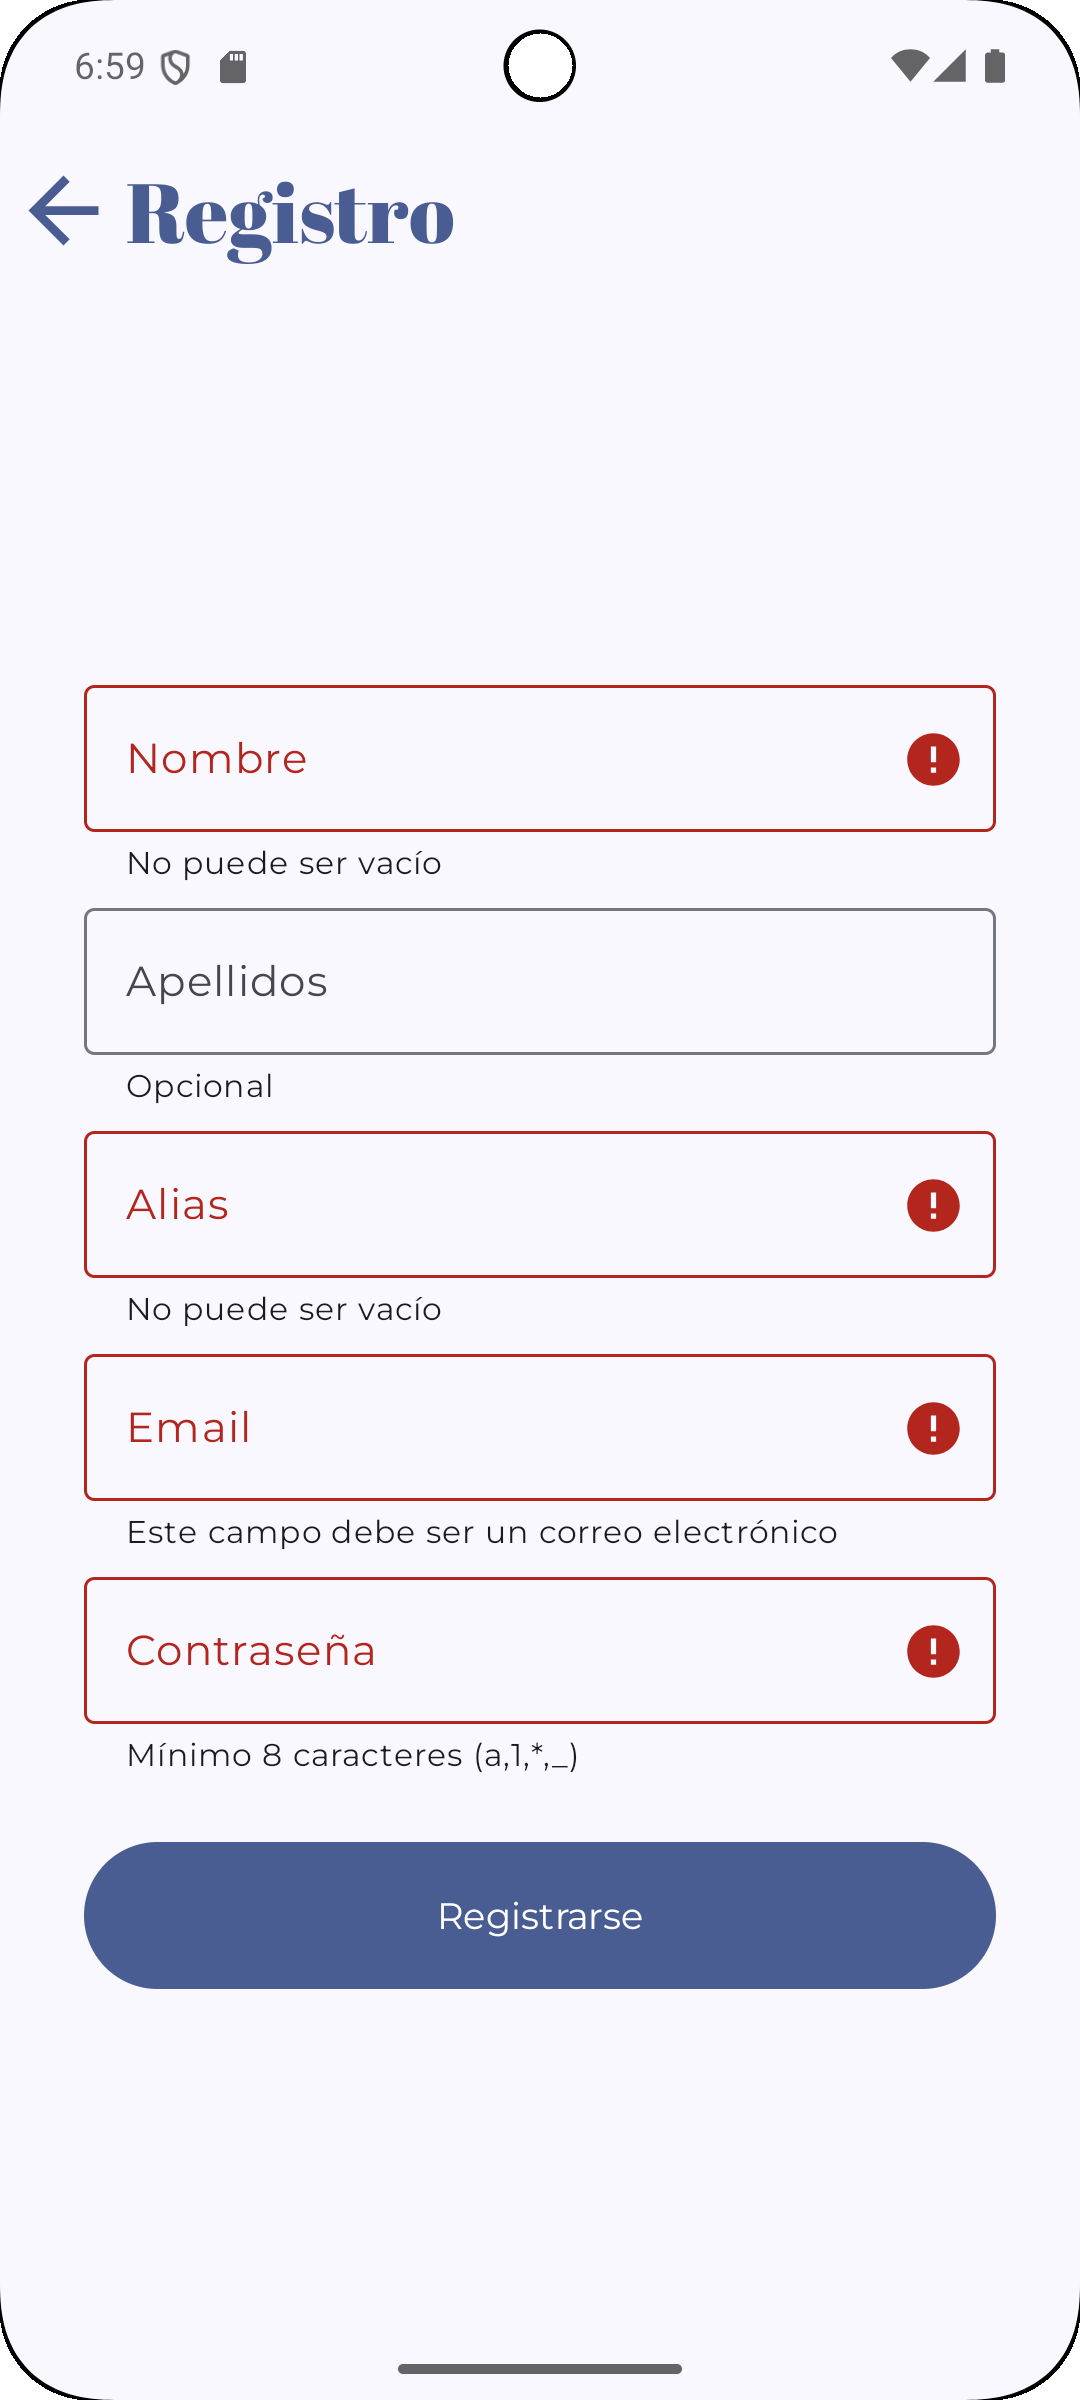
\includegraphics[width=\textwidth]{./img/manual/pinche_register_empty.png}
      \caption{Campos obligatorios en la pantalla de registro}
      \label{fig:register-must}
    \end{subfigure}
    \hfill
    \begin{subfigure}[b]{0.3\textwidth}
      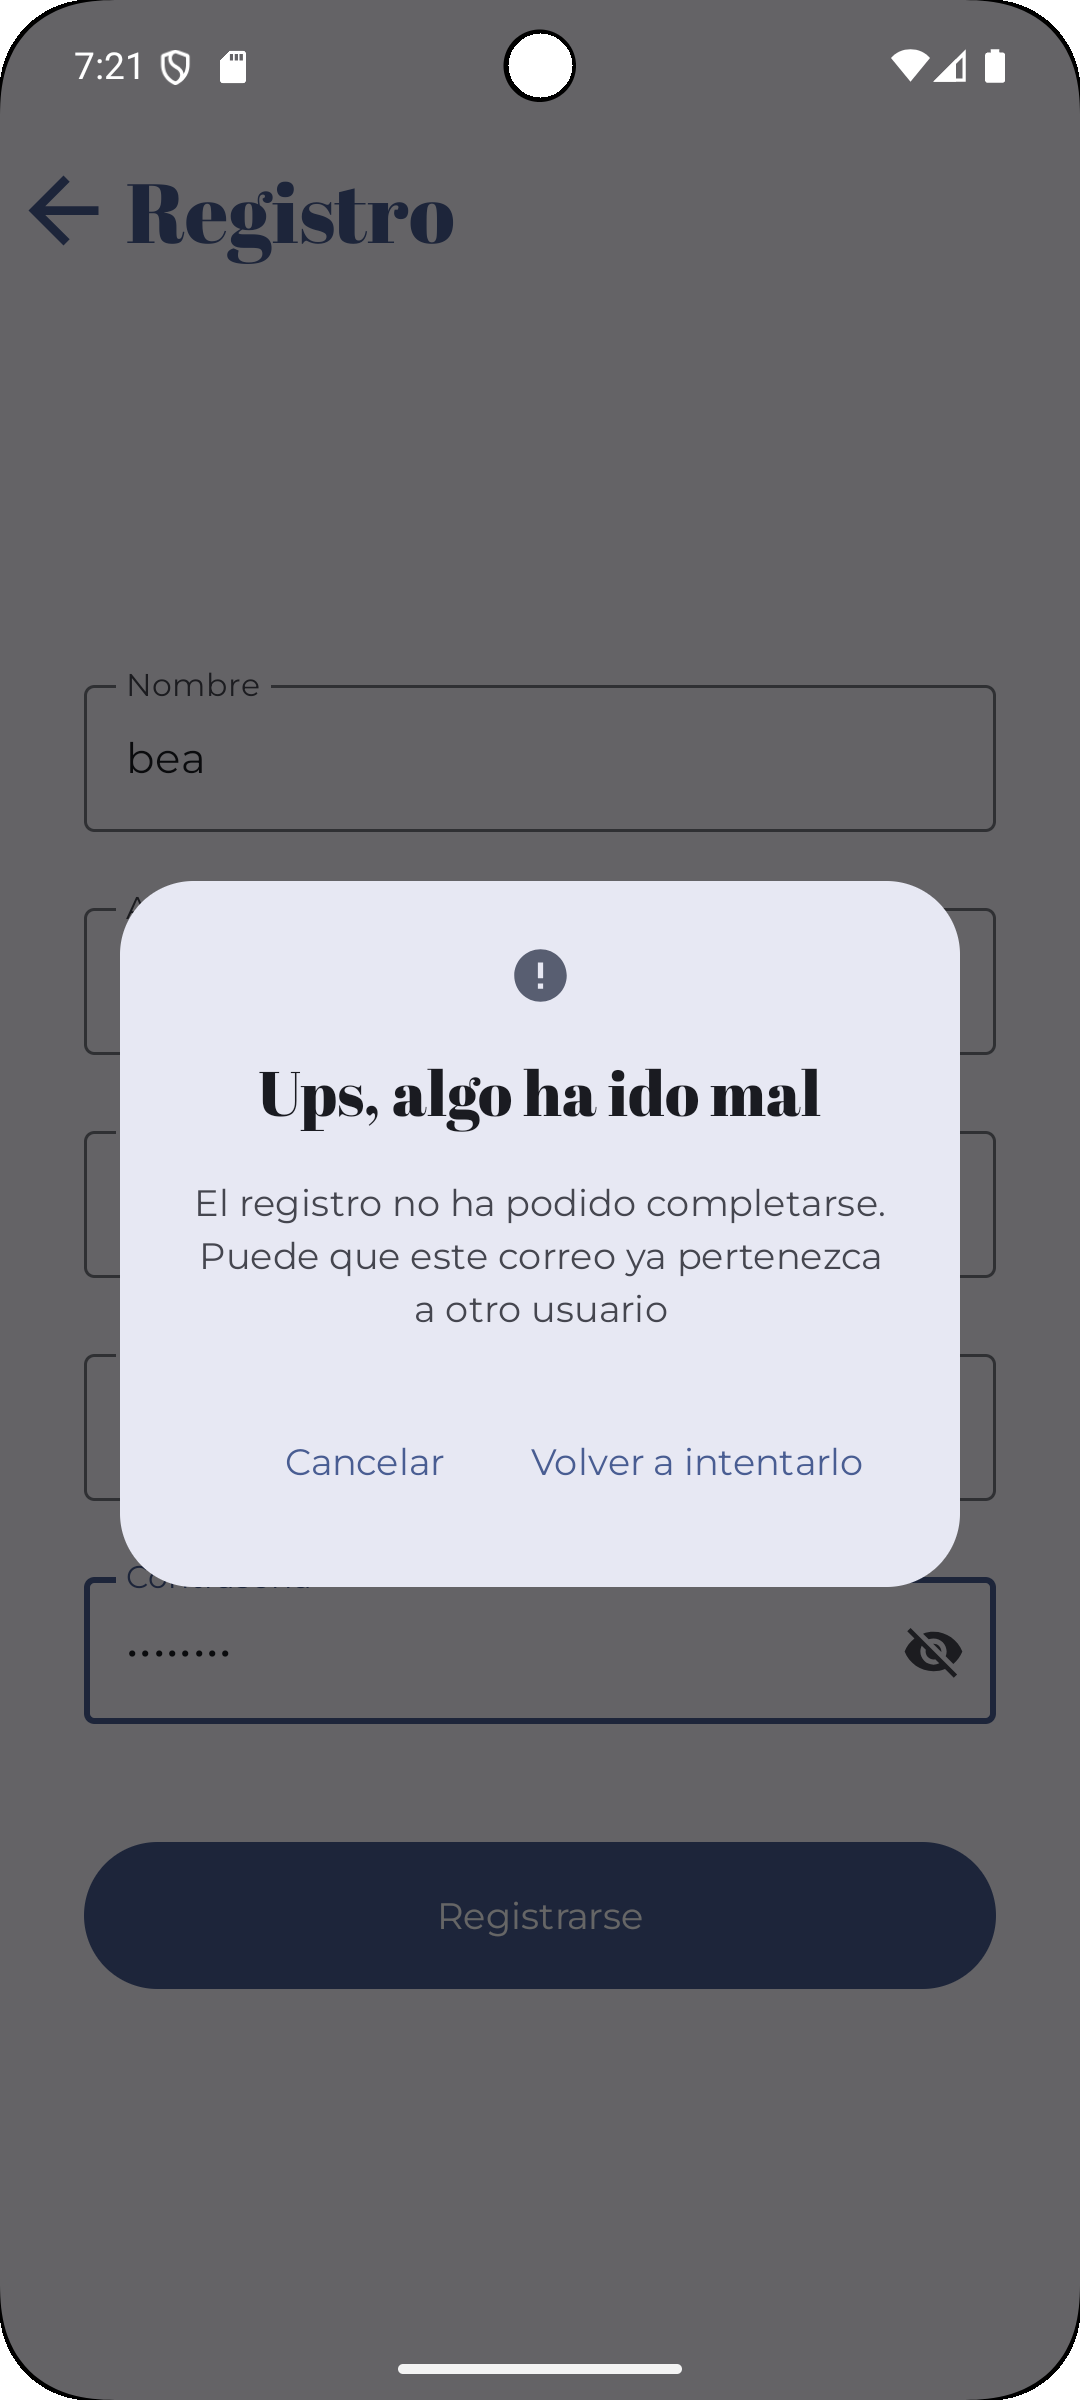
\includegraphics[width=\textwidth]{./img/manual/register_error.png}
      \caption{Mensaje de error si falla el registro de un usuario}
      \label{fig:register-error}
    \end{subfigure}

    \caption{Registro}
    \label{fig:register}
\end{figure}

%% login
\clearpage
Si el usuario ya tiene cuenta en la aplicación y accede al \textbf{inicio de sesión} se mostrará la pantalla que se muestra en la Figura~\ref{fig:login-main}. Ambos campos son obligatorios, Figura~\ref{fig:login-must}. En caso de que el inicio de sesión falle, se muestra el siguiente mensaje de error Figura~\ref{fig:login-error}.

\begin{figure}[H]
    \centering

    \begin{subfigure}[b]{0.3\textwidth}
      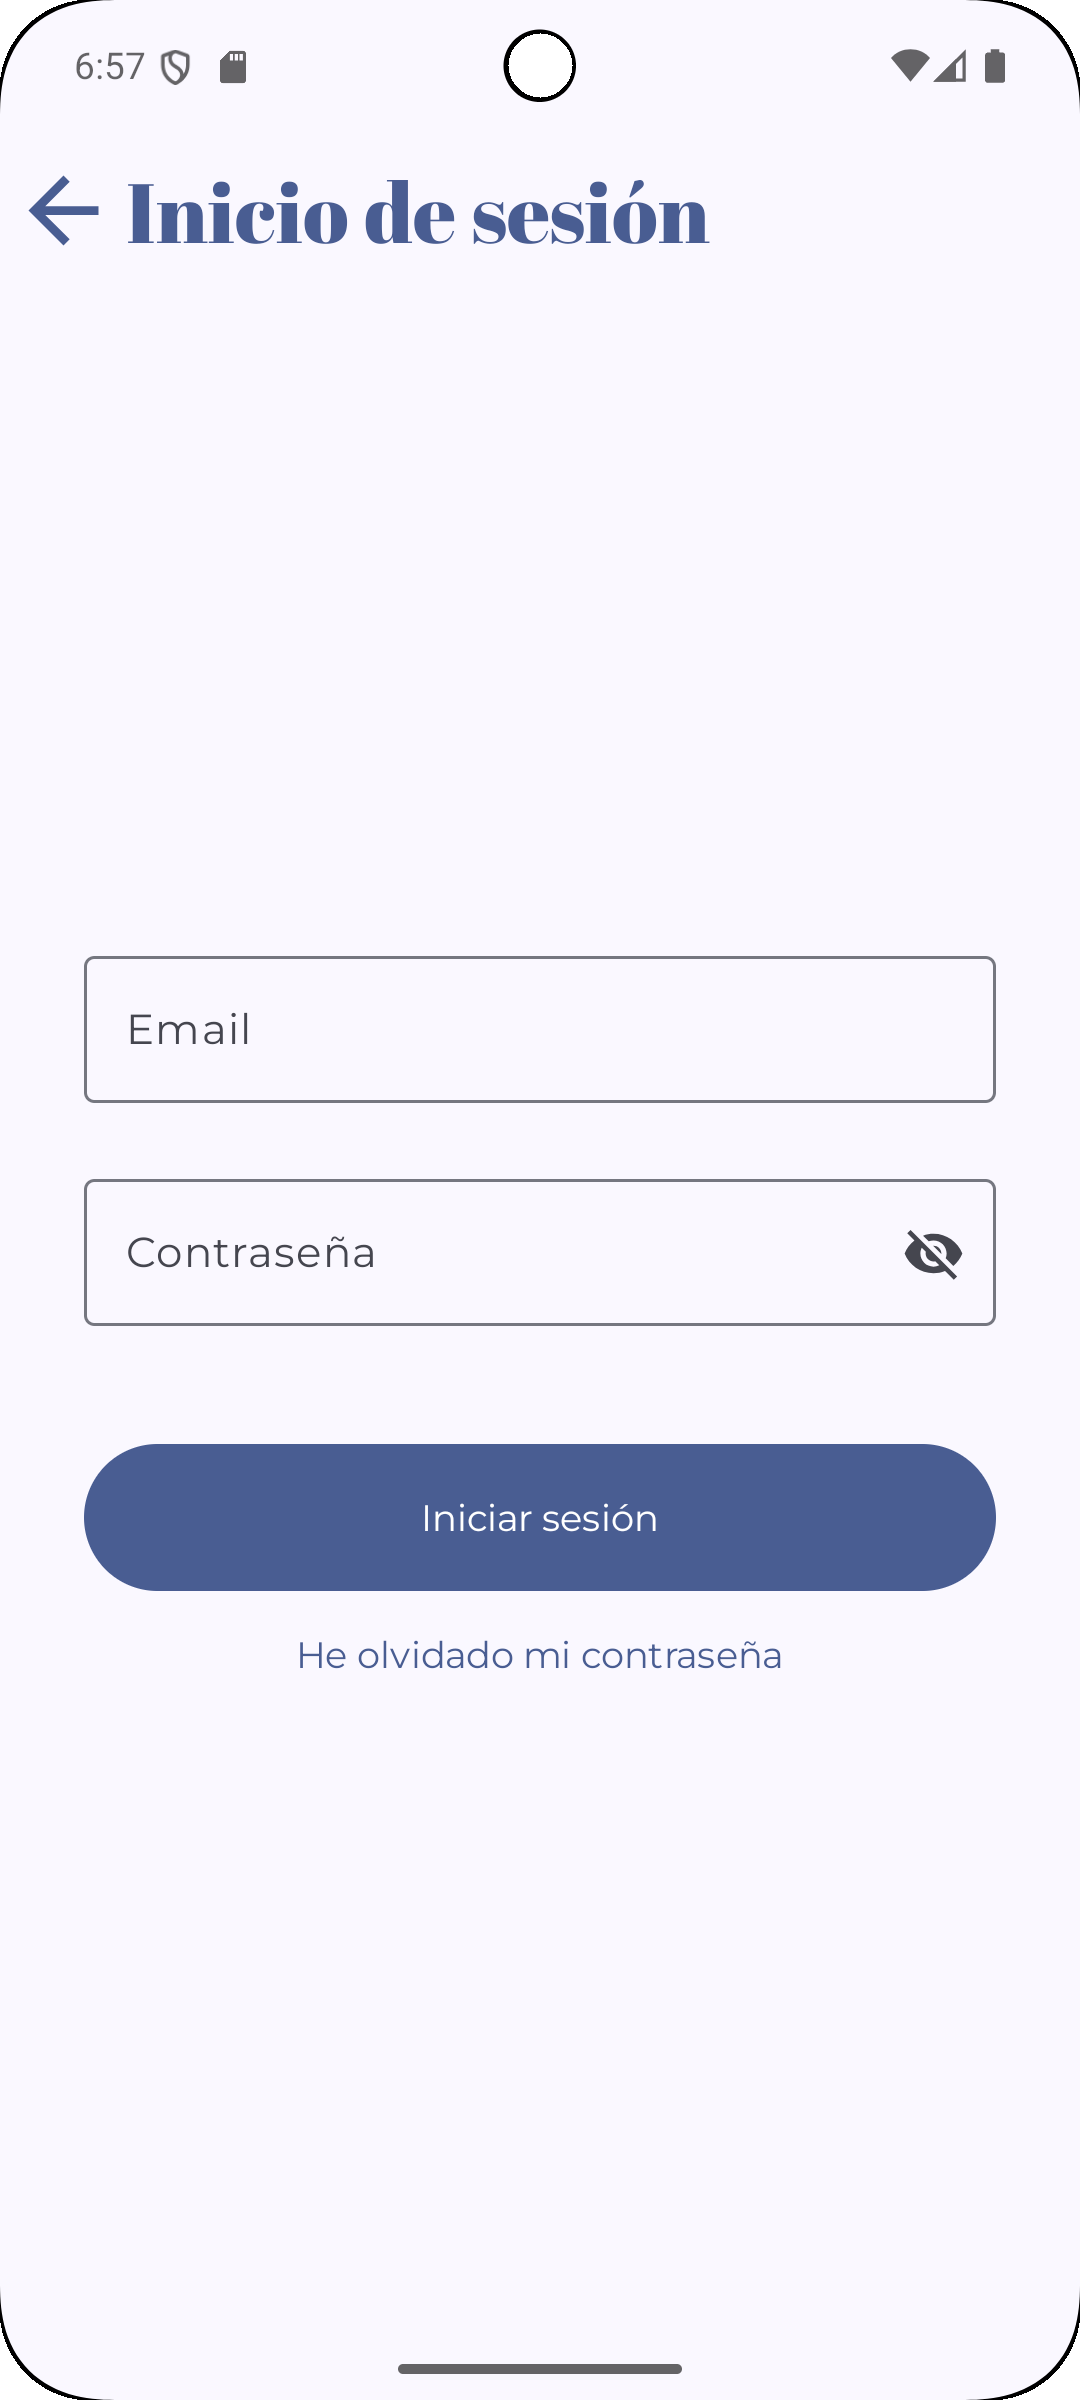
\includegraphics[width=\textwidth]{./img/manual/pinche_login.png}
      \caption{Pantalla de inicio de sesión de un usuario}
      \label{fig:login-main}
    \end{subfigure}
    \hfill
    \begin{subfigure}[b]{0.3\textwidth}
      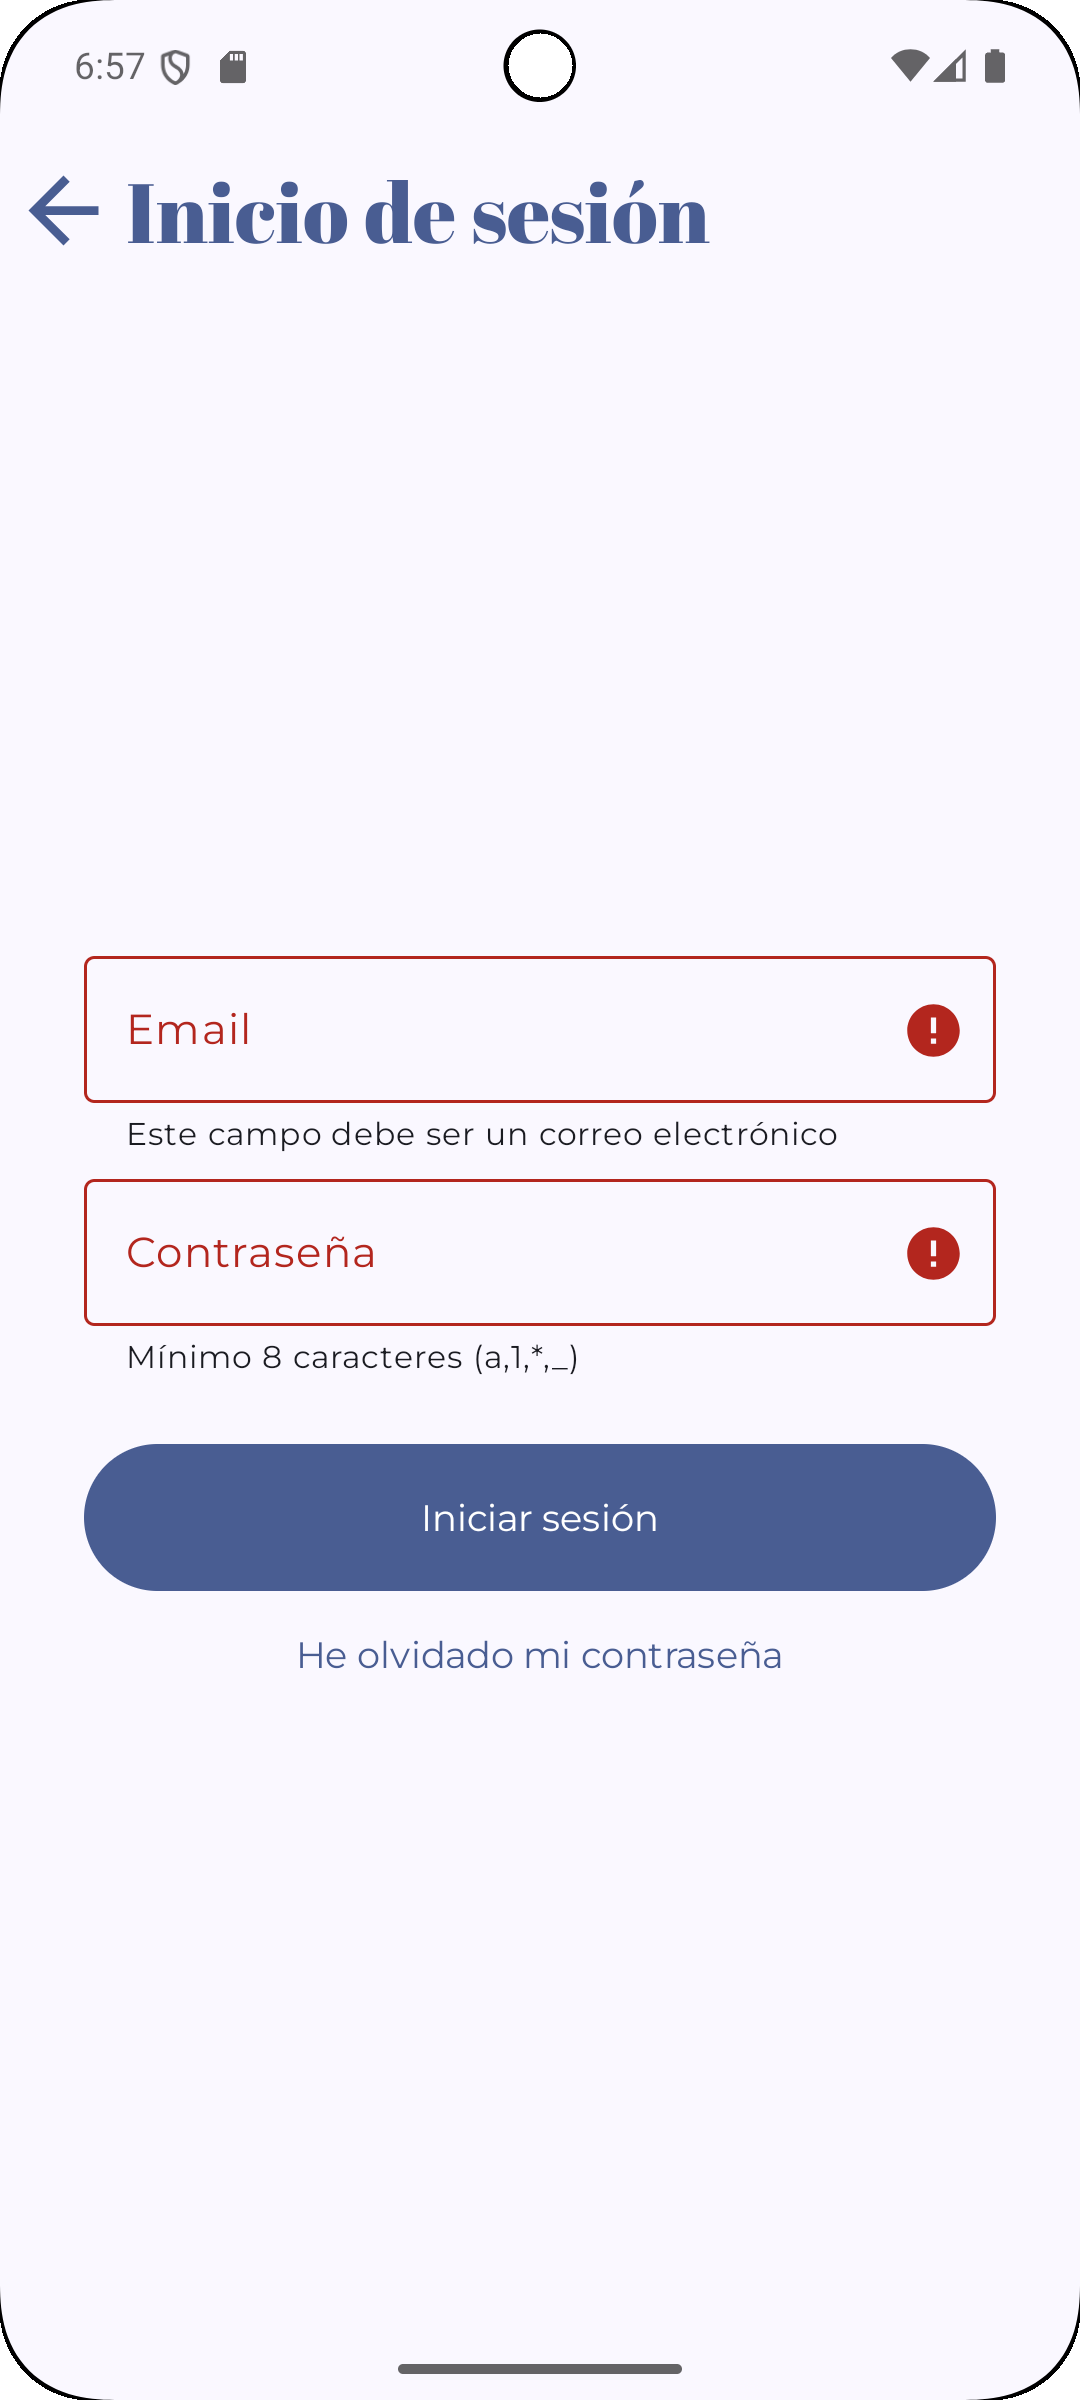
\includegraphics[width=\textwidth]{./img/manual/login_empty_fields.png}
      \caption{Campos obligatorios en la pantalla de inicio de sesión}
      \label{fig:login-must}
    \end{subfigure}
    \hfill
    \begin{subfigure}[b]{0.3\textwidth}
      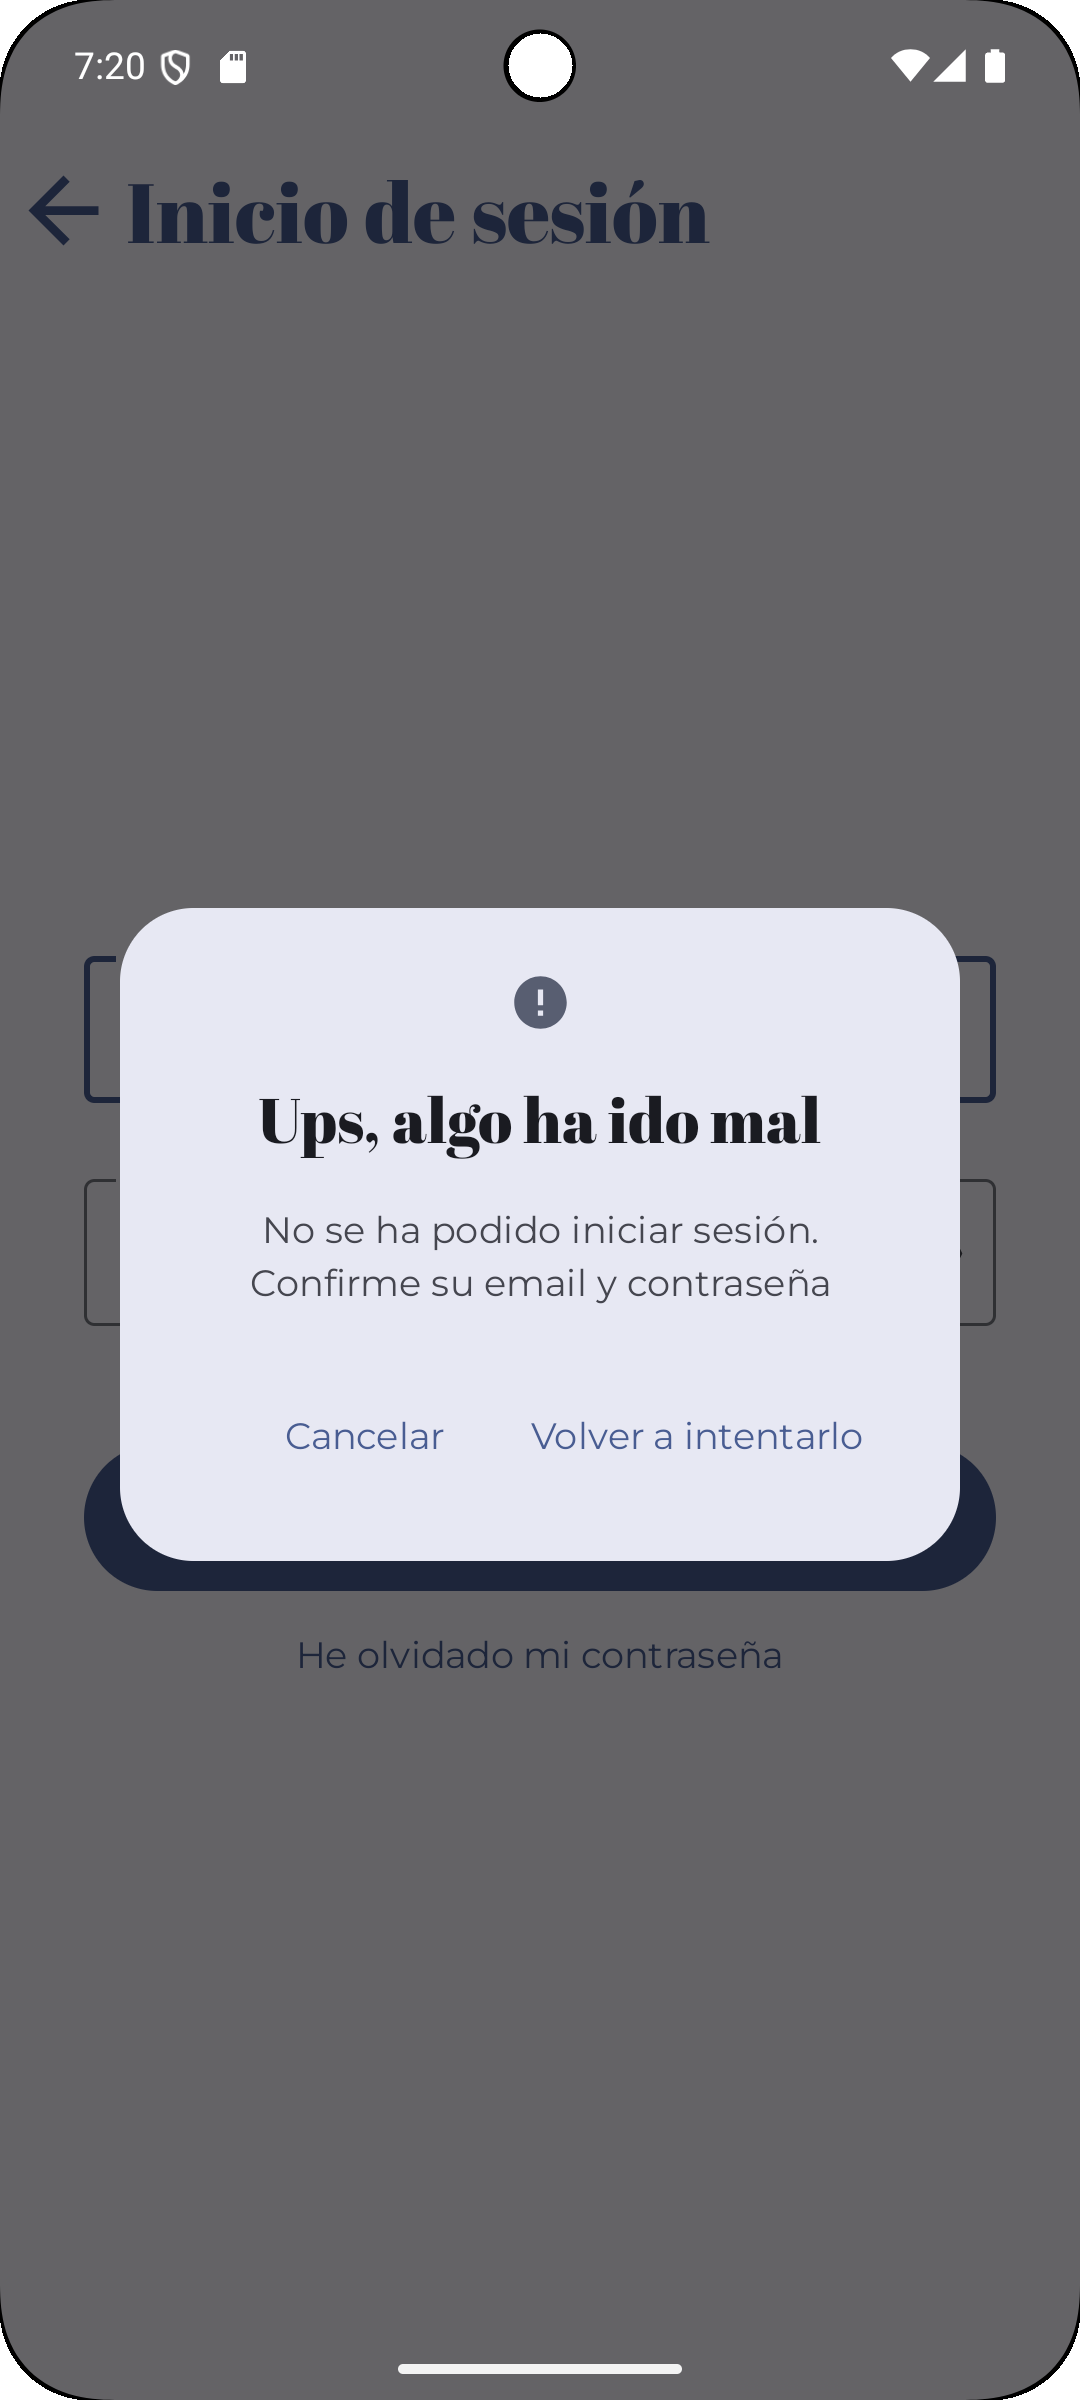
\includegraphics[width=\textwidth]{./img/manual/pinche_login_error.png}
      \caption{Mensaje de error si falla el inicio de sesión de un usuario}
      \label{fig:login-error}
    \end{subfigure}

    \caption{Inicio de sesión}
    \label{fig:login}
\end{figure}

%% reseteo de contraseña
\clearpage
En el caso de que un usuario al iniciar sesión no recuerde su contraseña, accederá a la pantalla de \textbf{recuperar contraseña} en la que introducirá su correo electrónico donde recibirá un enlace para restablecerla Figura~\ref{fig:reset-password-main}. Si el envío del correo electrónico ha sido exitoso se le mostrará un mensaje confirmando el envío Figura~\ref{fig:reset-password-succeeds}.

\begin{figure}[H]
    \centering

    \begin{subfigure}[b]{0.3\textwidth}
      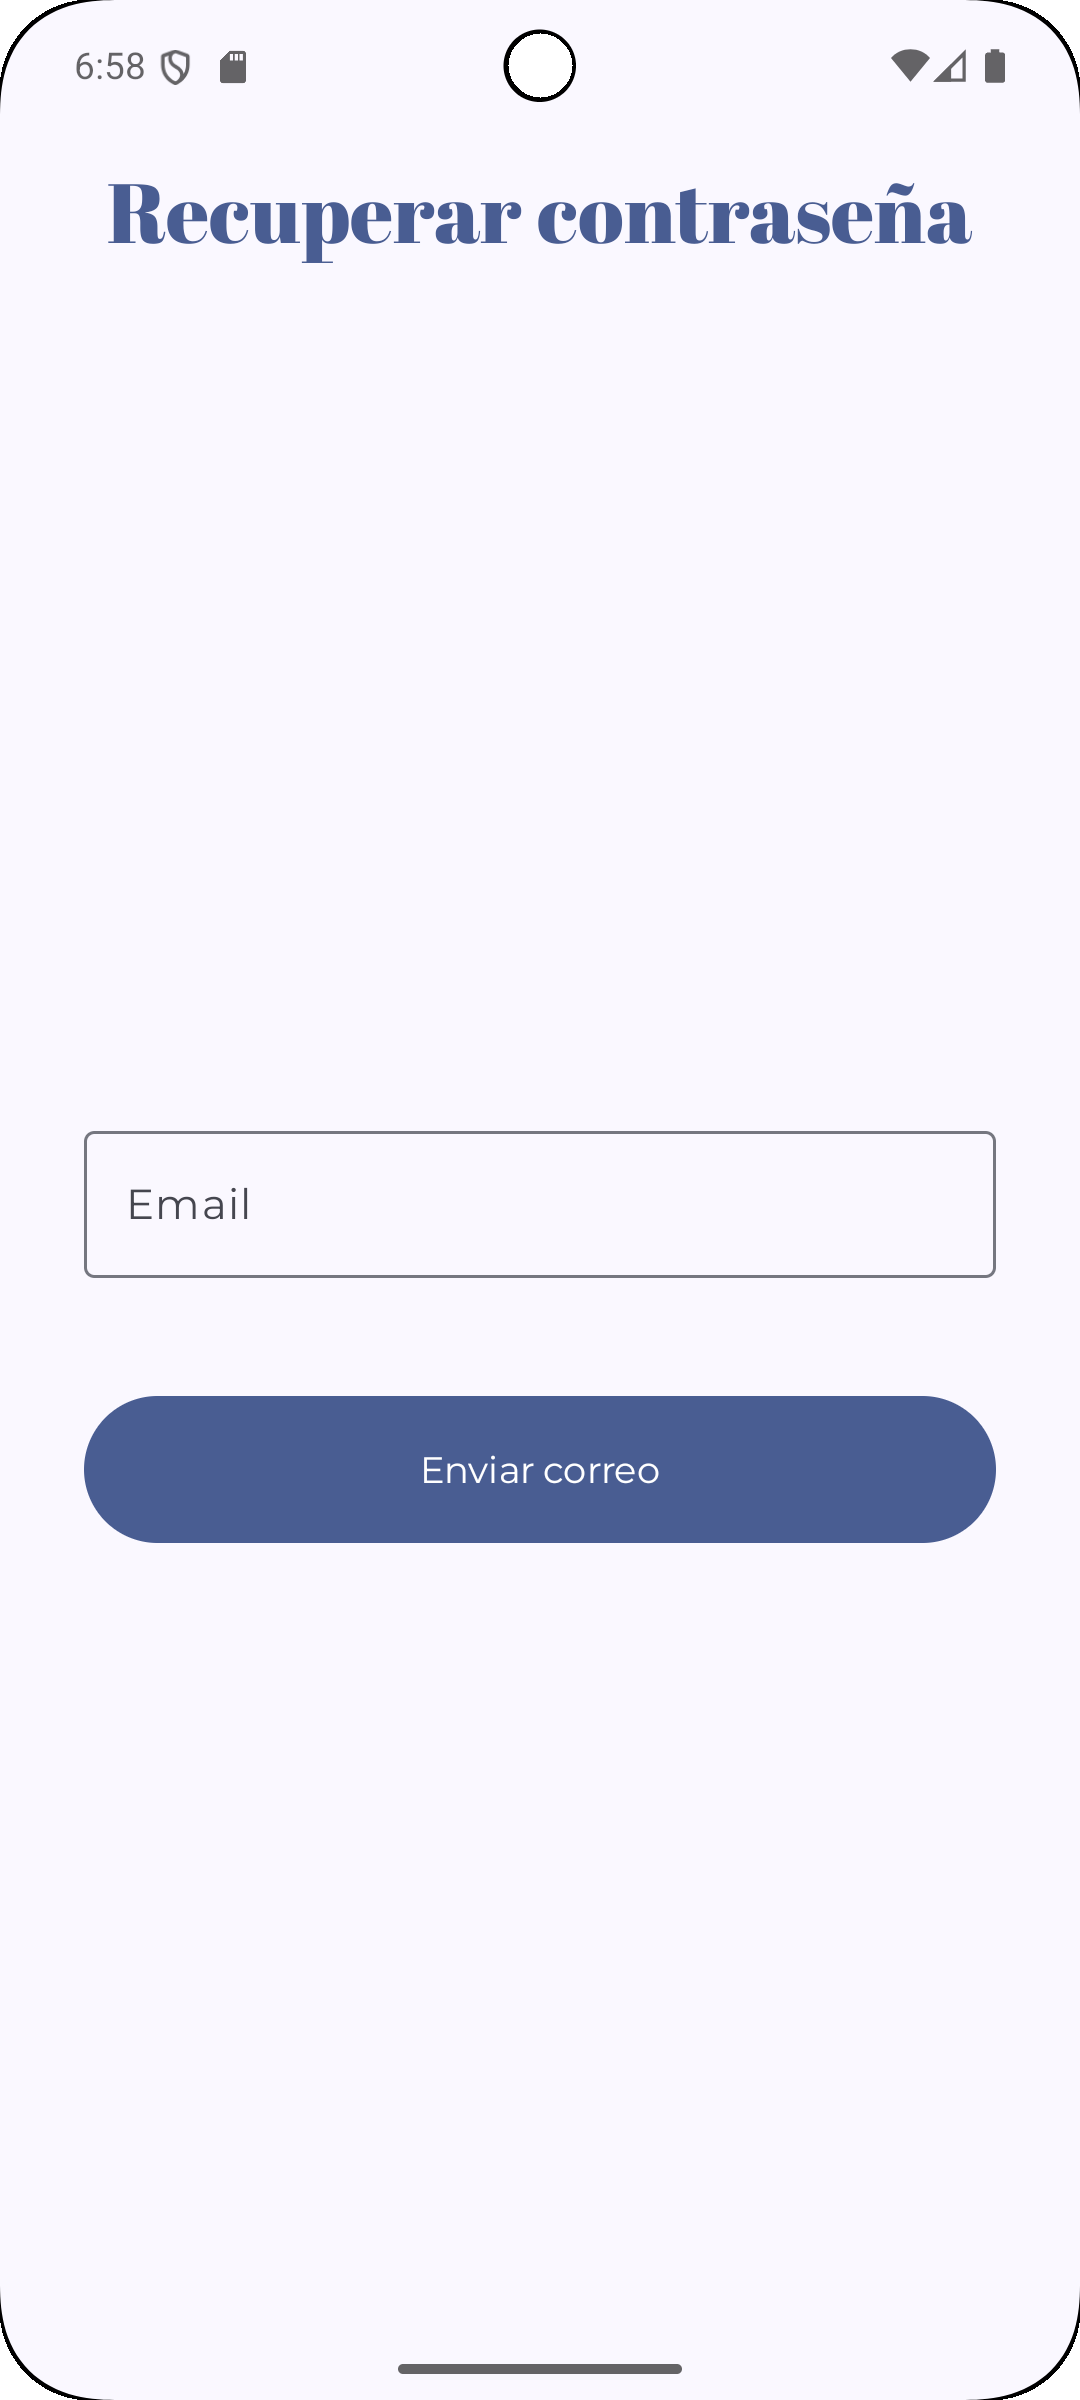
\includegraphics[width=\textwidth]{./img/manual/sent_reset_password_email.png}
      \caption{Pantalla de recuperar contraseña}
      \label{fig:reset-password-main}
    \end{subfigure}
    \hfill
    \begin{subfigure}[b]{0.3\textwidth}
      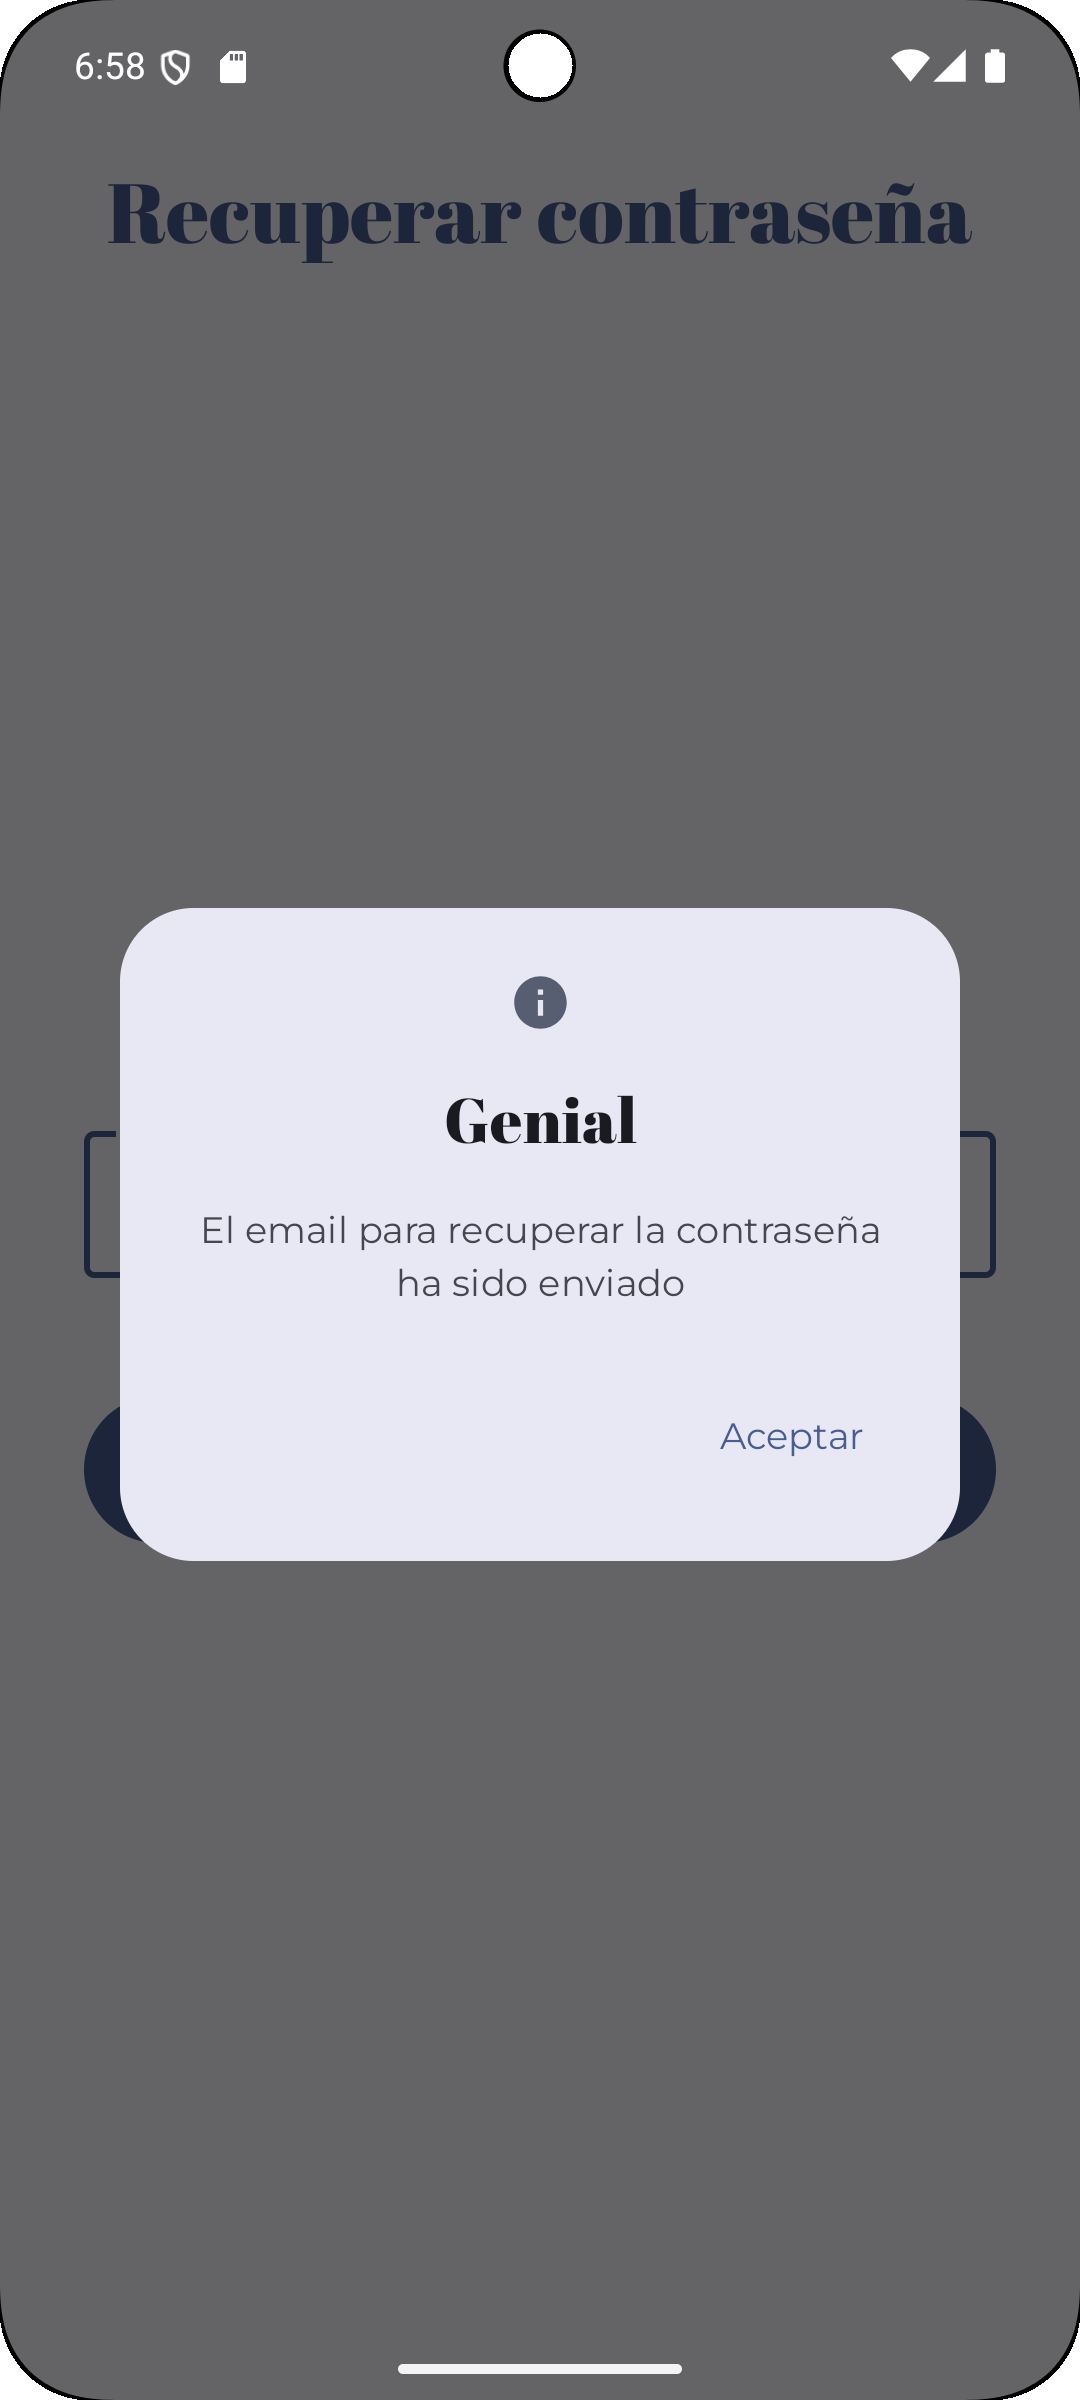
\includegraphics[width=\textwidth]{./img/manual/send_email_success.png}
      \caption{Envío exitoso del correo electrónico}
      \label{fig:reset-password-succeeds}
    \end{subfigure}
    \hfill
    \caption{Aviso de envío de correo electrónico para recuperar contraseña}
    \label{fig:reset-password}
\end{figure}

%% home
\clearpage
Si el registro o el login se han efectuado con éxito, el usuario aparece en la pantalla \textbf{principal} Figura~\ref{fig:main}.

\begin{figure}[H]
\centering
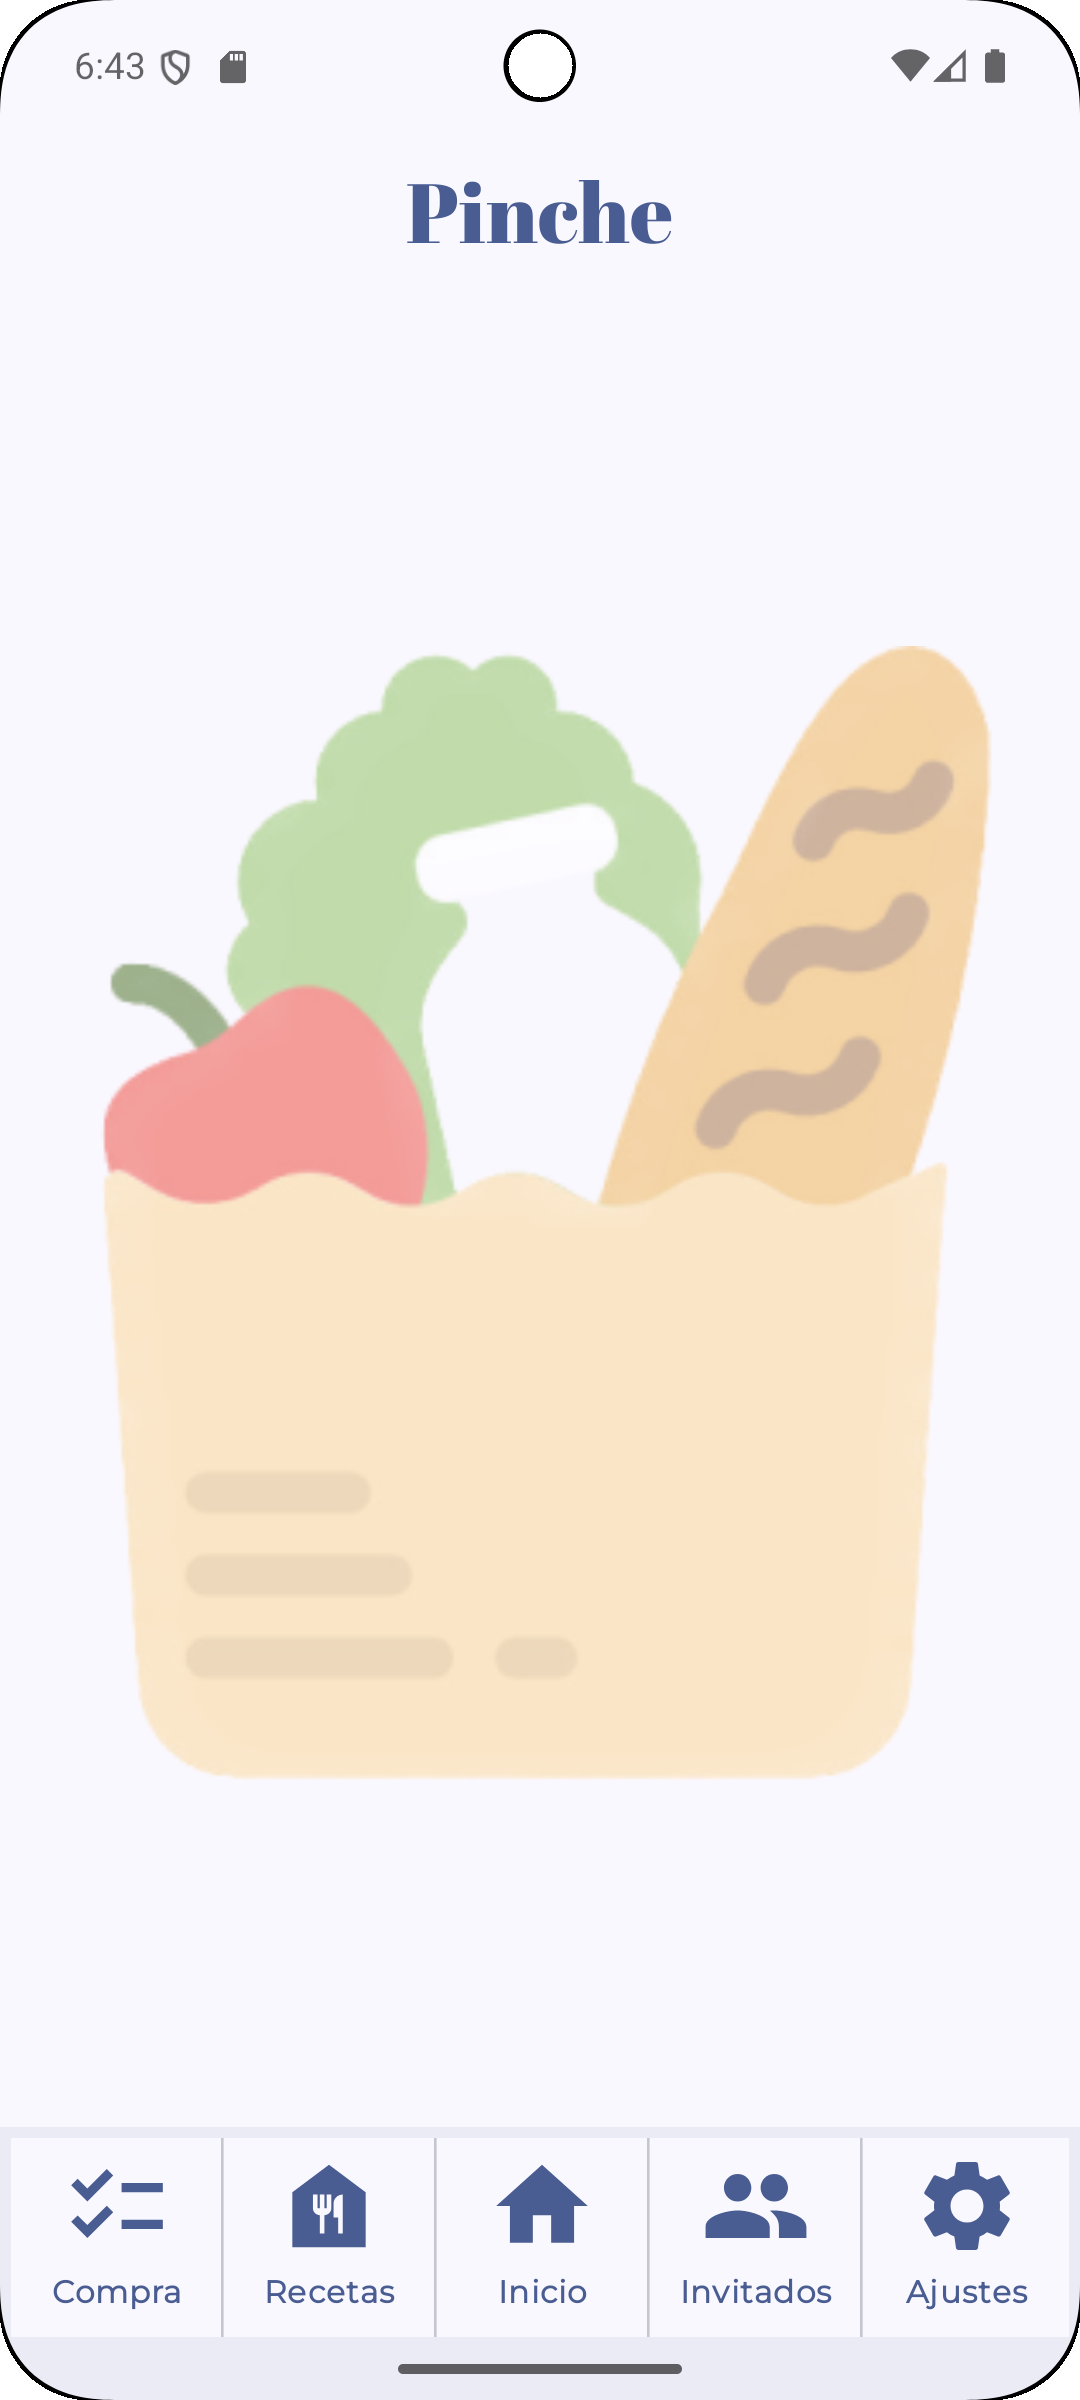
\includegraphics[width=0.3\textwidth]{./img/manual/pinche_home.png}
\caption{Pantalla principal de Pinche}
\label{fig:main}
\end{figure}

%% gestión cuenta de usuario
\clearpage
Desde la pantalla principal puede acceder a los \textbf{ajustes}. Donde podrá ver estadísticas sobre su uso en la aplicación y gestionar su cuenta Figura~\ref{fig:settings-main}. Desde esta pantalla puede cerrar sesión, confirmando la acción con un aviso de lo que supone realizarla Figura~\ref{fig:sign-out}. También puede eliminar su cuenta, confirmando la acción tras un aviso con las consecuencias de esta acción Figura~\ref{fig:delete}.

\begin{figure}[H]
    \centering

    \begin{subfigure}[b]{0.3\textwidth}
      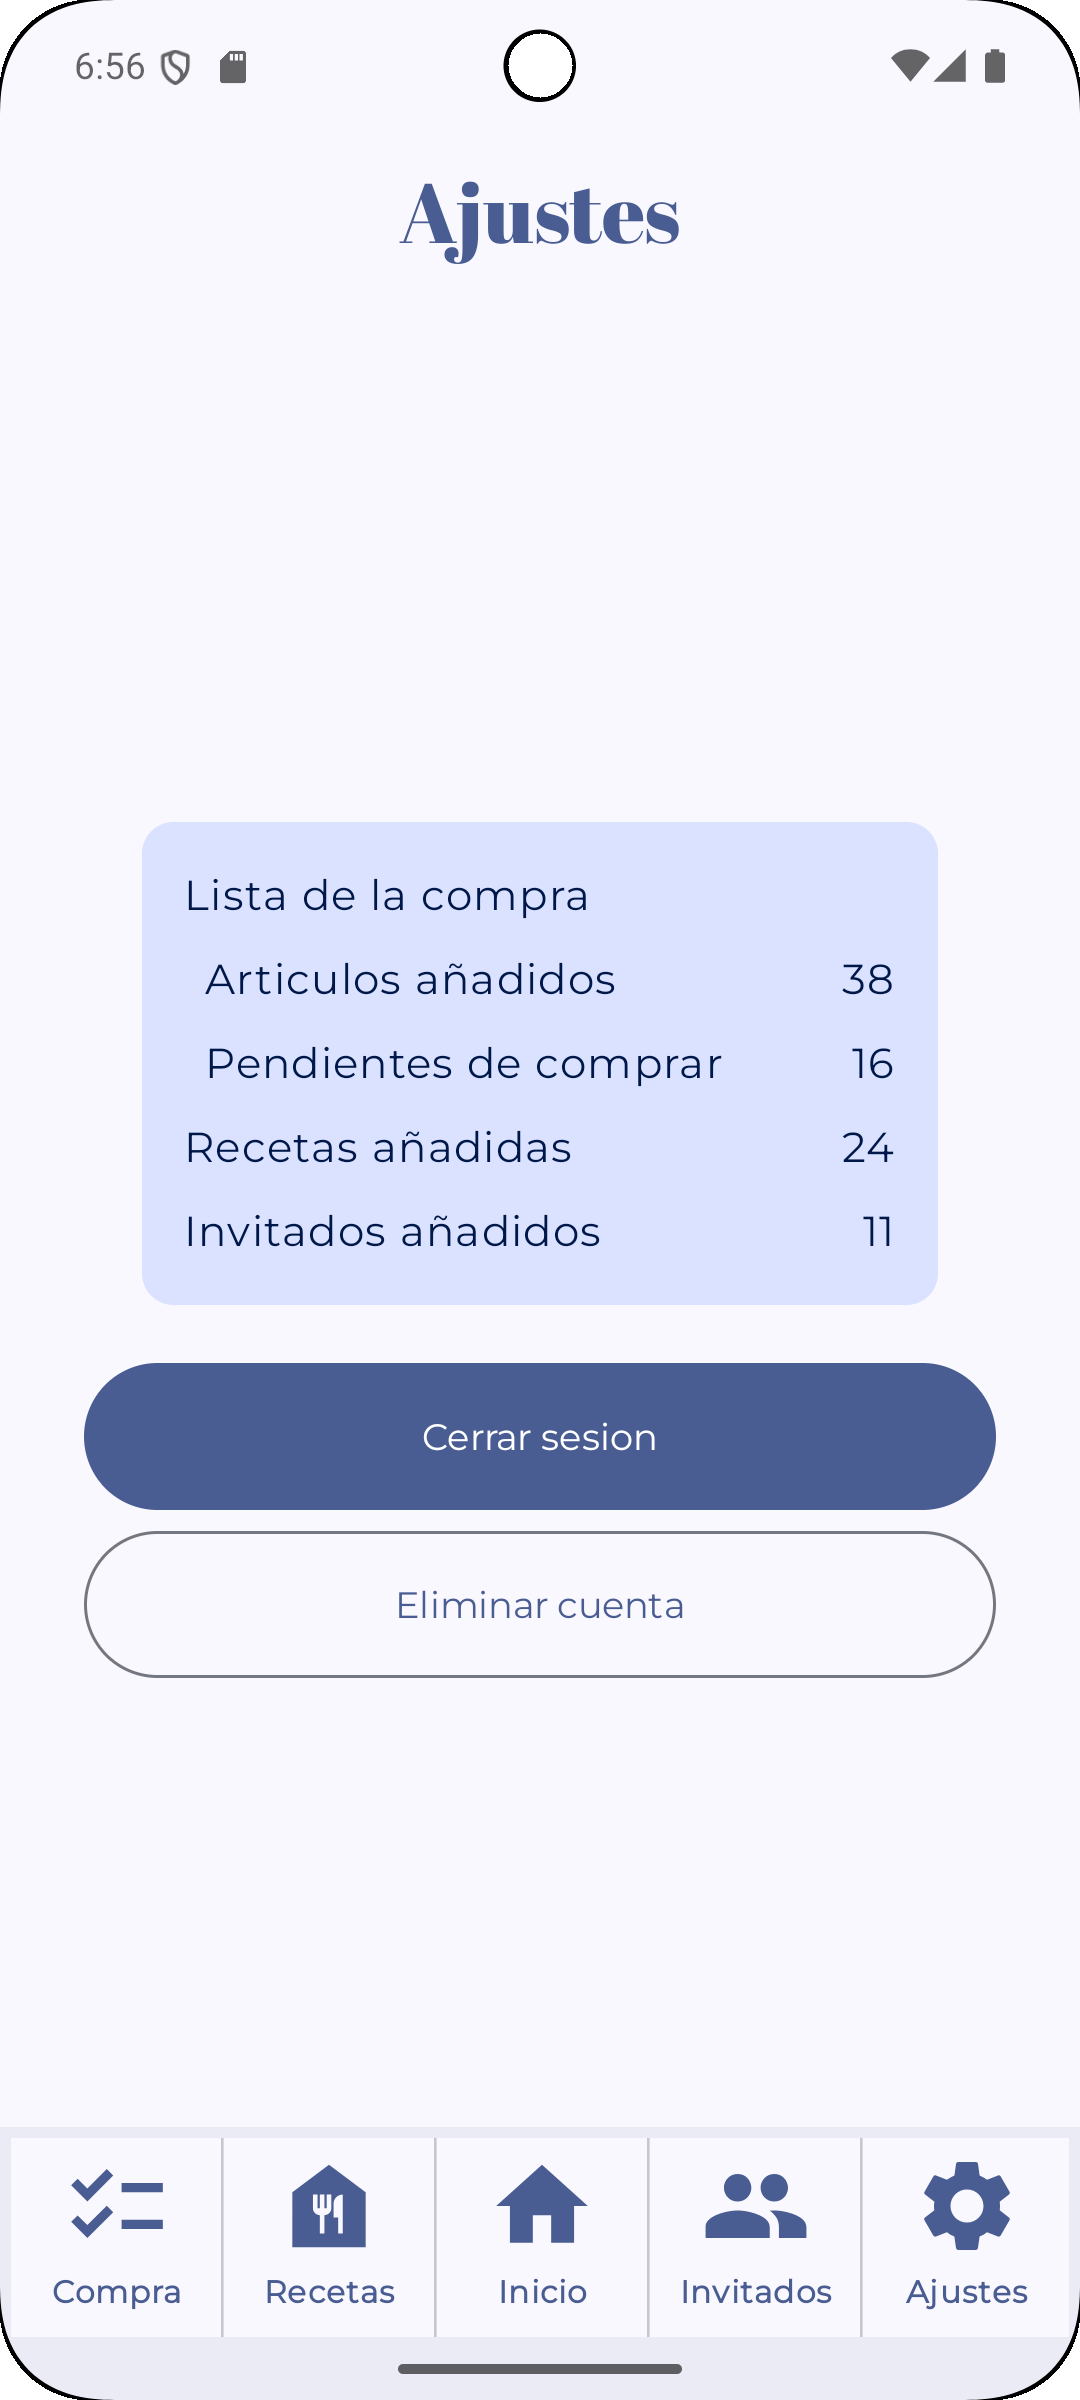
\includegraphics[width=\textwidth]{./img/manual/pinche_settings.png}
      \caption{Pantalla de ajustes}
      \label{fig:settings-main}
    \end{subfigure}
    \hfill
    \begin{subfigure}[b]{0.3\textwidth}
      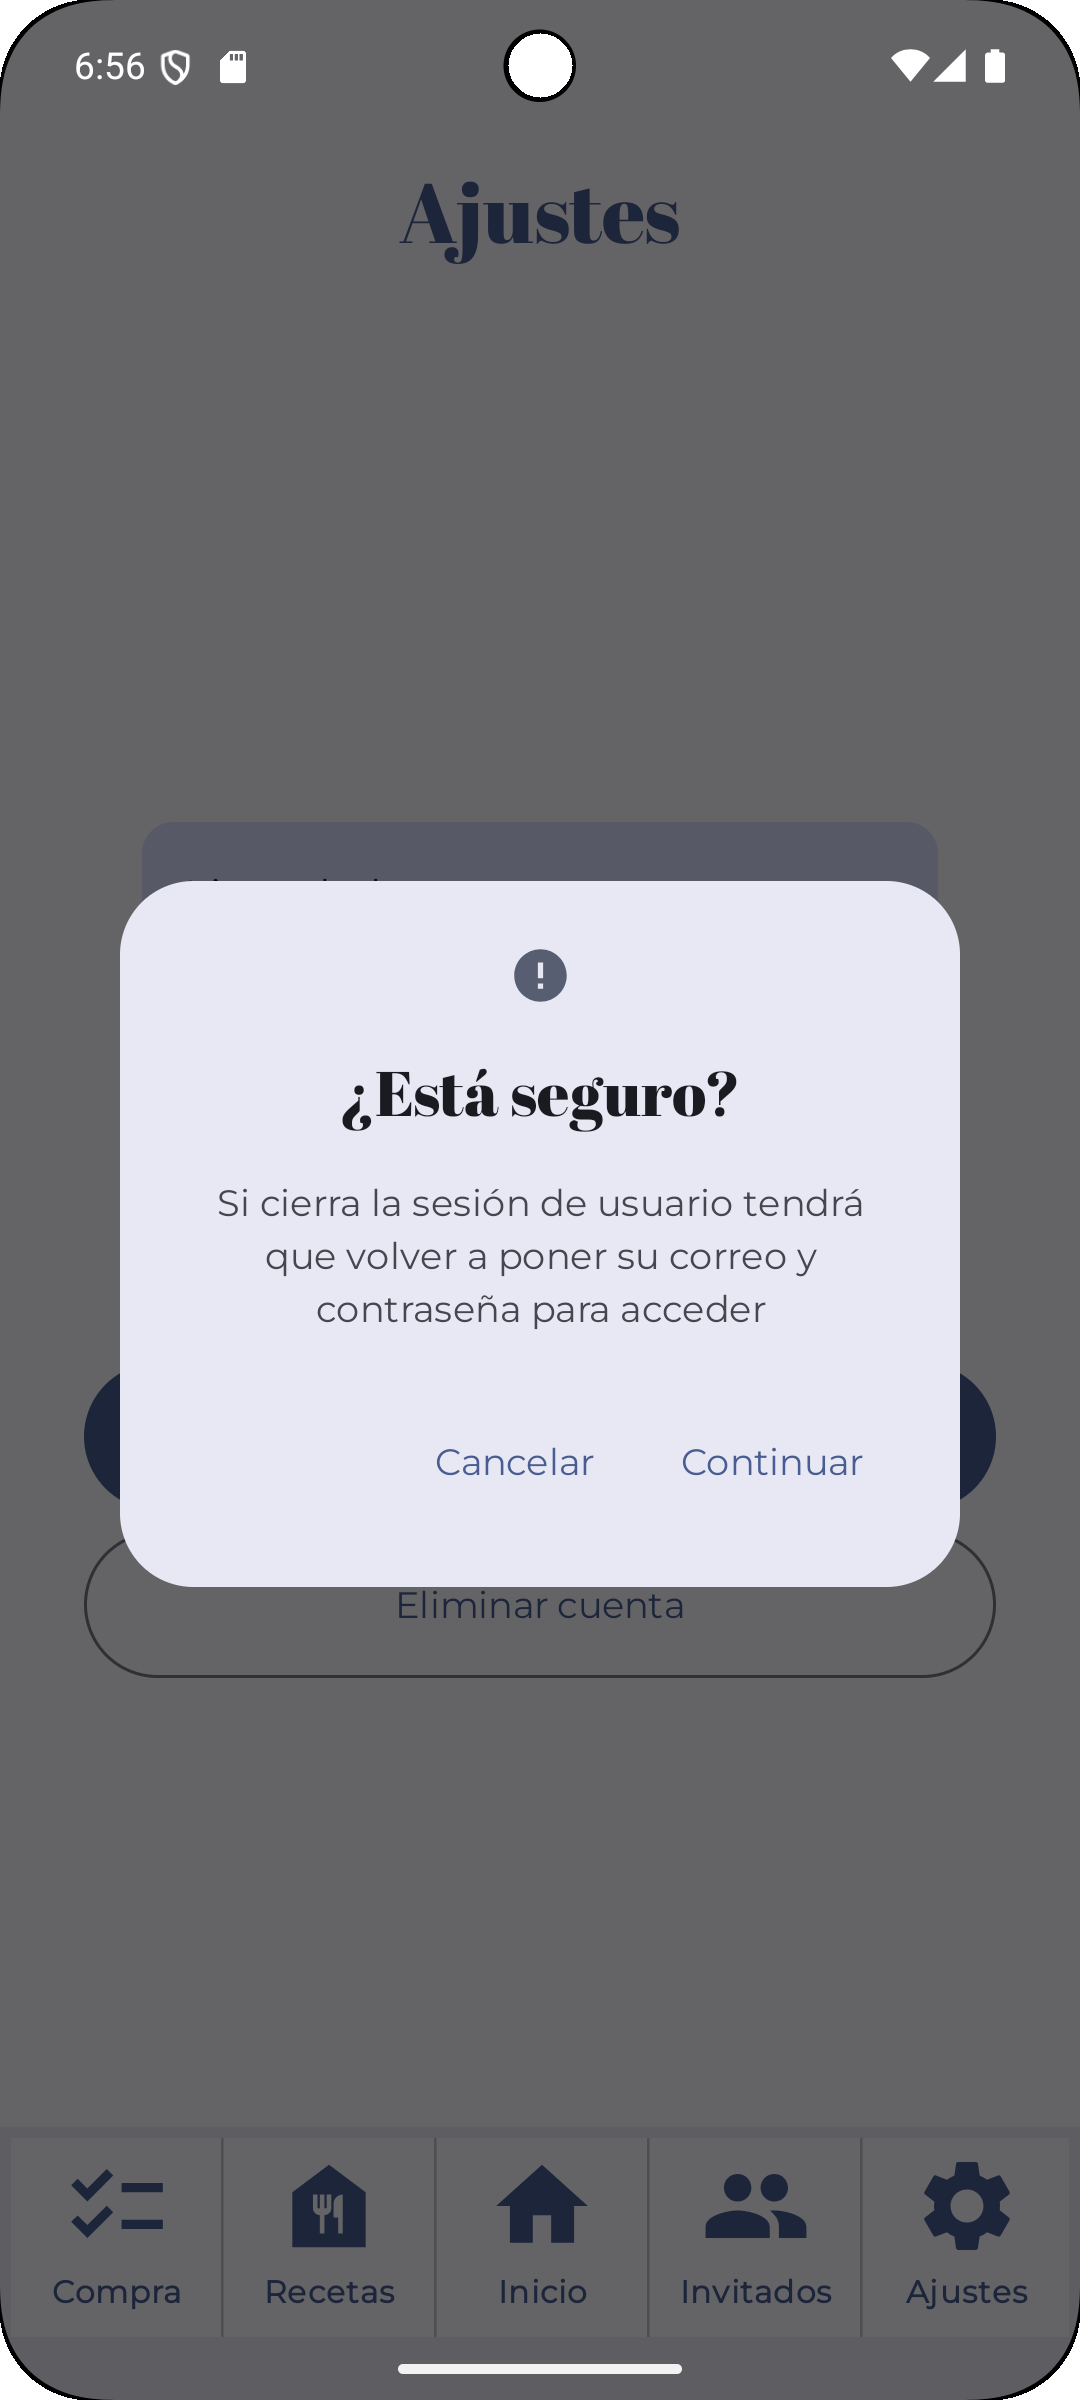
\includegraphics[width=\textwidth]{./img/manual/sign_out_confirm.png}
      \caption{Cerrar sesión}
      \label{fig:sign-out}
    \end{subfigure}
    \hfill
    \begin{subfigure}[b]{0.3\textwidth}
      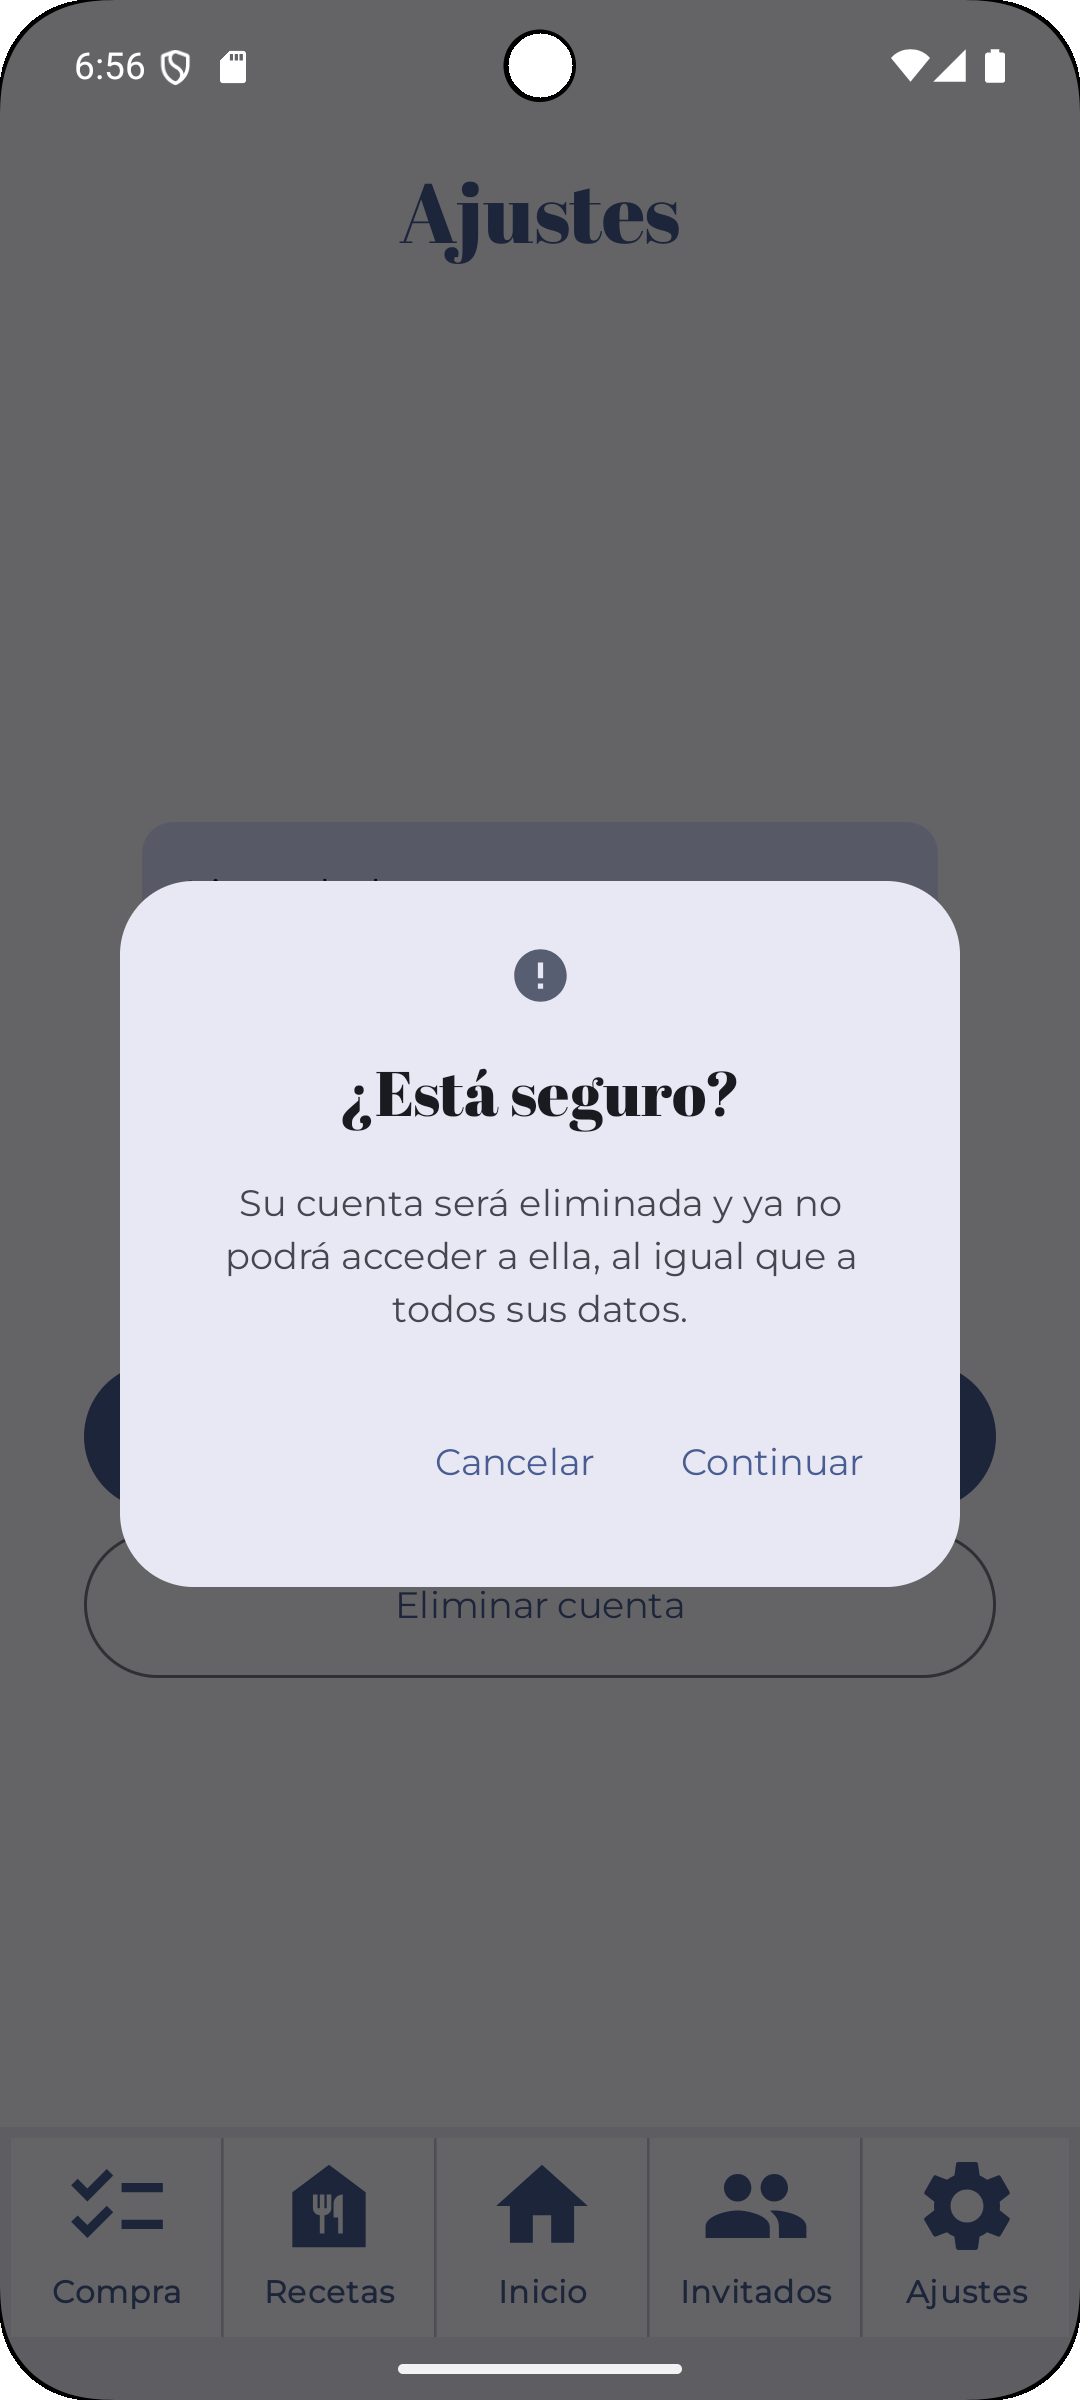
\includegraphics[width=\textwidth]{./img/manual/delete_account_confirm.png}
      \caption{Eliminar cuenta}
      \label{fig:delete}
    \end{subfigure}

    \caption{Ajustes}
    \label{fig:settings}
\end{figure}

%% lista de la compra
Desde la pantalla principal también puede acceder a la sección de \textbf{listas de la compra}. Si no hay listas de la compra, se mostrará el estado de la pantalla de listas de la compra vacía Figura~\ref{fig:shopping}. En el caso de que sí tenga listas de la compra se le muestran al usuario Figura~\ref{fig:shopping-empty}. Desde aquí podrá añadir una lista de la compra, acceder al detalle de las listas que ya tenga, ver qué listas tienen todos sus artículos comprados y cuáles tiene artículos pendientes Figura~\ref{fig:complete-or-not-shopping} y eliminar una lista tras confirmar la acción Figura~\ref{fig:delete-shopping}.

\begin{figure}[H]
    \centering

    \begin{subfigure}[b]{0.3\textwidth}
      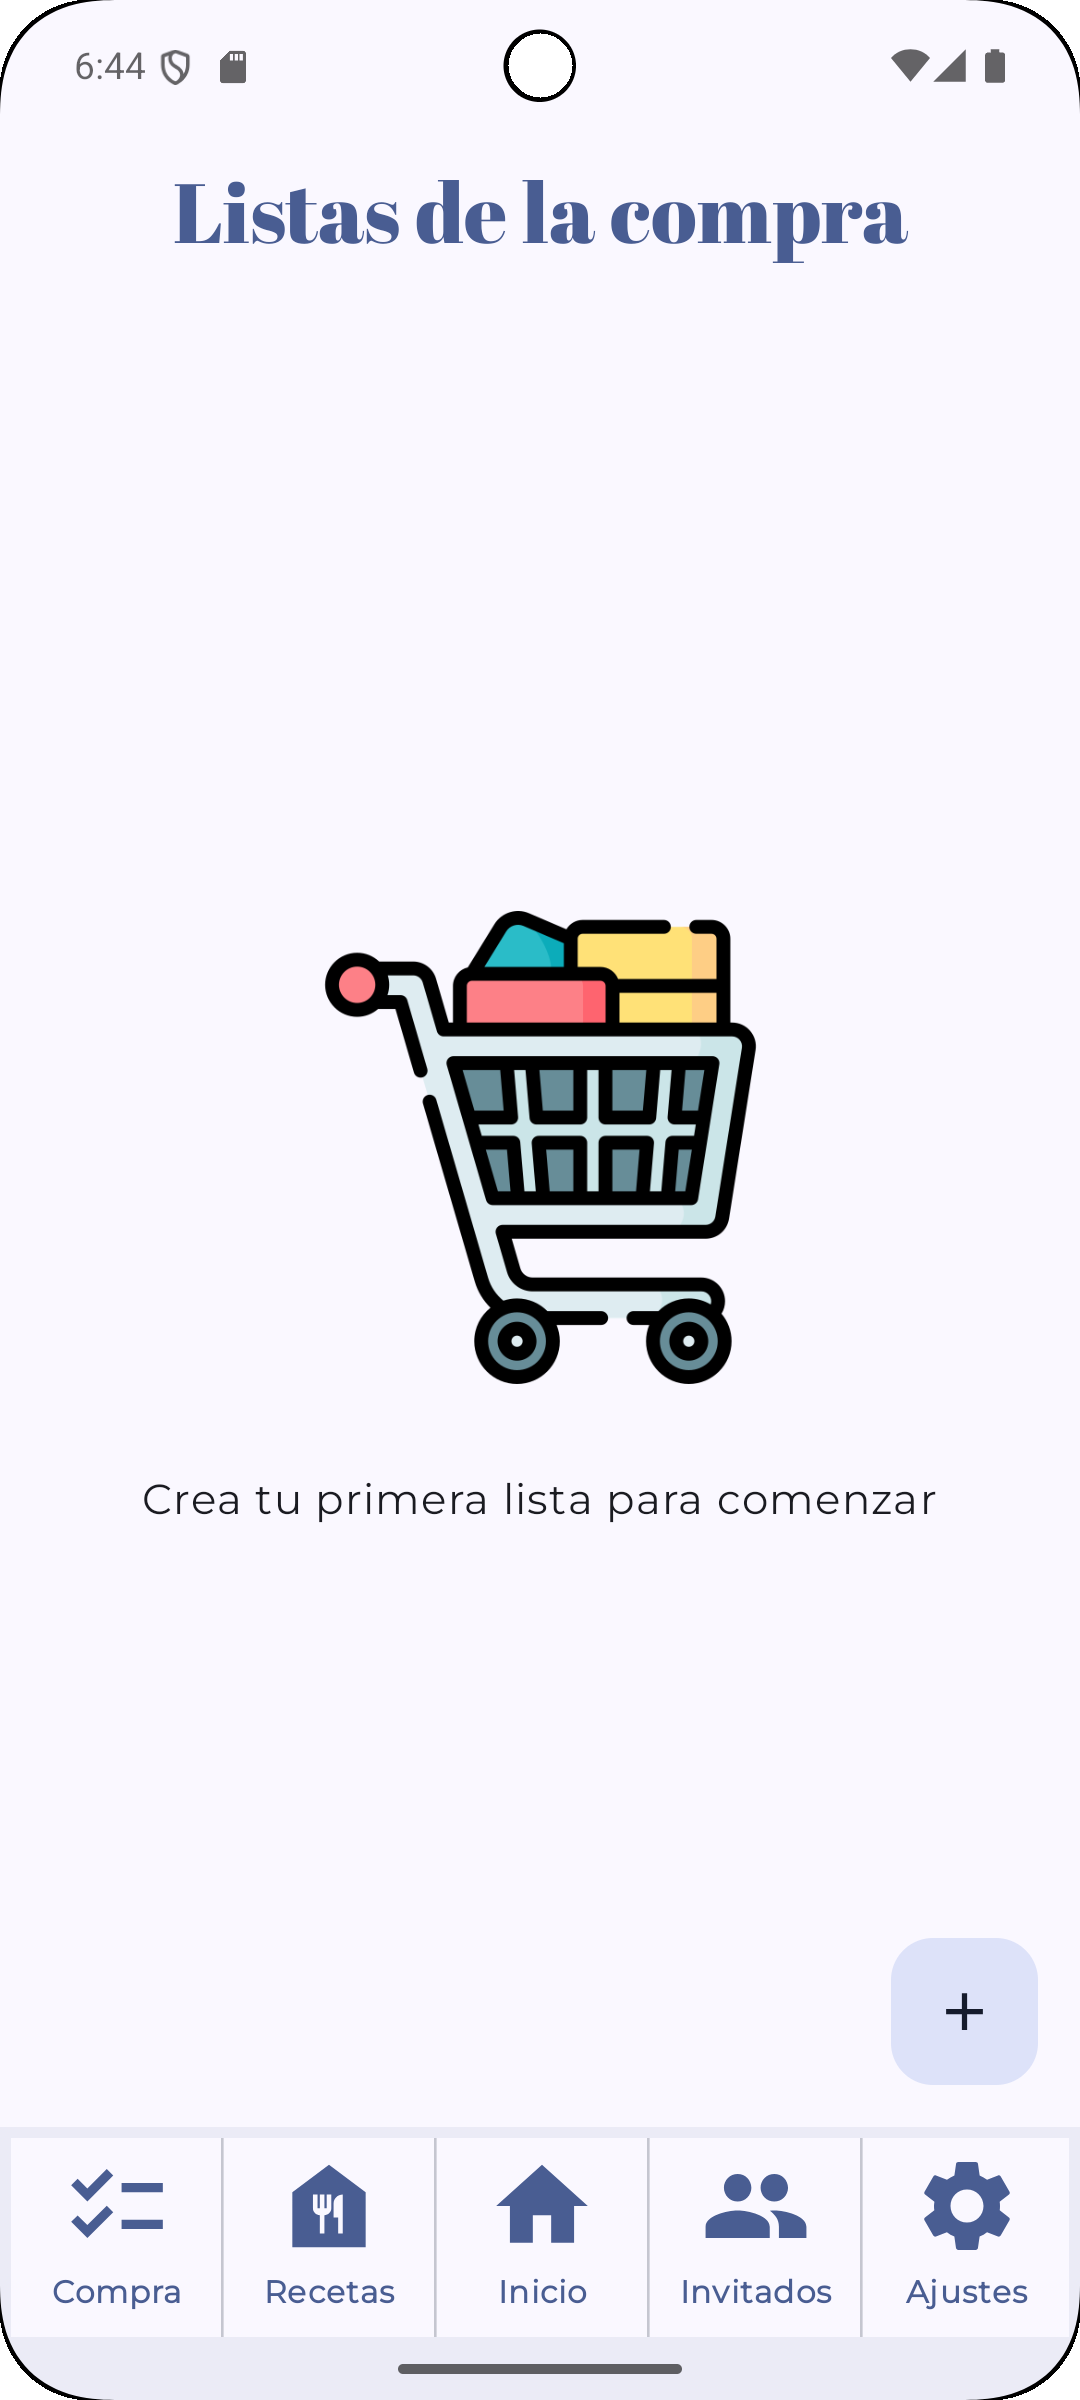
\includegraphics[width=\textwidth]{./img/manual/pinche_empty_shopping_list.png}
      \caption{Pantalla vacía de listas de la compra}
      \label{fig:shopping-empty}
    \end{subfigure}
    \hfill
    \begin{subfigure}[b]{0.3\textwidth}
      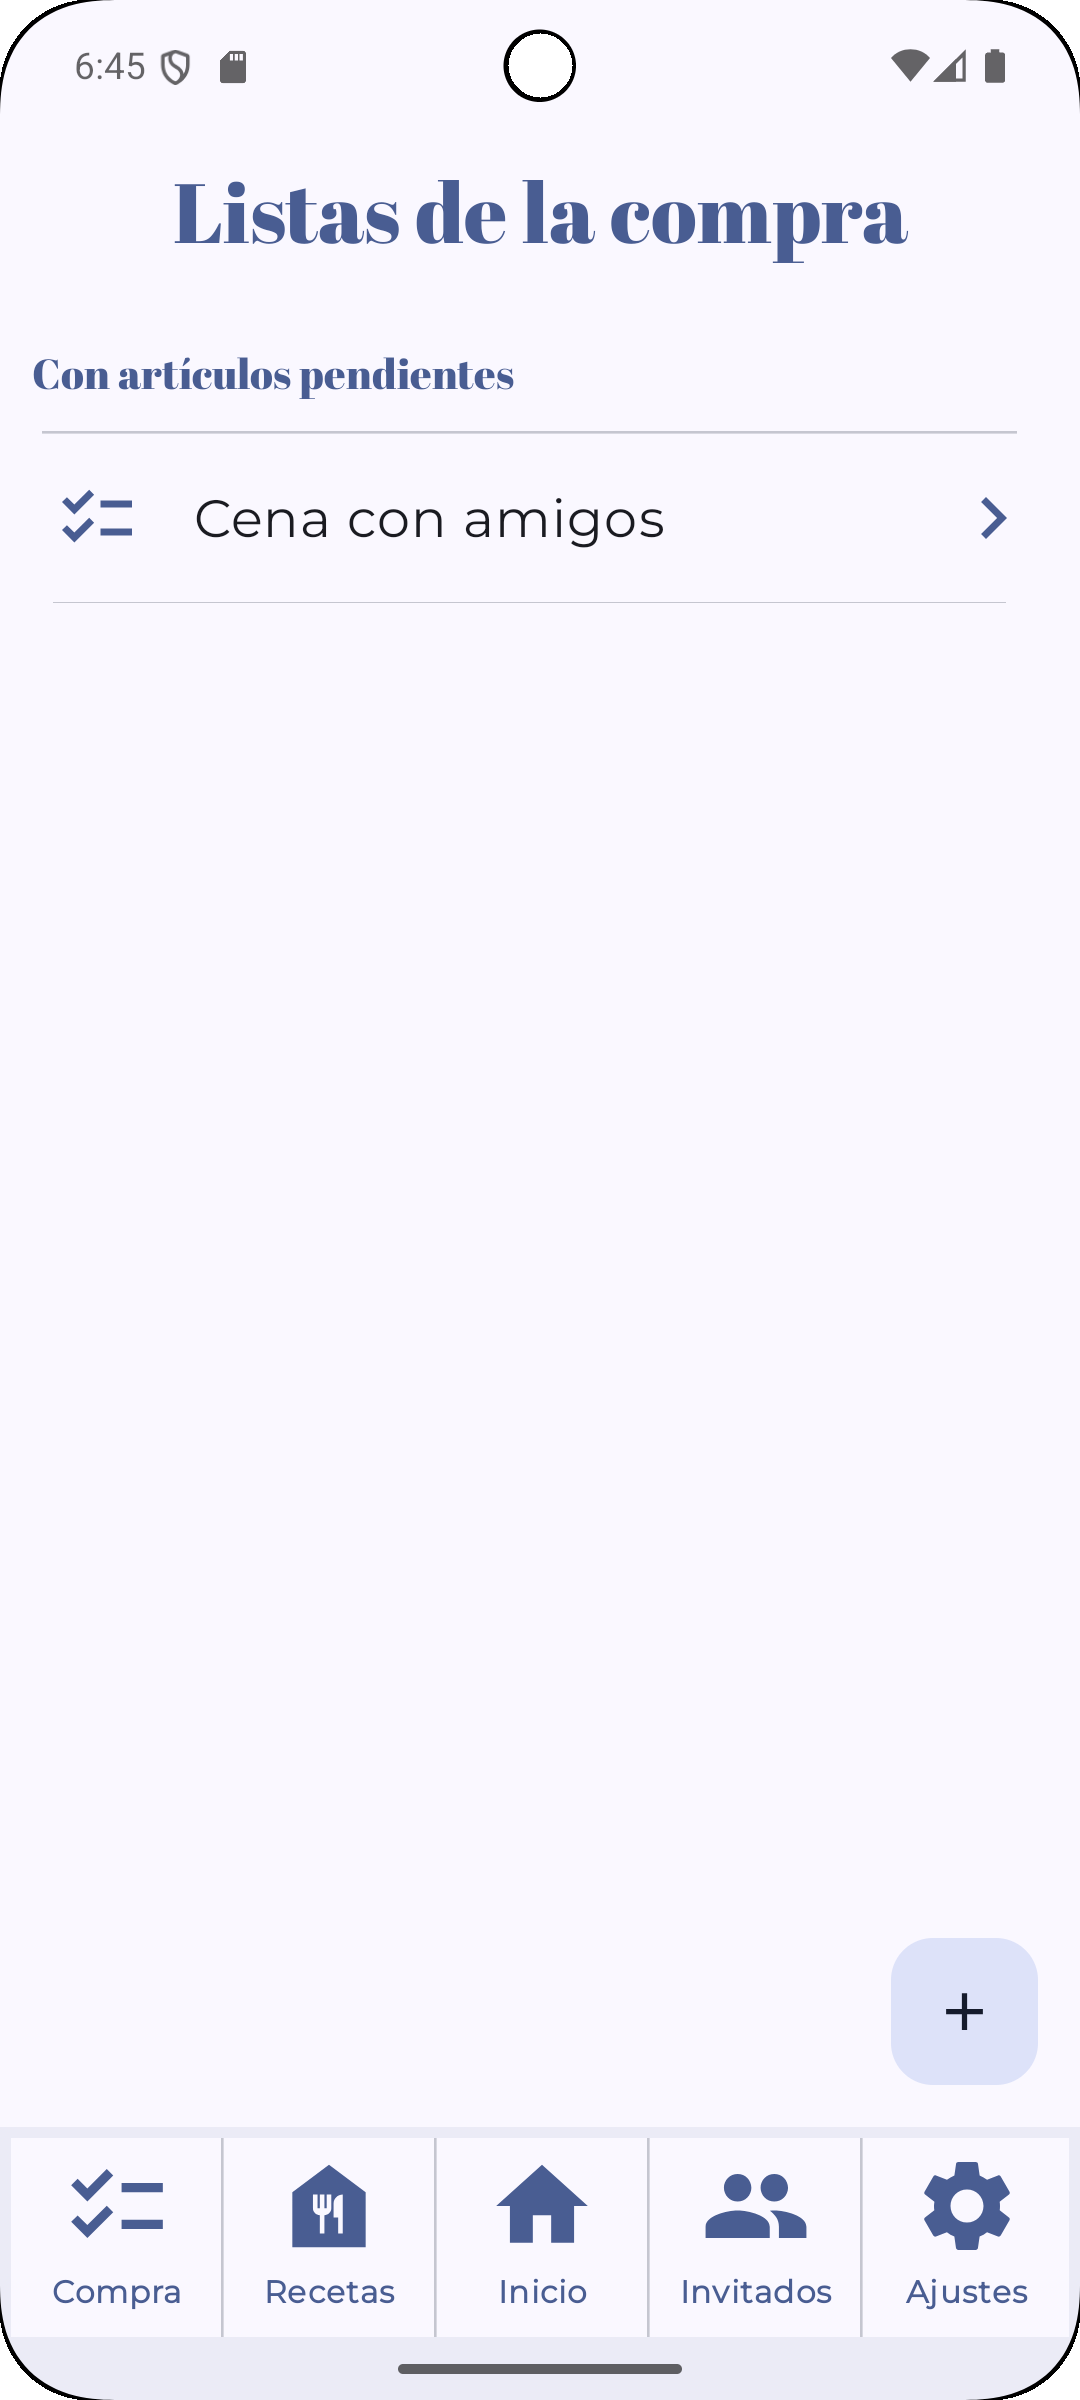
\includegraphics[width=\textwidth]{./img/manual/pinche_one_shopping_list.png}
      \caption{Pantalla de listas de la compra}
      \label{fig:shopping}
    \end{subfigure}

    \begin{subfigure}[b]{0.3\textwidth}
      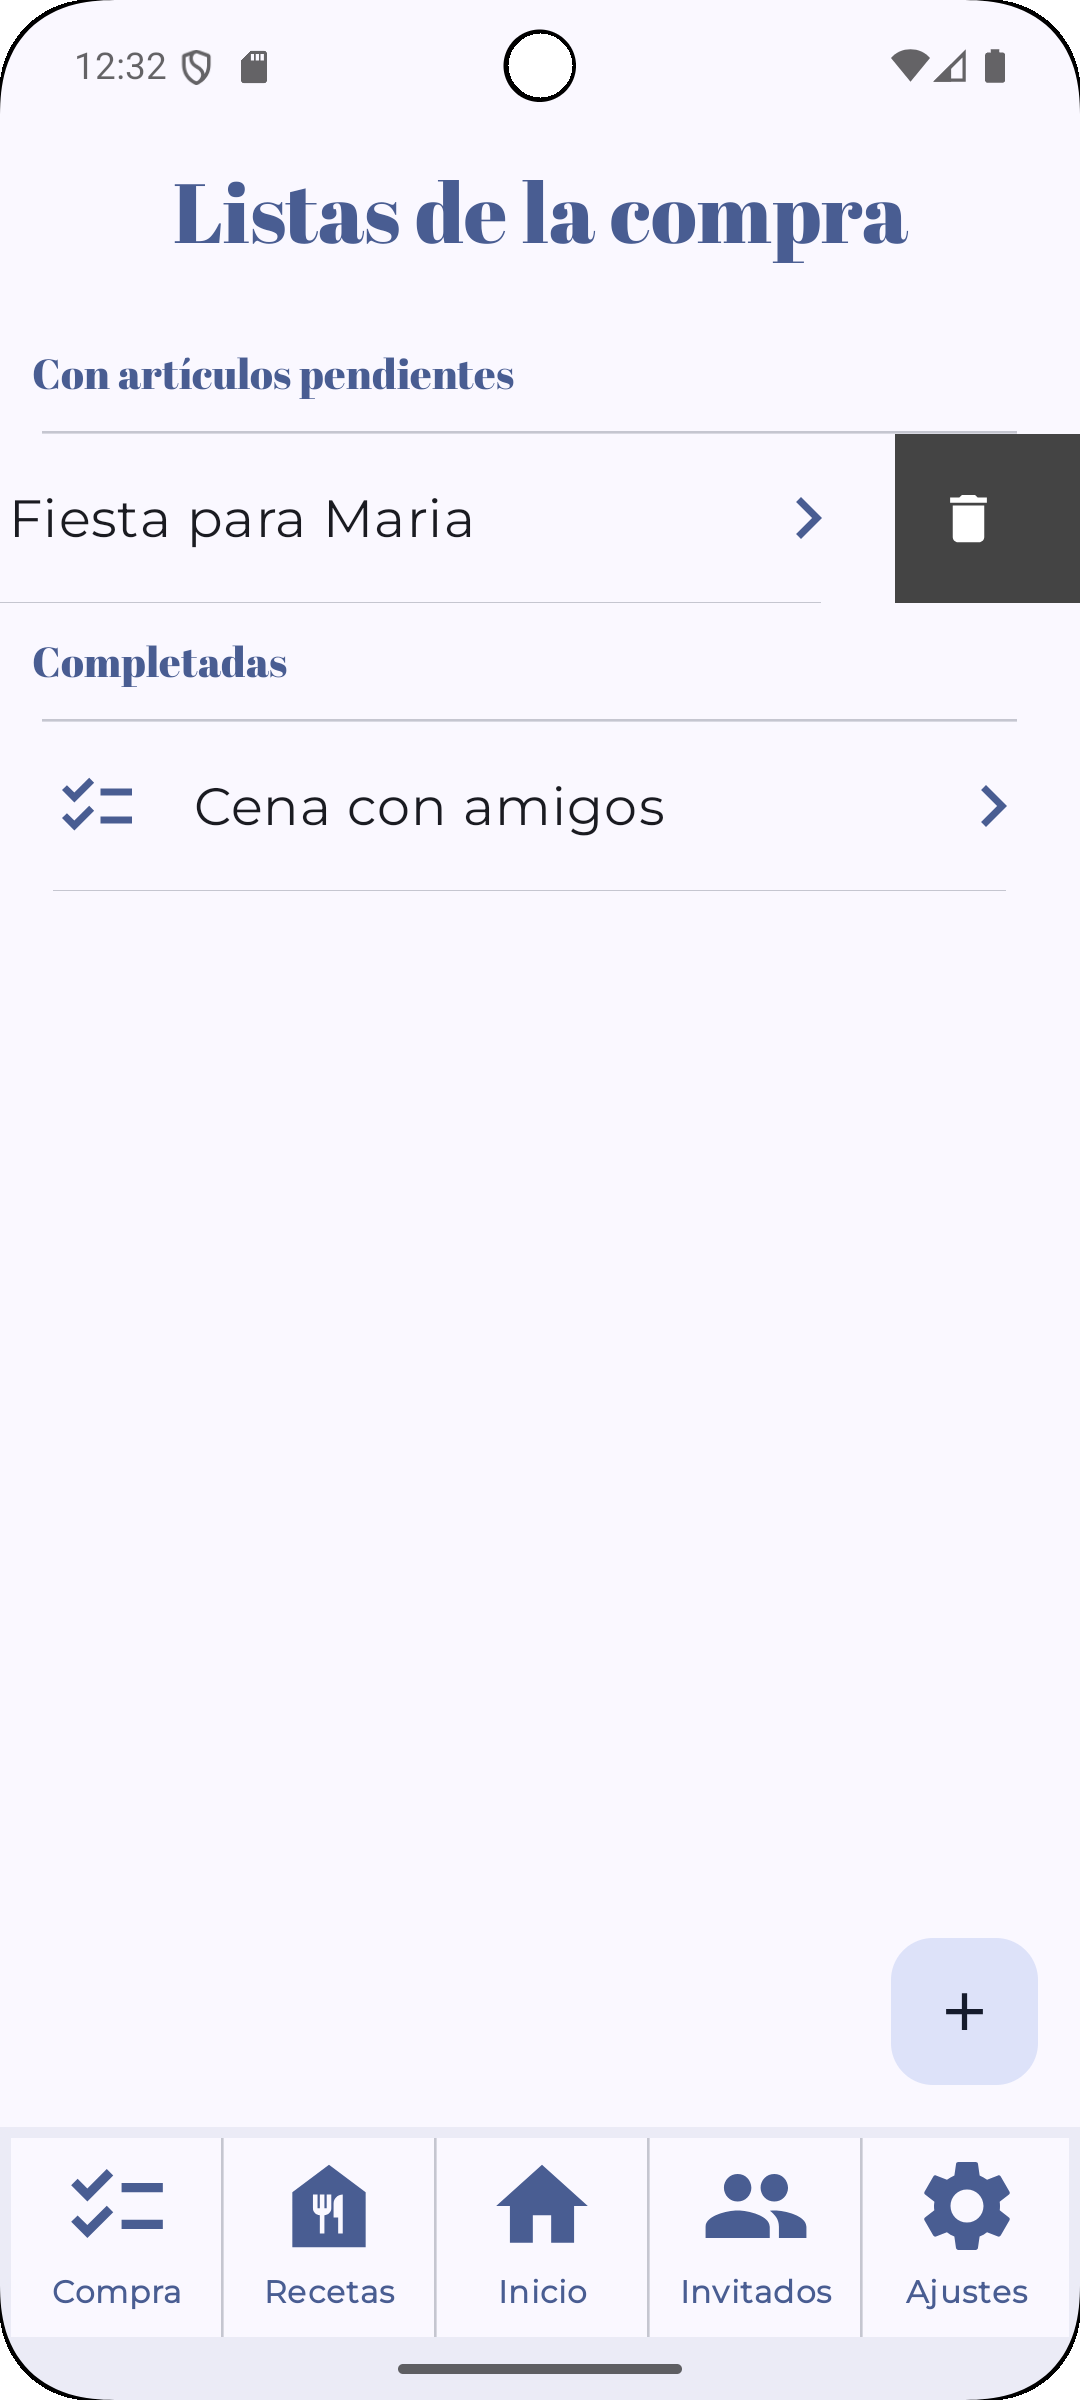
\includegraphics[width=\textwidth]{./img/manual/delete_shopping.png}
      \caption{Eliminar lista de la compra}
      \label{fig:delete-shopping}
    \end{subfigure}
    \hfill
    \begin{subfigure}[b]{0.3\textwidth}
      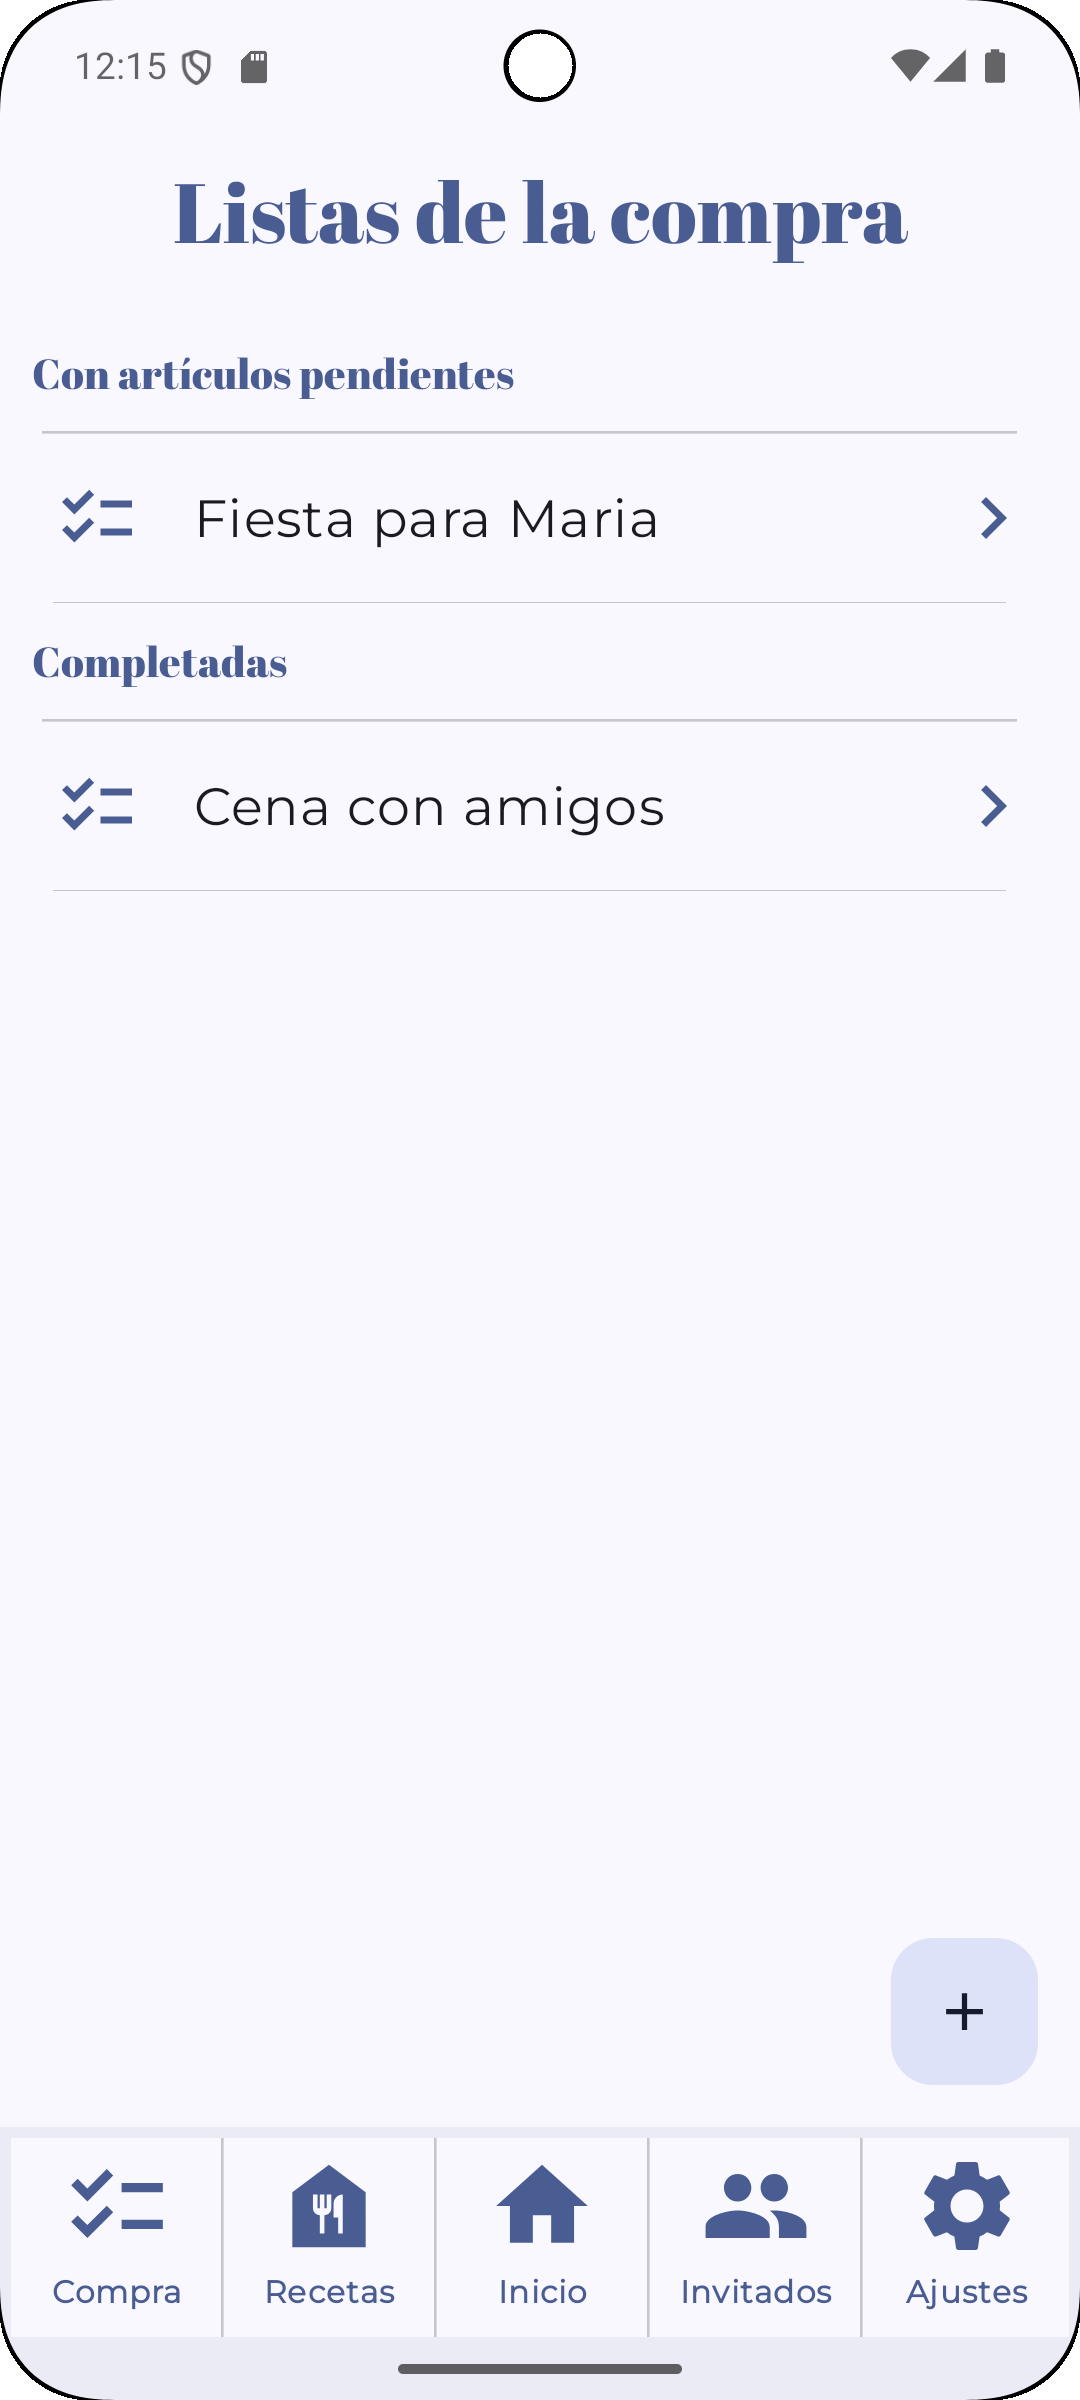
\includegraphics[width=\textwidth]{./img/manual/shopping_lists_with_all_items_bought_or_not.png}
      \caption{Completadas y pendientes}
      \label{fig:complete-or-not-shopping}
    \end{subfigure}

    \caption{Listas de la compra}
    \label{fig:shopping-lists}
\end{figure}

El usuario podrá crear listas de la compra desde la pantalla de crear lista Figura~\ref{fig:create-shopping}. Será obligatorio que añada un nombre a la lista Figura~\ref{fig:create-shopping-name}.

\begin{figure}[H]
    \centering

    \begin{subfigure}[b]{0.3\textwidth}
      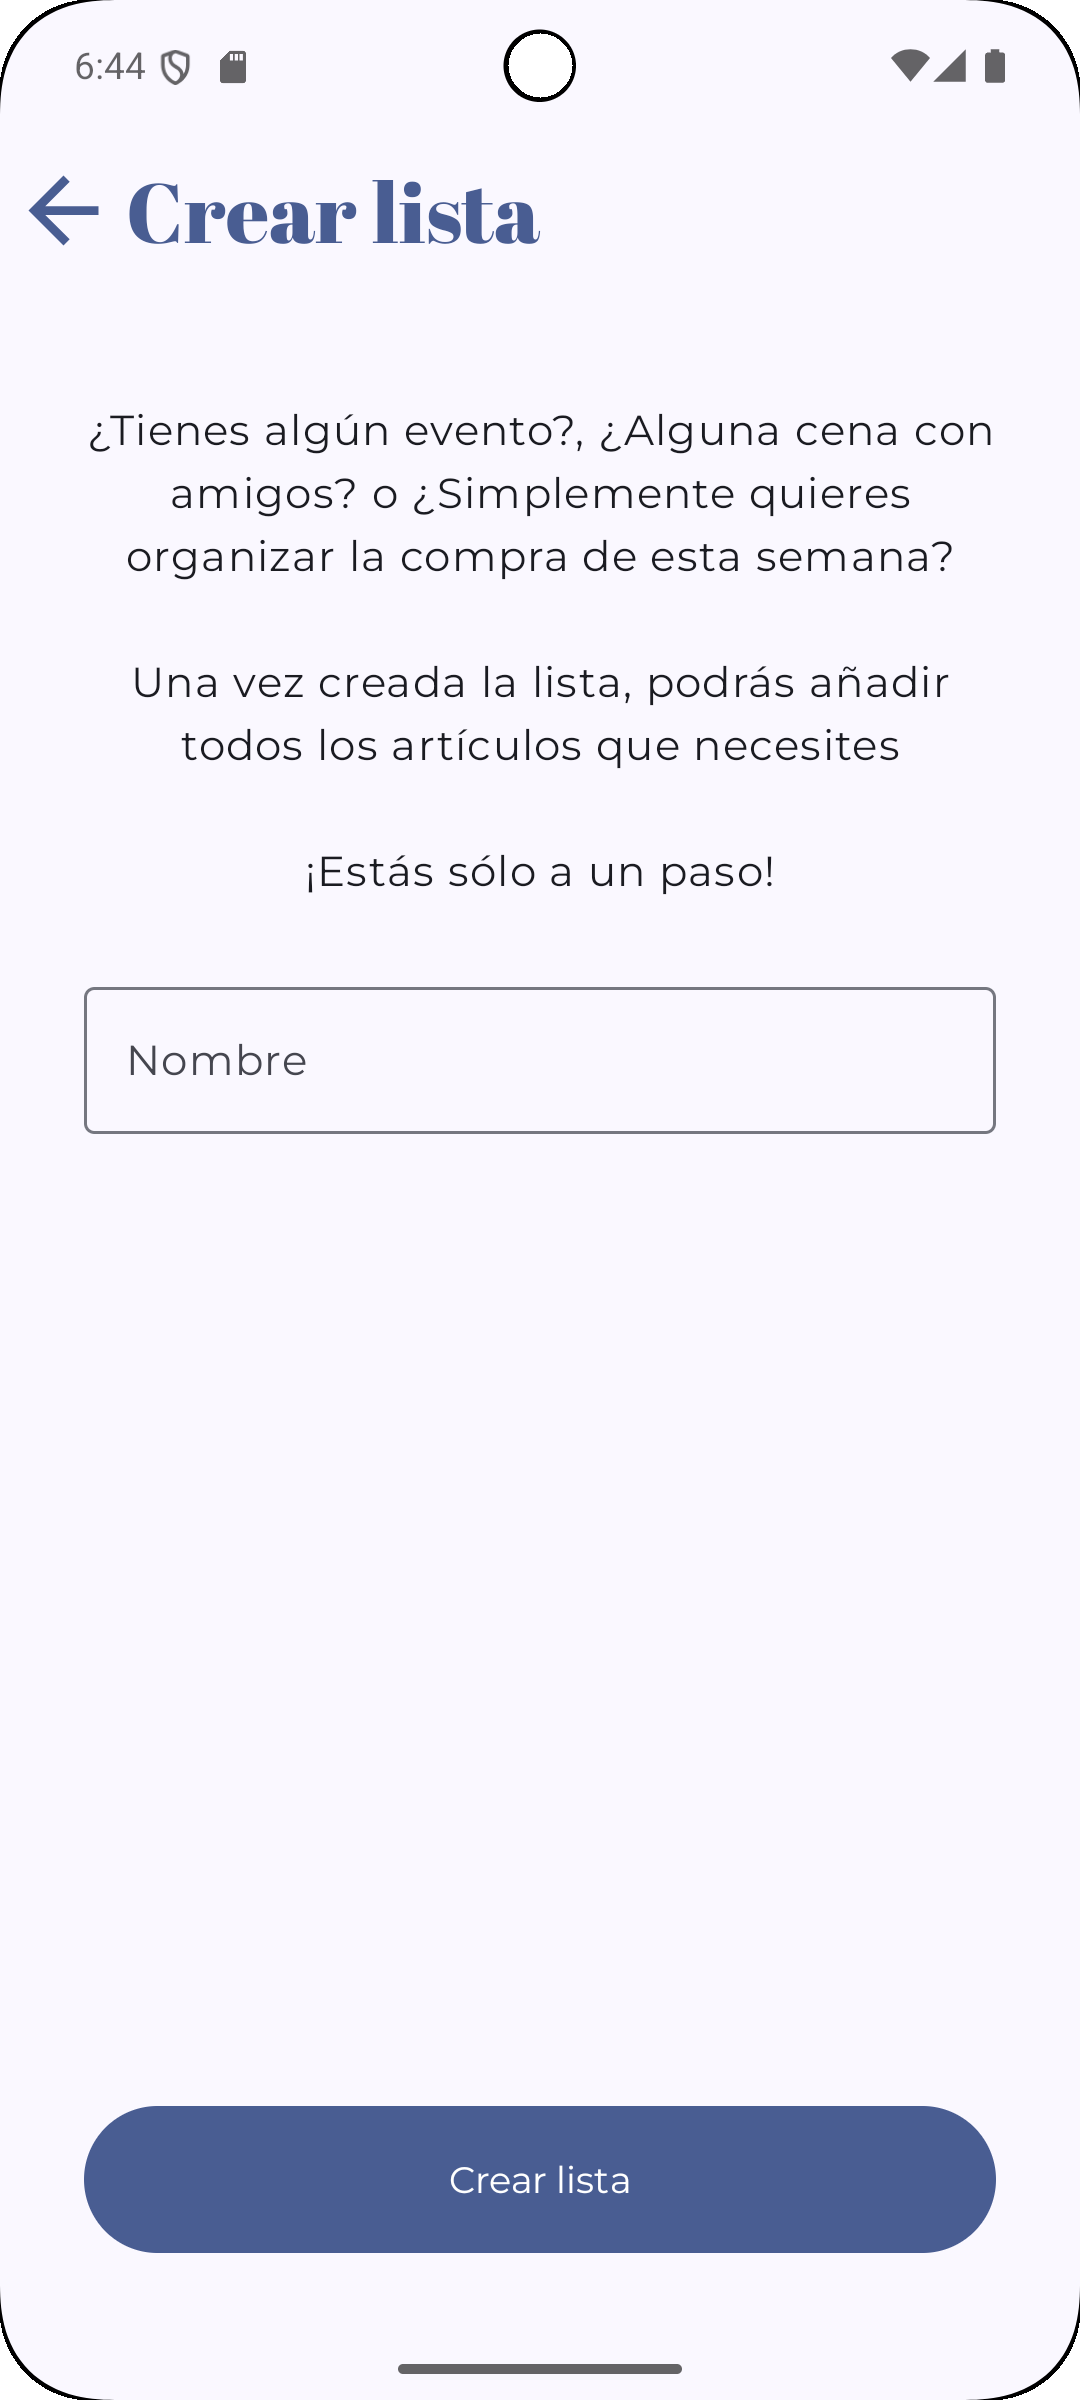
\includegraphics[width=\textwidth]{./img/manual/pinche_create_list.png}
      \caption{Pantalla de crear lista de la compra}
      \label{fig:create-shopping}
    \end{subfigure}
    \hfill
    \begin{subfigure}[b]{0.3\textwidth}
      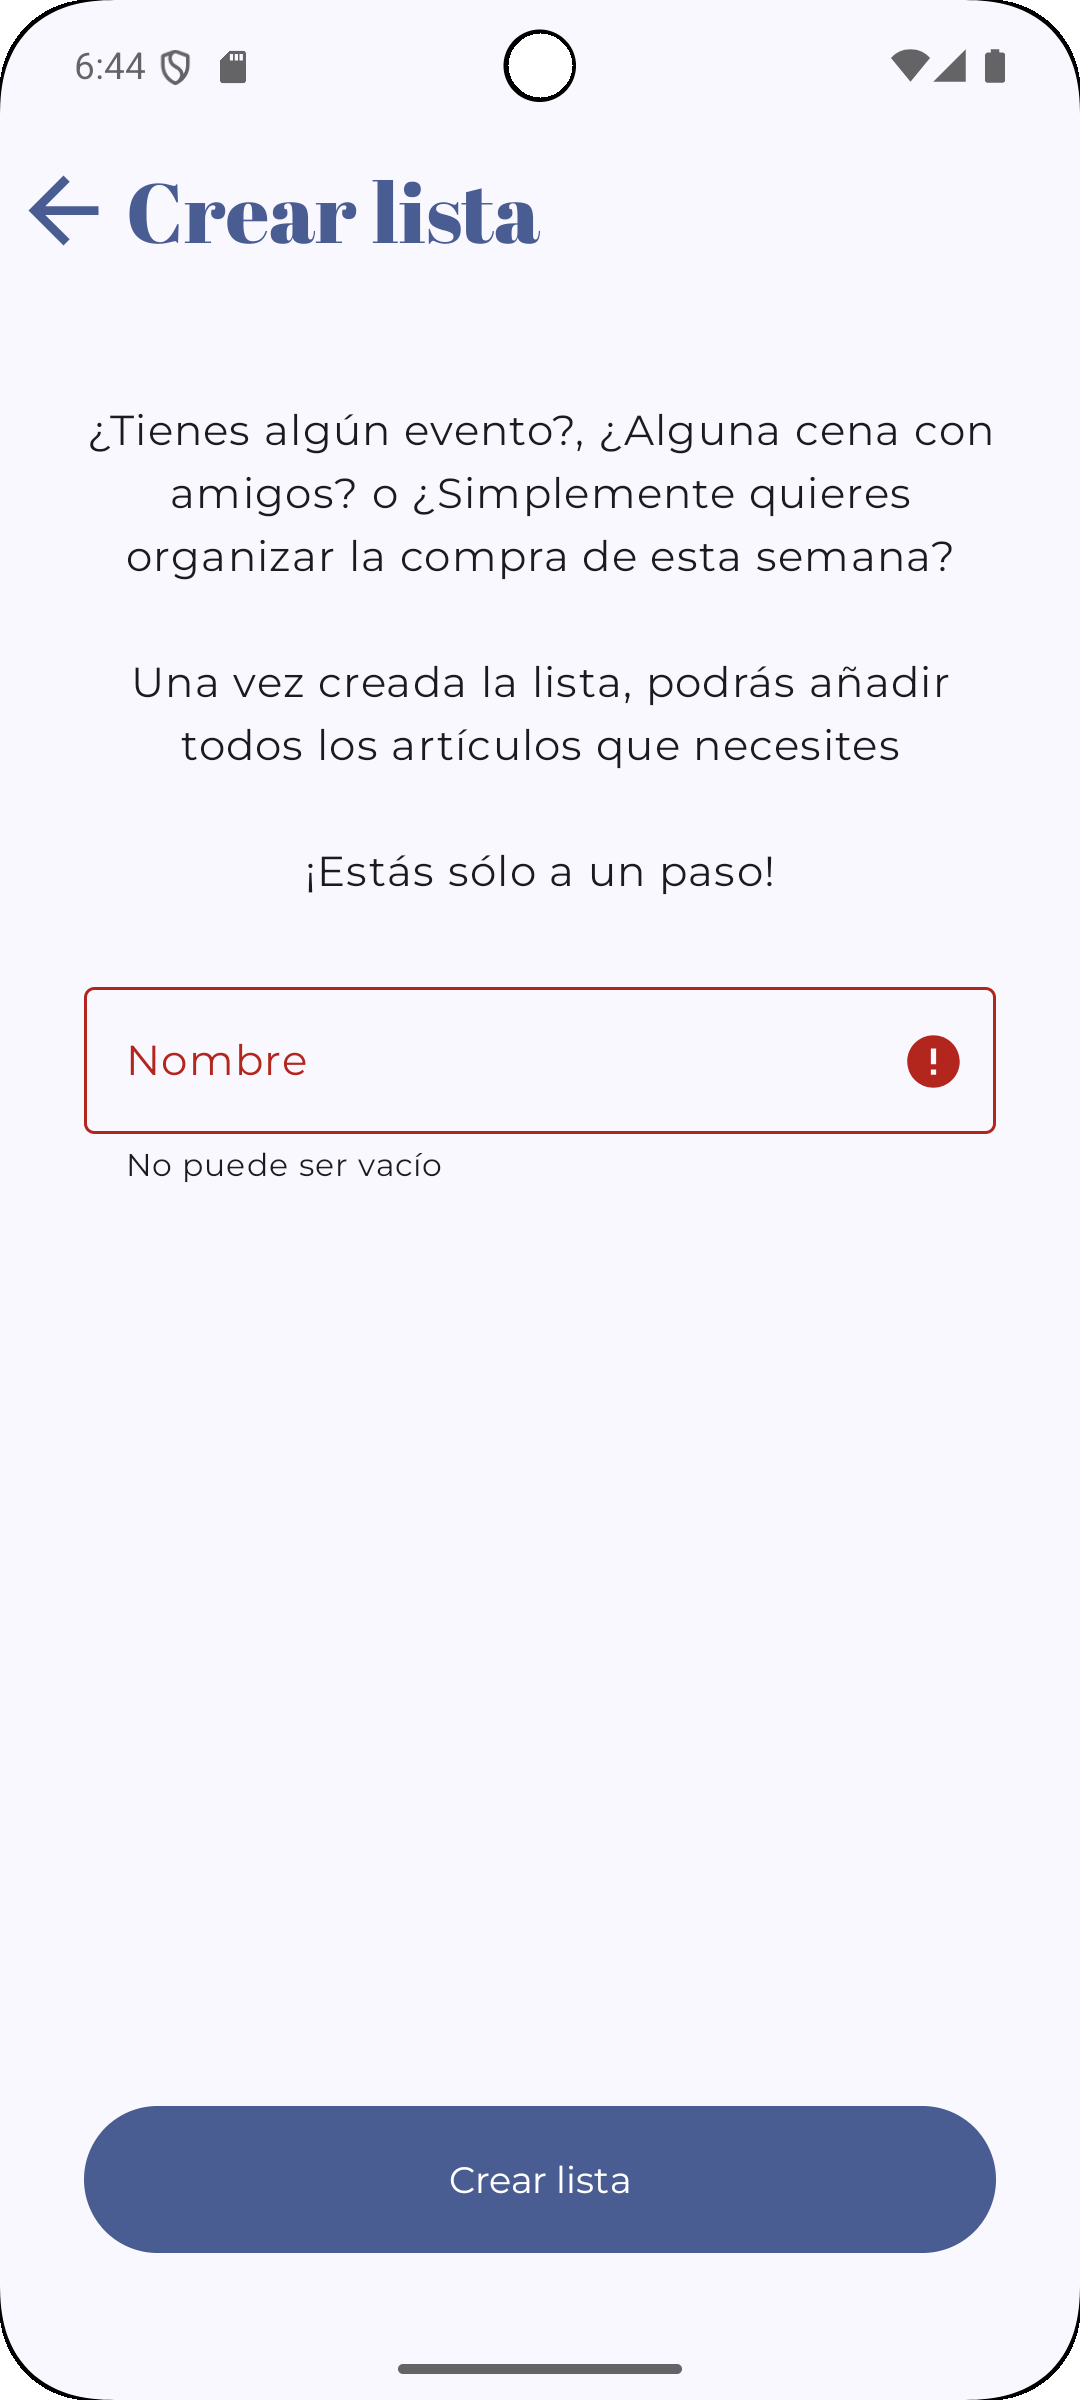
\includegraphics[width=\textwidth]{./img/manual/pinche_create_list_empty_name.png}
      \caption{Campo nombre obligatorio para crear lista}
      \label{fig:create-shopping-name}
    \end{subfigure}

    \caption{Crear lista de la compra}
    \label{fig:create-list}
\end{figure}

\clearpage
También podrá acceder al detalle de una lista, si la lista aún no tiene artículos se mostrará vacía Figura~\ref{fig:no-items}. Desde esta pantalla podrá eliminar una lista tras confirmar la acción Figura~\ref{fig:confirm-delete-list} o cambiar el nombre una lista Figura~\ref{fig:change-list-name}.

\begin{figure}[H]
    \centering

    \begin{subfigure}[b]{0.3\textwidth}
      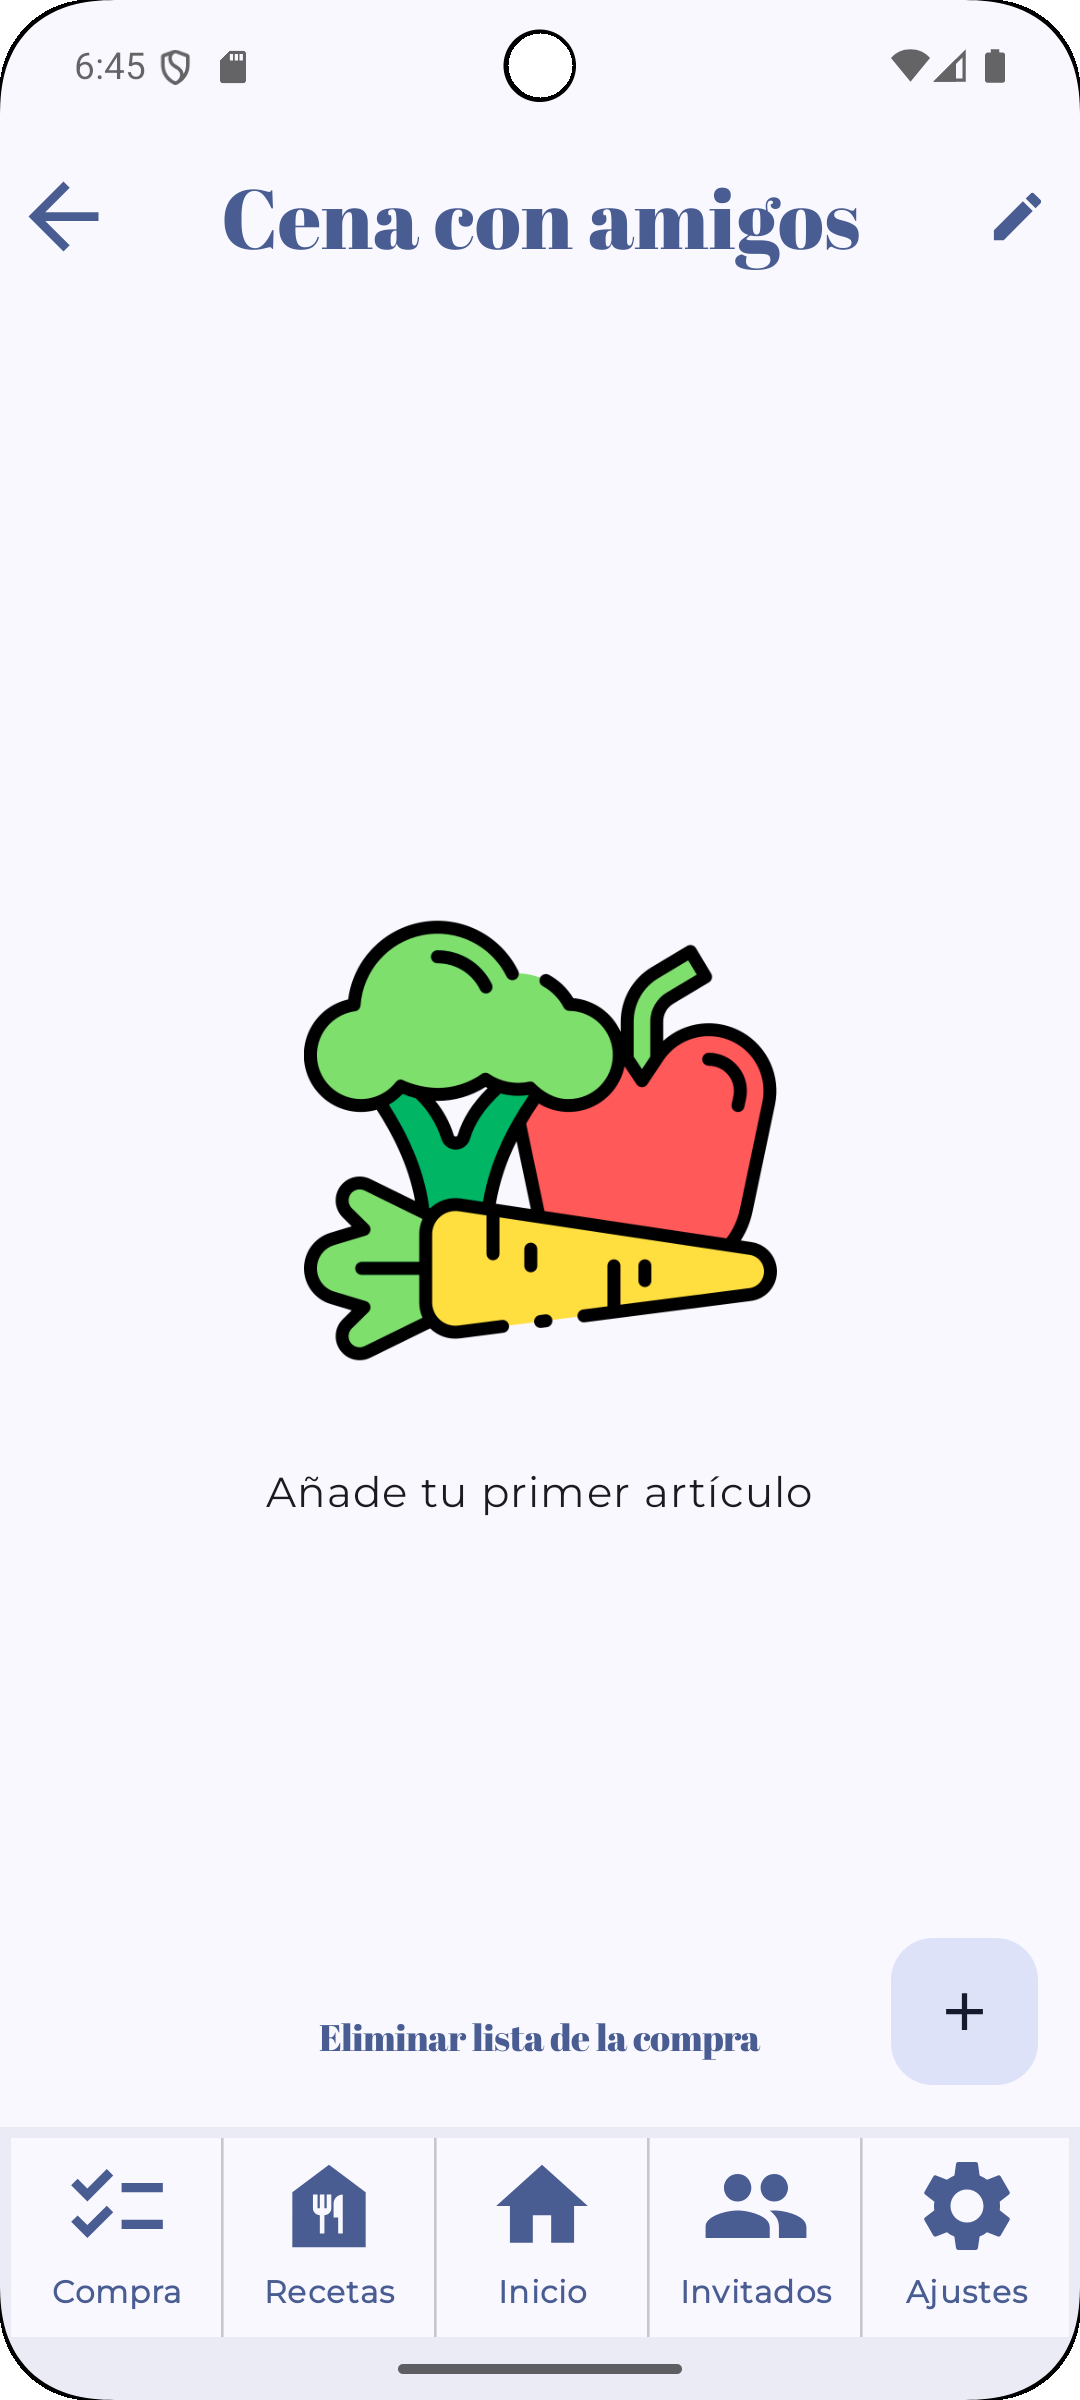
\includegraphics[width=\textwidth]{./img/manual/pinche_shopping_list_empty_items.png}
      \caption{Pantalla vacía de artículos}
      \label{fig:no-items}
    \end{subfigure}
    \hfill
    \begin{subfigure}[b]{0.3\textwidth}
      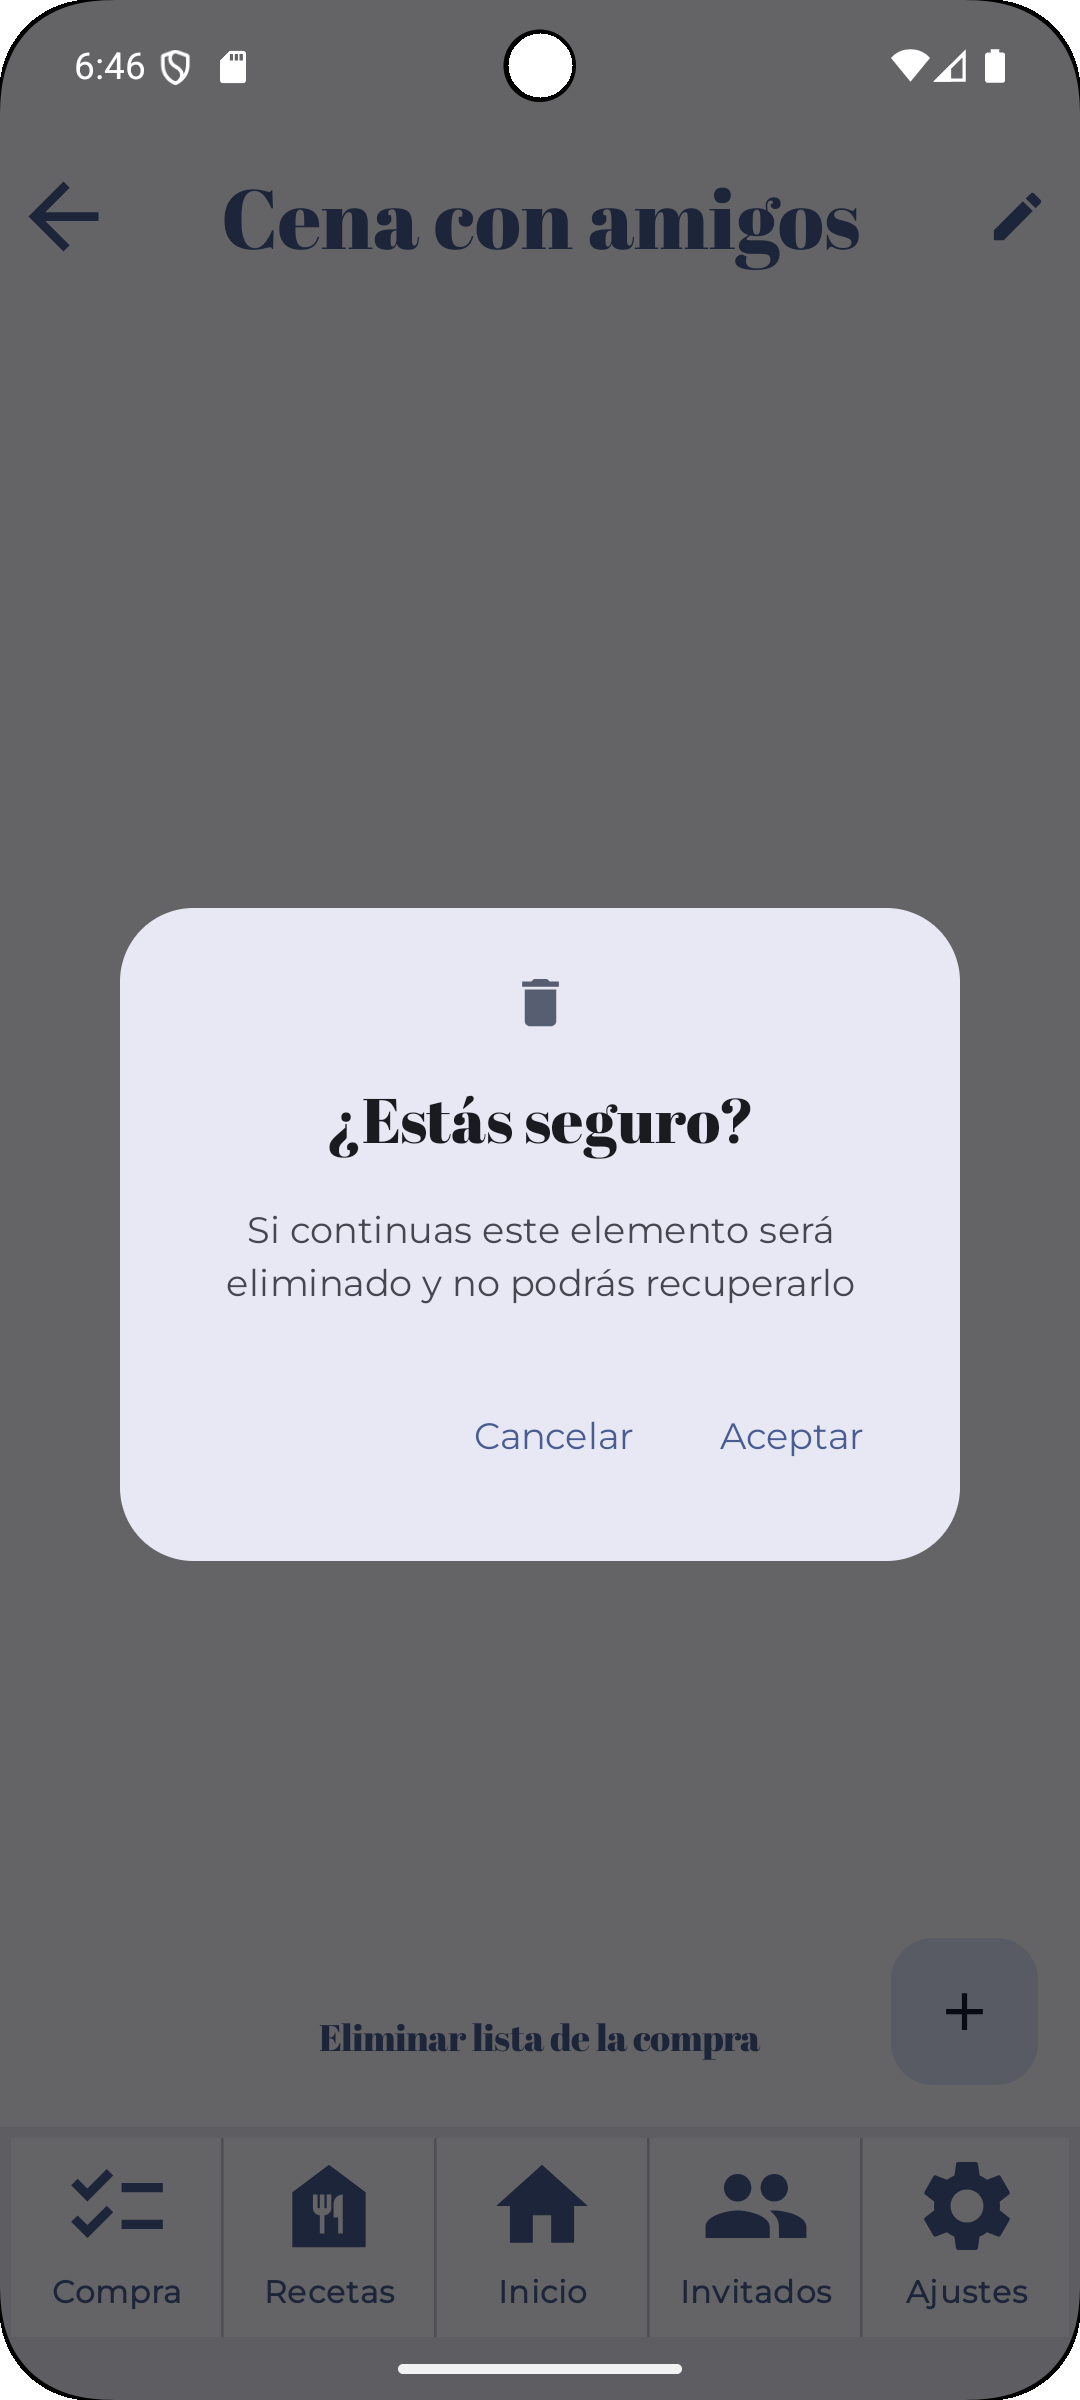
\includegraphics[width=\textwidth]{./img/manual/delete_shopping_list_confirm.png}
      \caption{Eliminar lista de la compra}
      \label{fig:confirm-delete-list}
    \end{subfigure}
    \hfill
    \begin{subfigure}[b]{0.3\textwidth}
      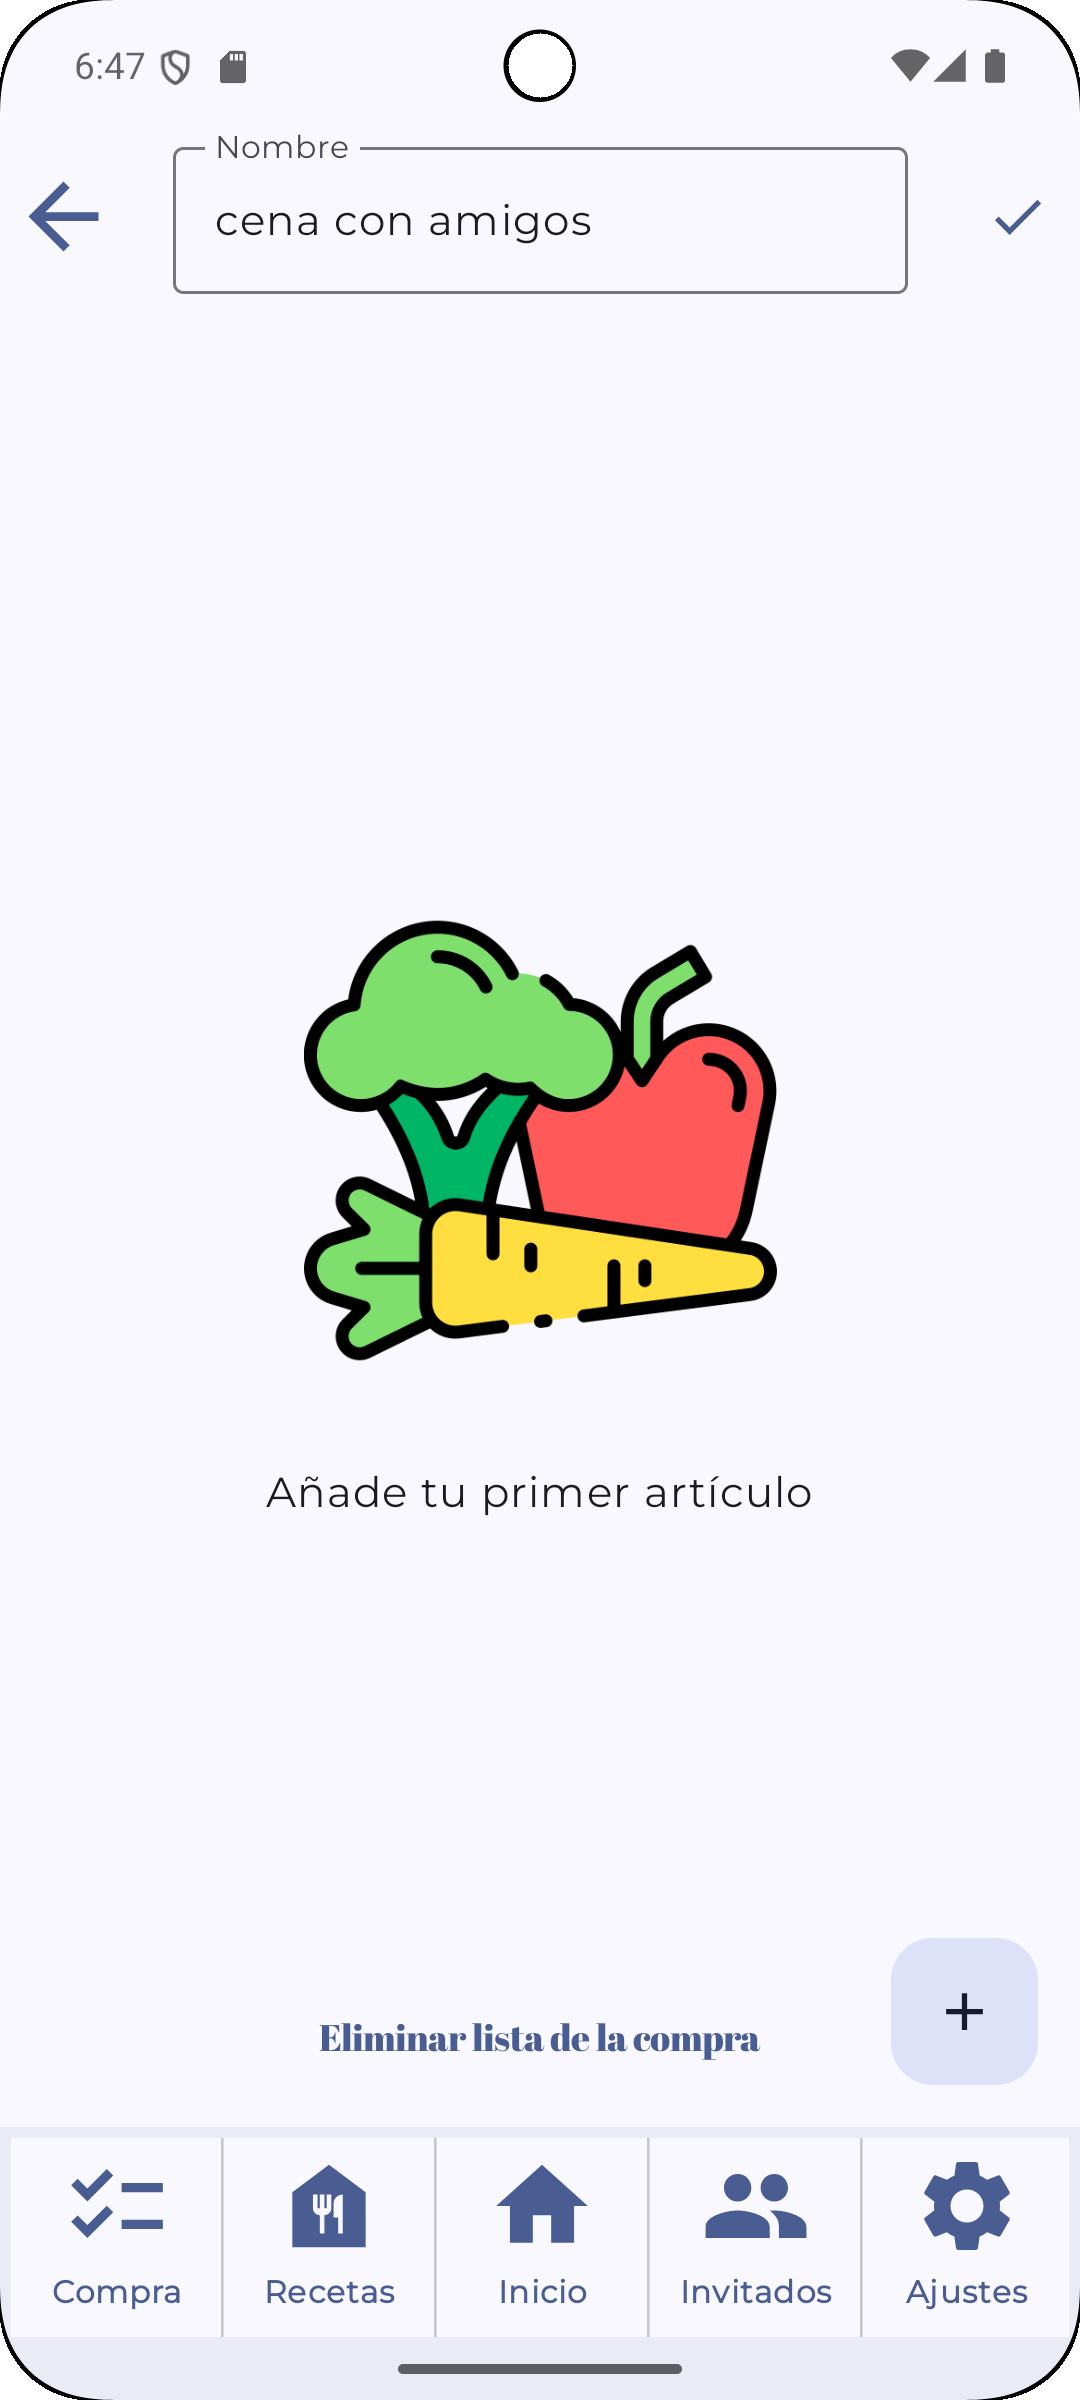
\includegraphics[width=\textwidth]{./img/manual/edit_shopping_list_name.png}
      \caption{Editar nombre de una lista}
      \label{fig:change-list-name}
    \end{subfigure}

    \caption{Detalle lista de la compra}
    \label{fig:shopping-lists-detail}
\end{figure}

Desde la pantalla del detalle de la lista de la compra el usuario puede añadir artículos con sus detalles Figura~\ref{fig:create-item}.

\begin{figure}[H]
    \centering

    \begin{subfigure}[b]{0.3\textwidth}
      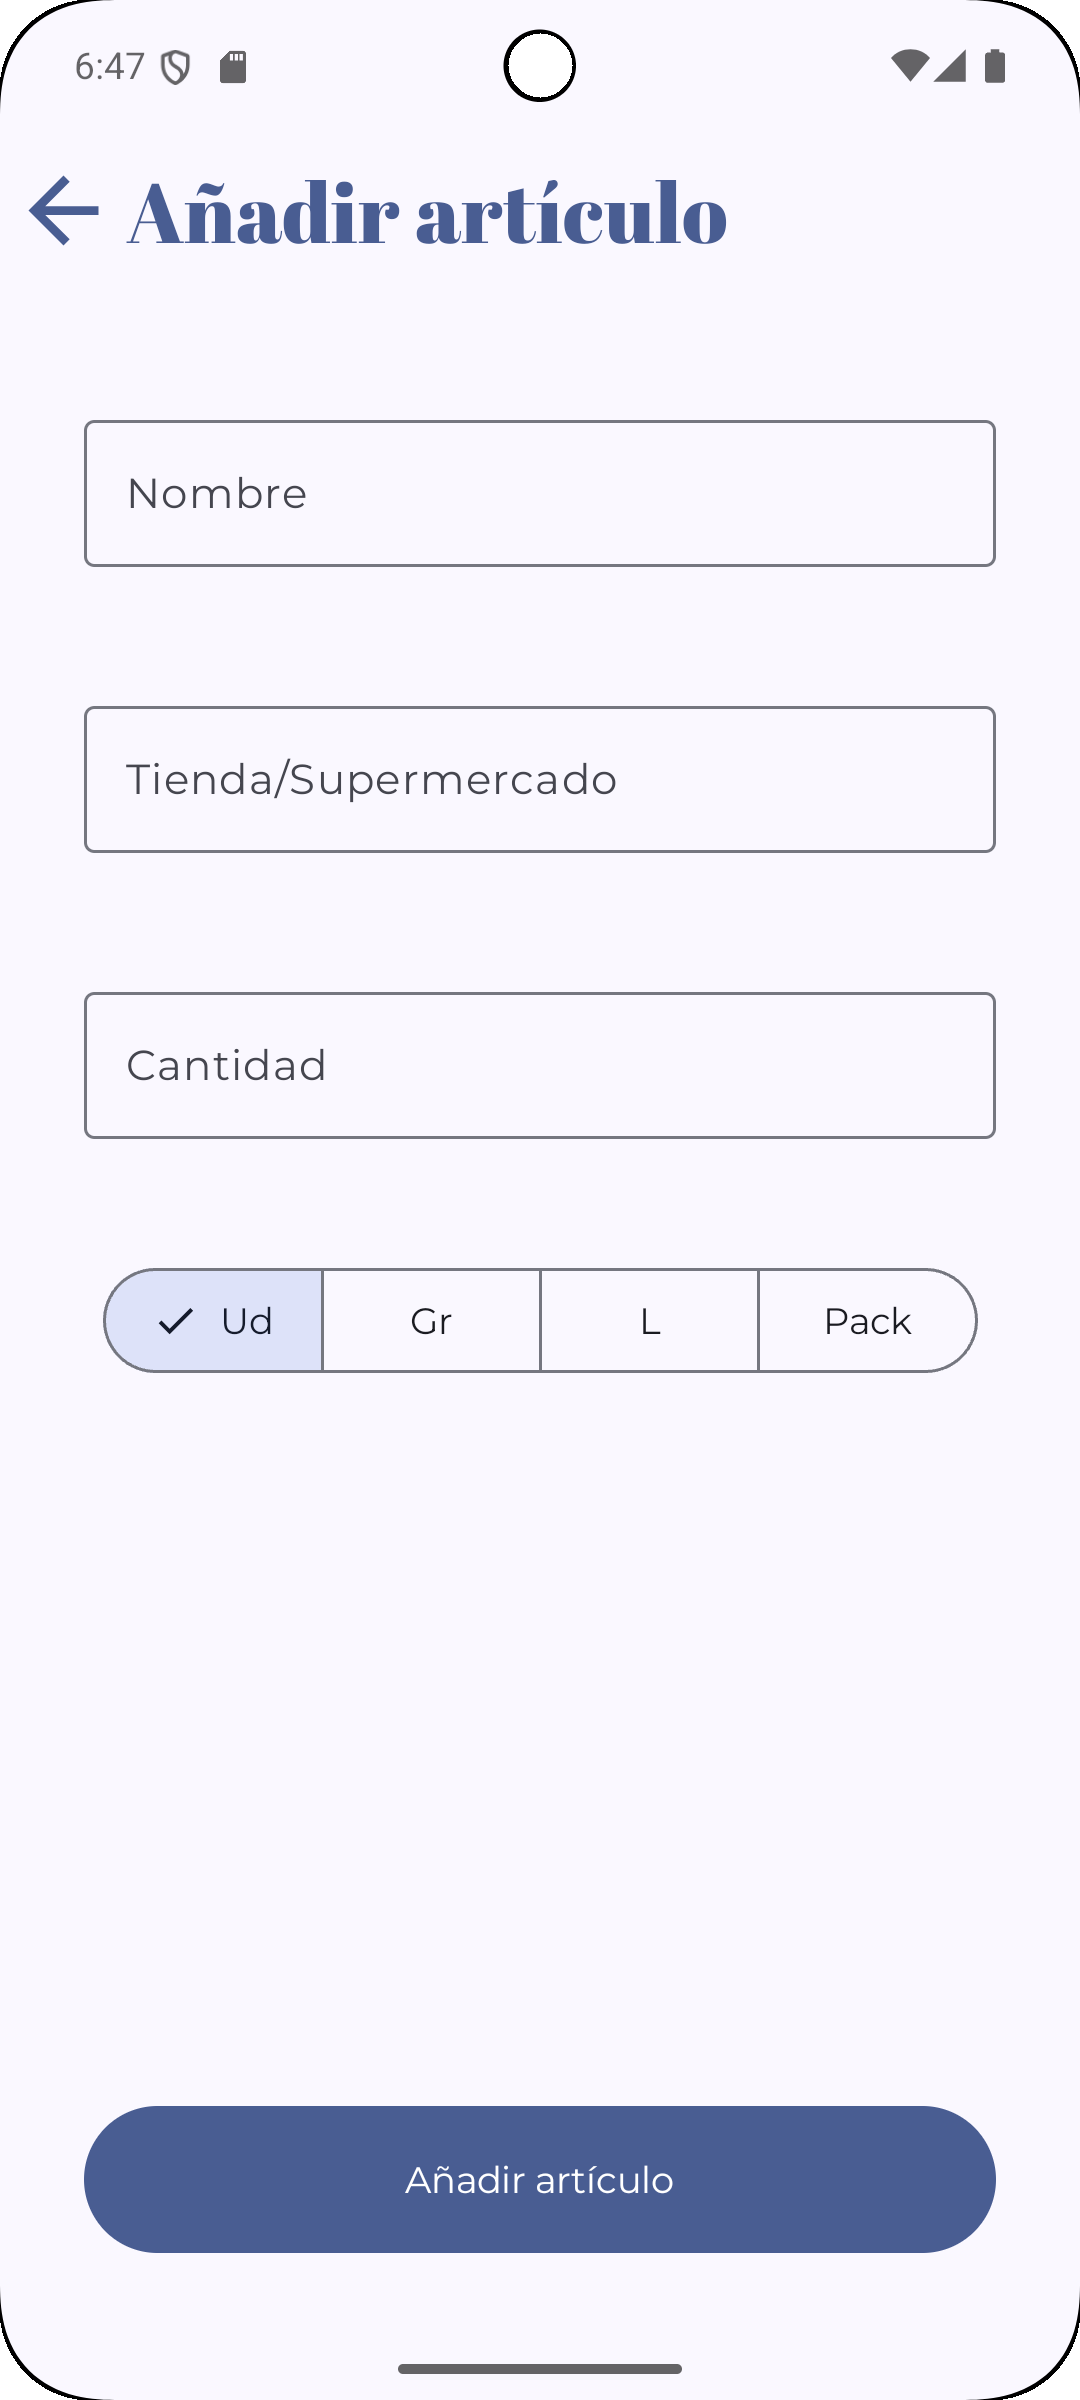
\includegraphics[width=\textwidth]{./img/manual/add_item_shopping_list.png}
      \caption{Detalles de un artículo}
      \label{fig:item-details}
    \end{subfigure}
    \hfill
    \begin{subfigure}[b]{0.3\textwidth}
      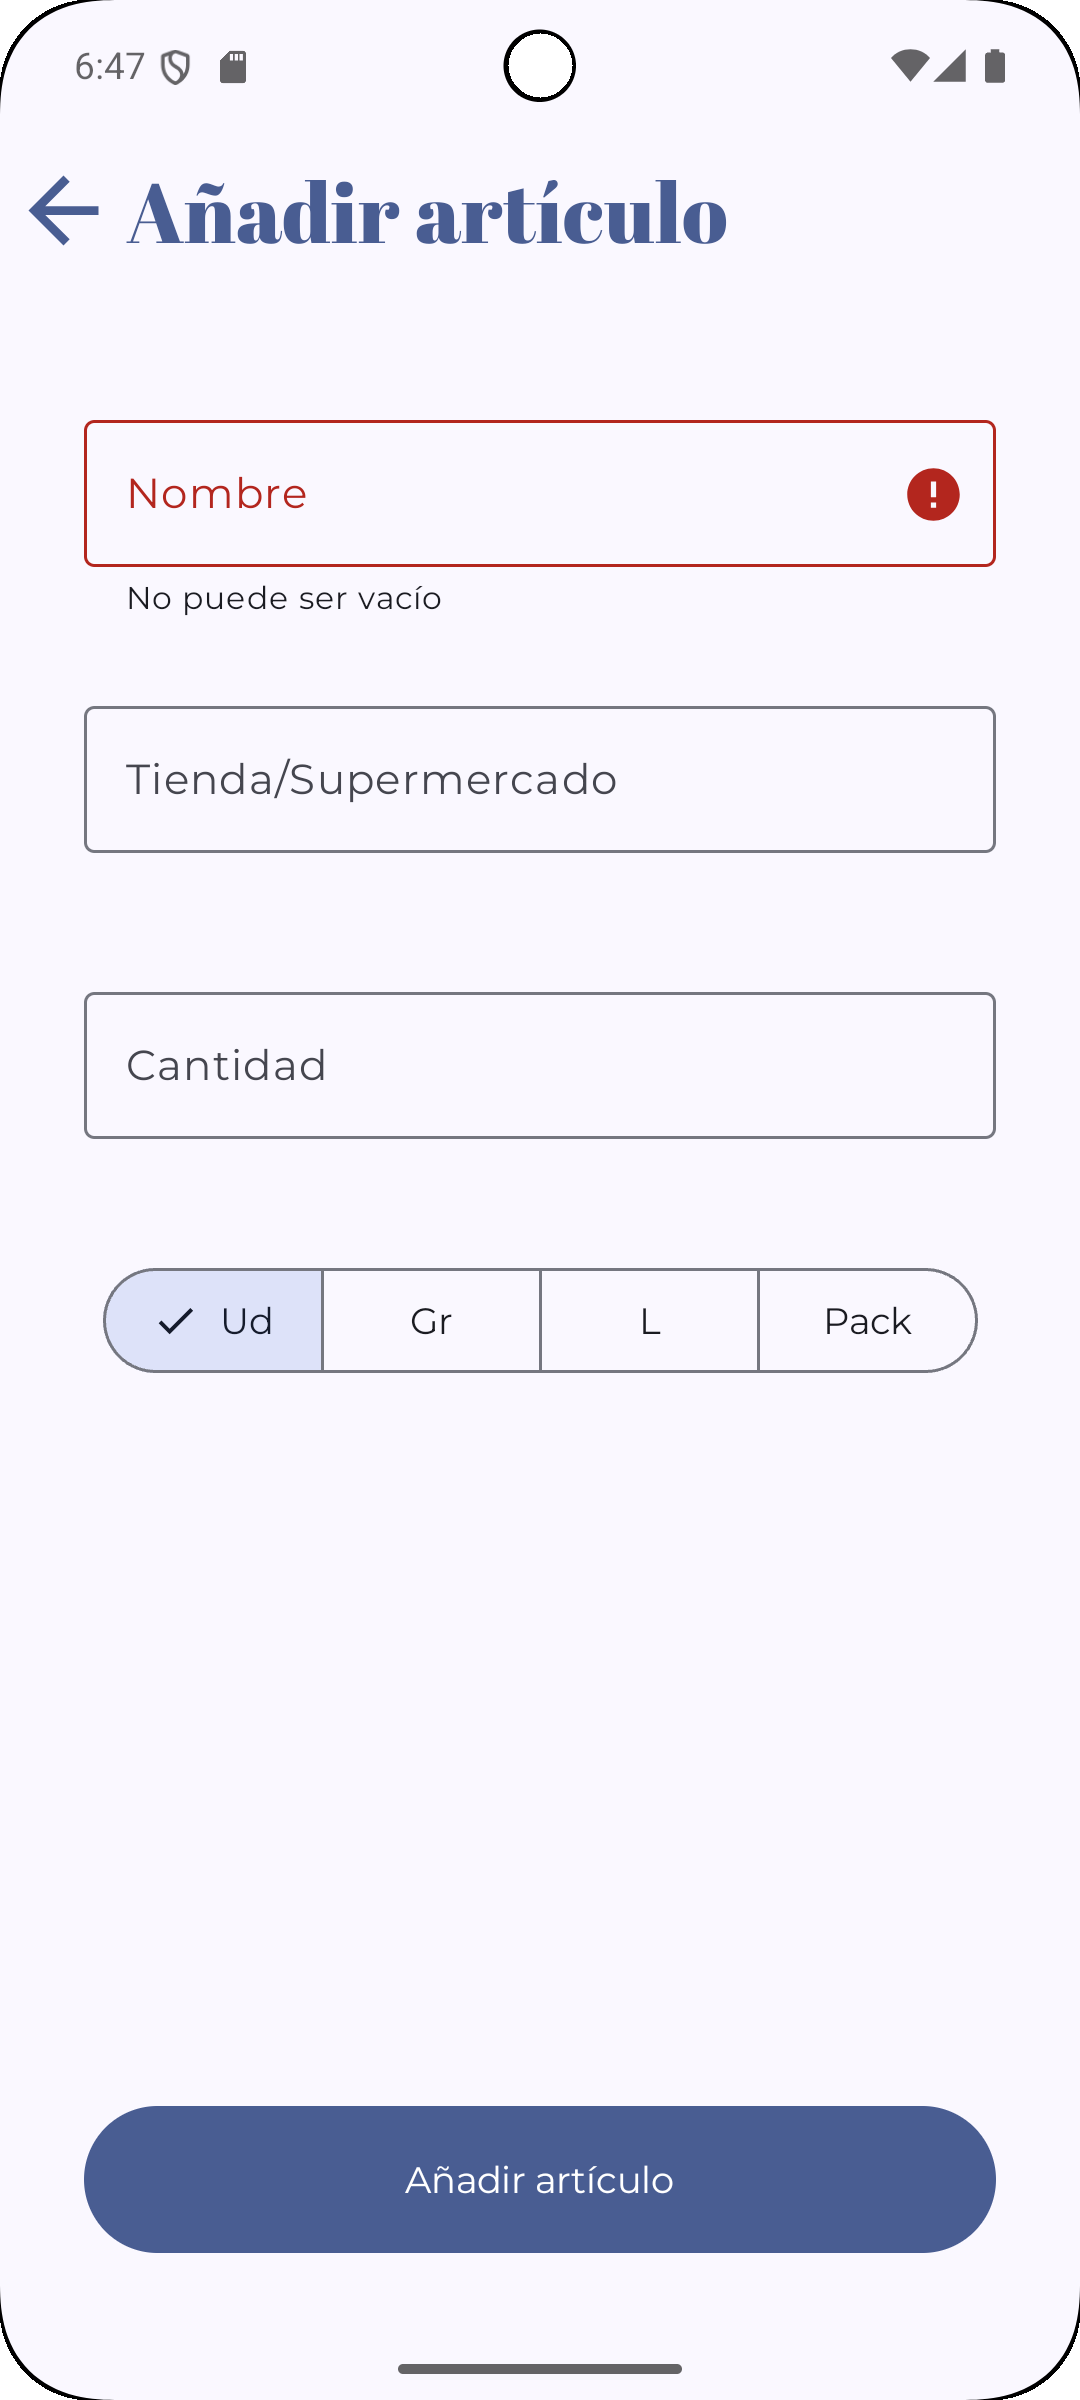
\includegraphics[width=\textwidth]{./img/manual/add_item_empty_name.png}
      \caption{Campo obligatorio}
      \label{fig:item-details-must}
    \end{subfigure}
    \hfill
    \begin{subfigure}[b]{0.3\textwidth}
      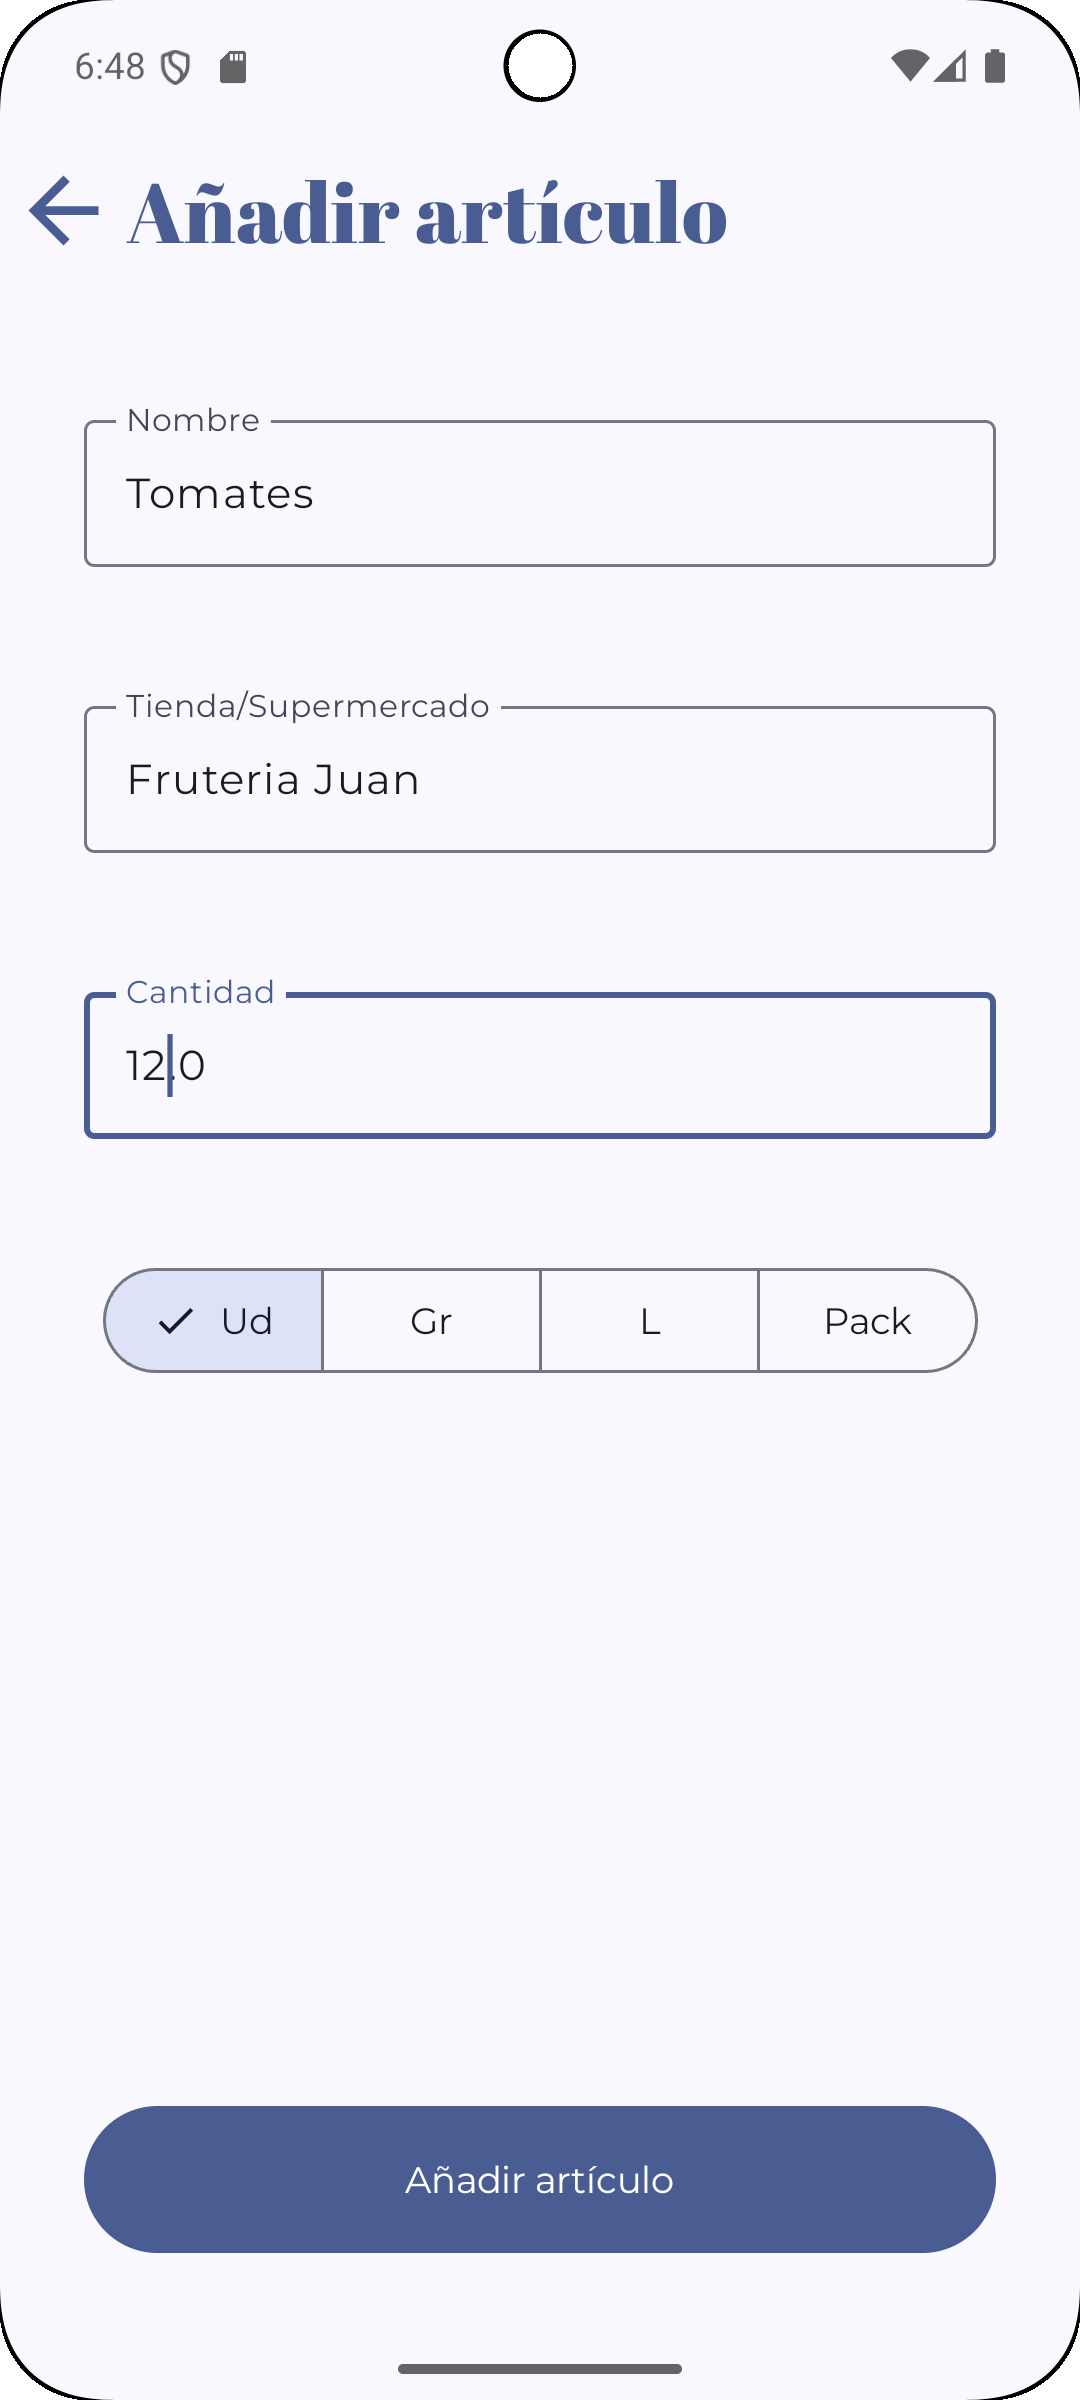
\includegraphics[width=\textwidth]{./img/manual/add_item_content_shopping_list.png}
      \caption{Añadir artículo}
      \label{fig:add-item}
    \end{subfigure}

    \caption{Añadir artículo}
    \label{fig:create-item}
\end{figure}

Una vez añadidos los artículos podrá visualizar los artículos de la lista, ver si están comprados o no, marcar todos como pendientes o marcar todos como comprados Figura~\ref{fig:items} y eliminarlos Figura~\ref{fig:delete-item}.

\begin{figure}[H]
    \centering

    \begin{subfigure}[b]{0.3\textwidth}
      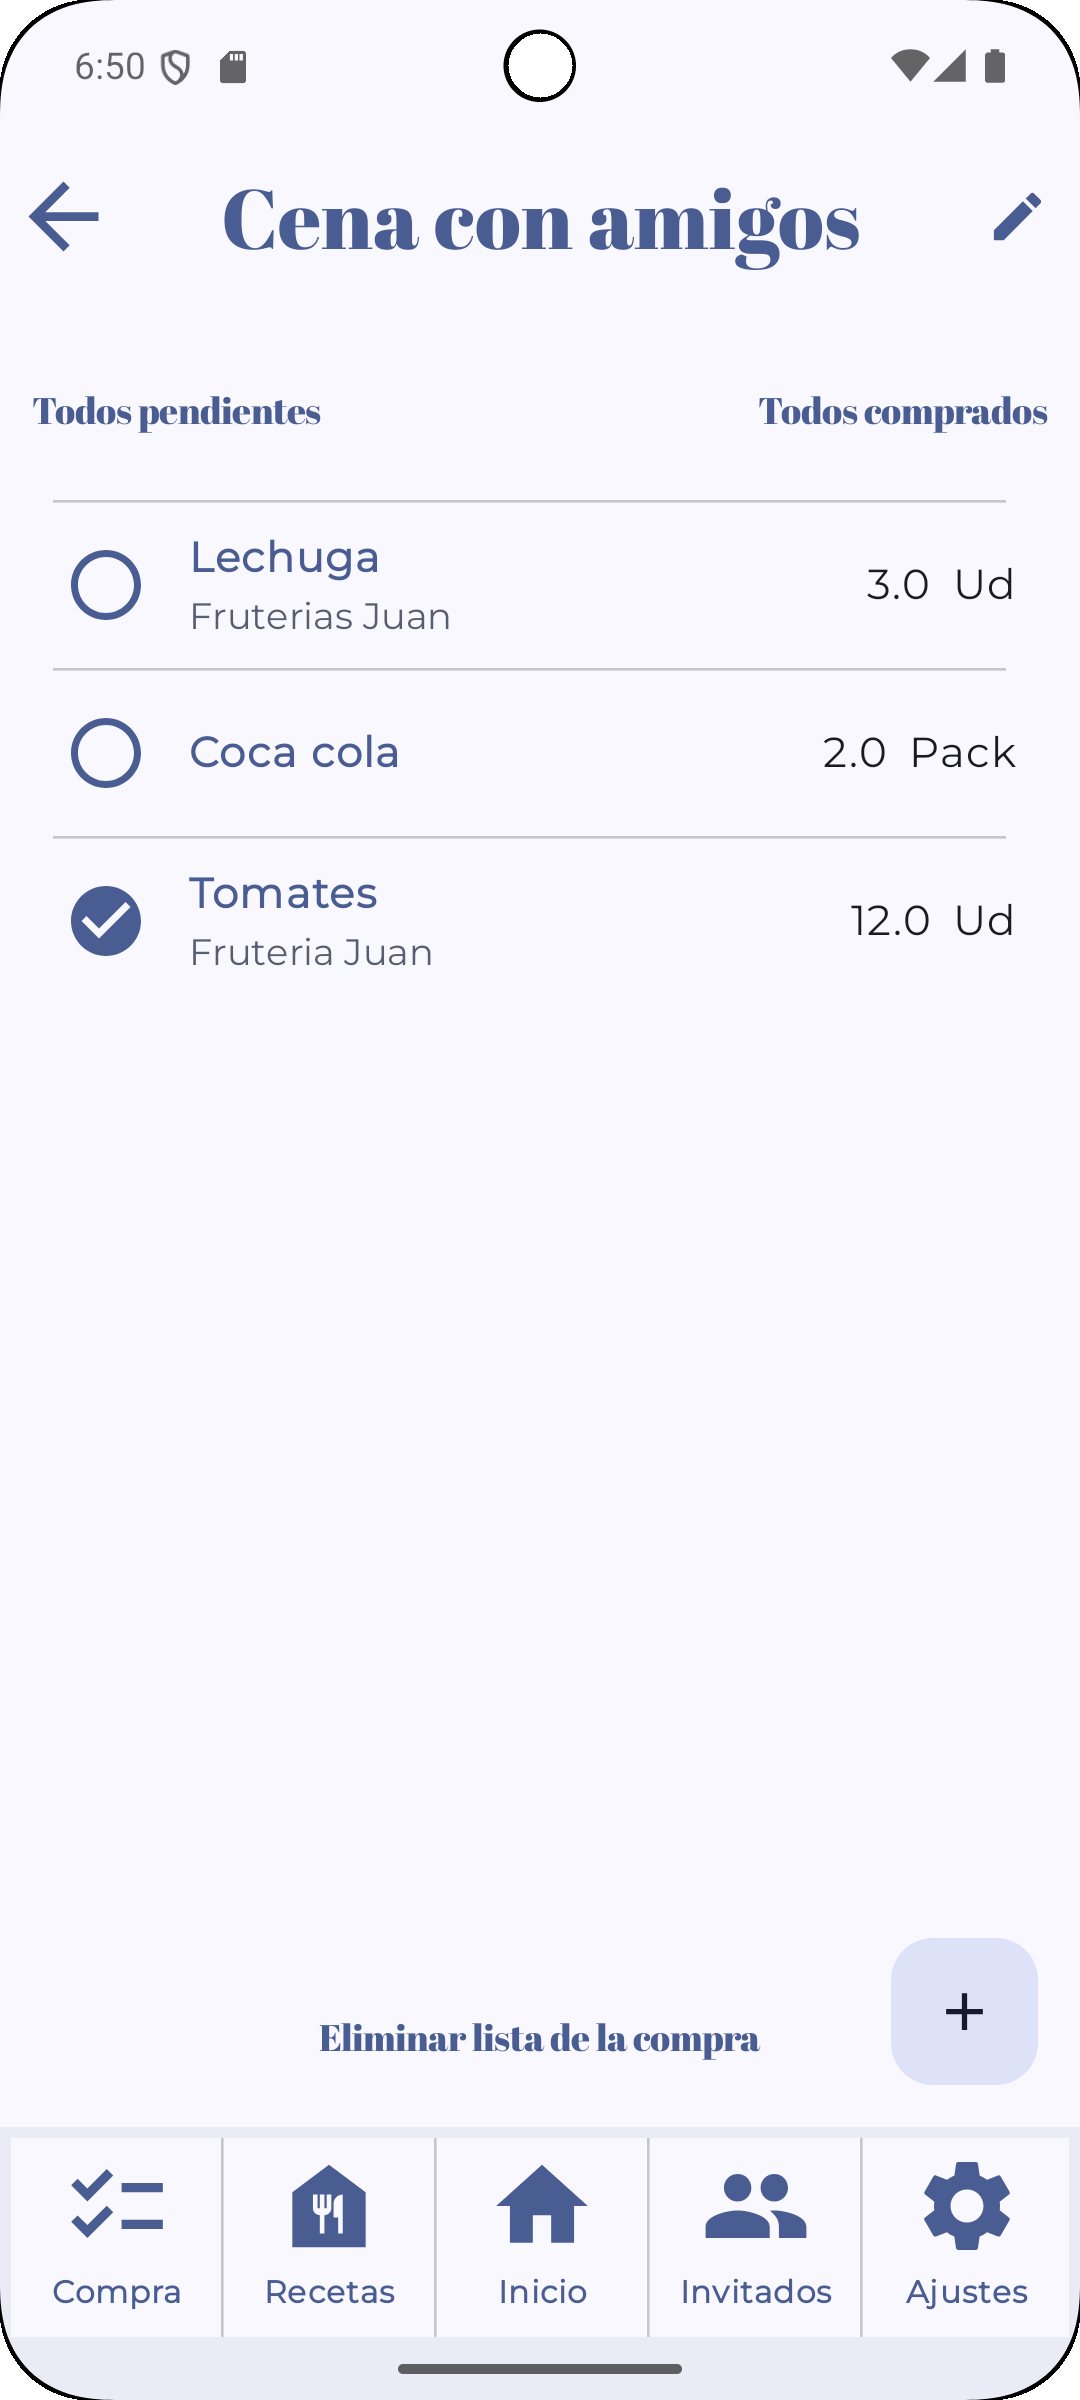
\includegraphics[width=\textwidth]{./img/manual/shopping_item_content.png}
      \caption{Lista de artículos}
      \label{fig:items}
    \end{subfigure}
    \hfill
    \begin{subfigure}[b]{0.3\textwidth}
      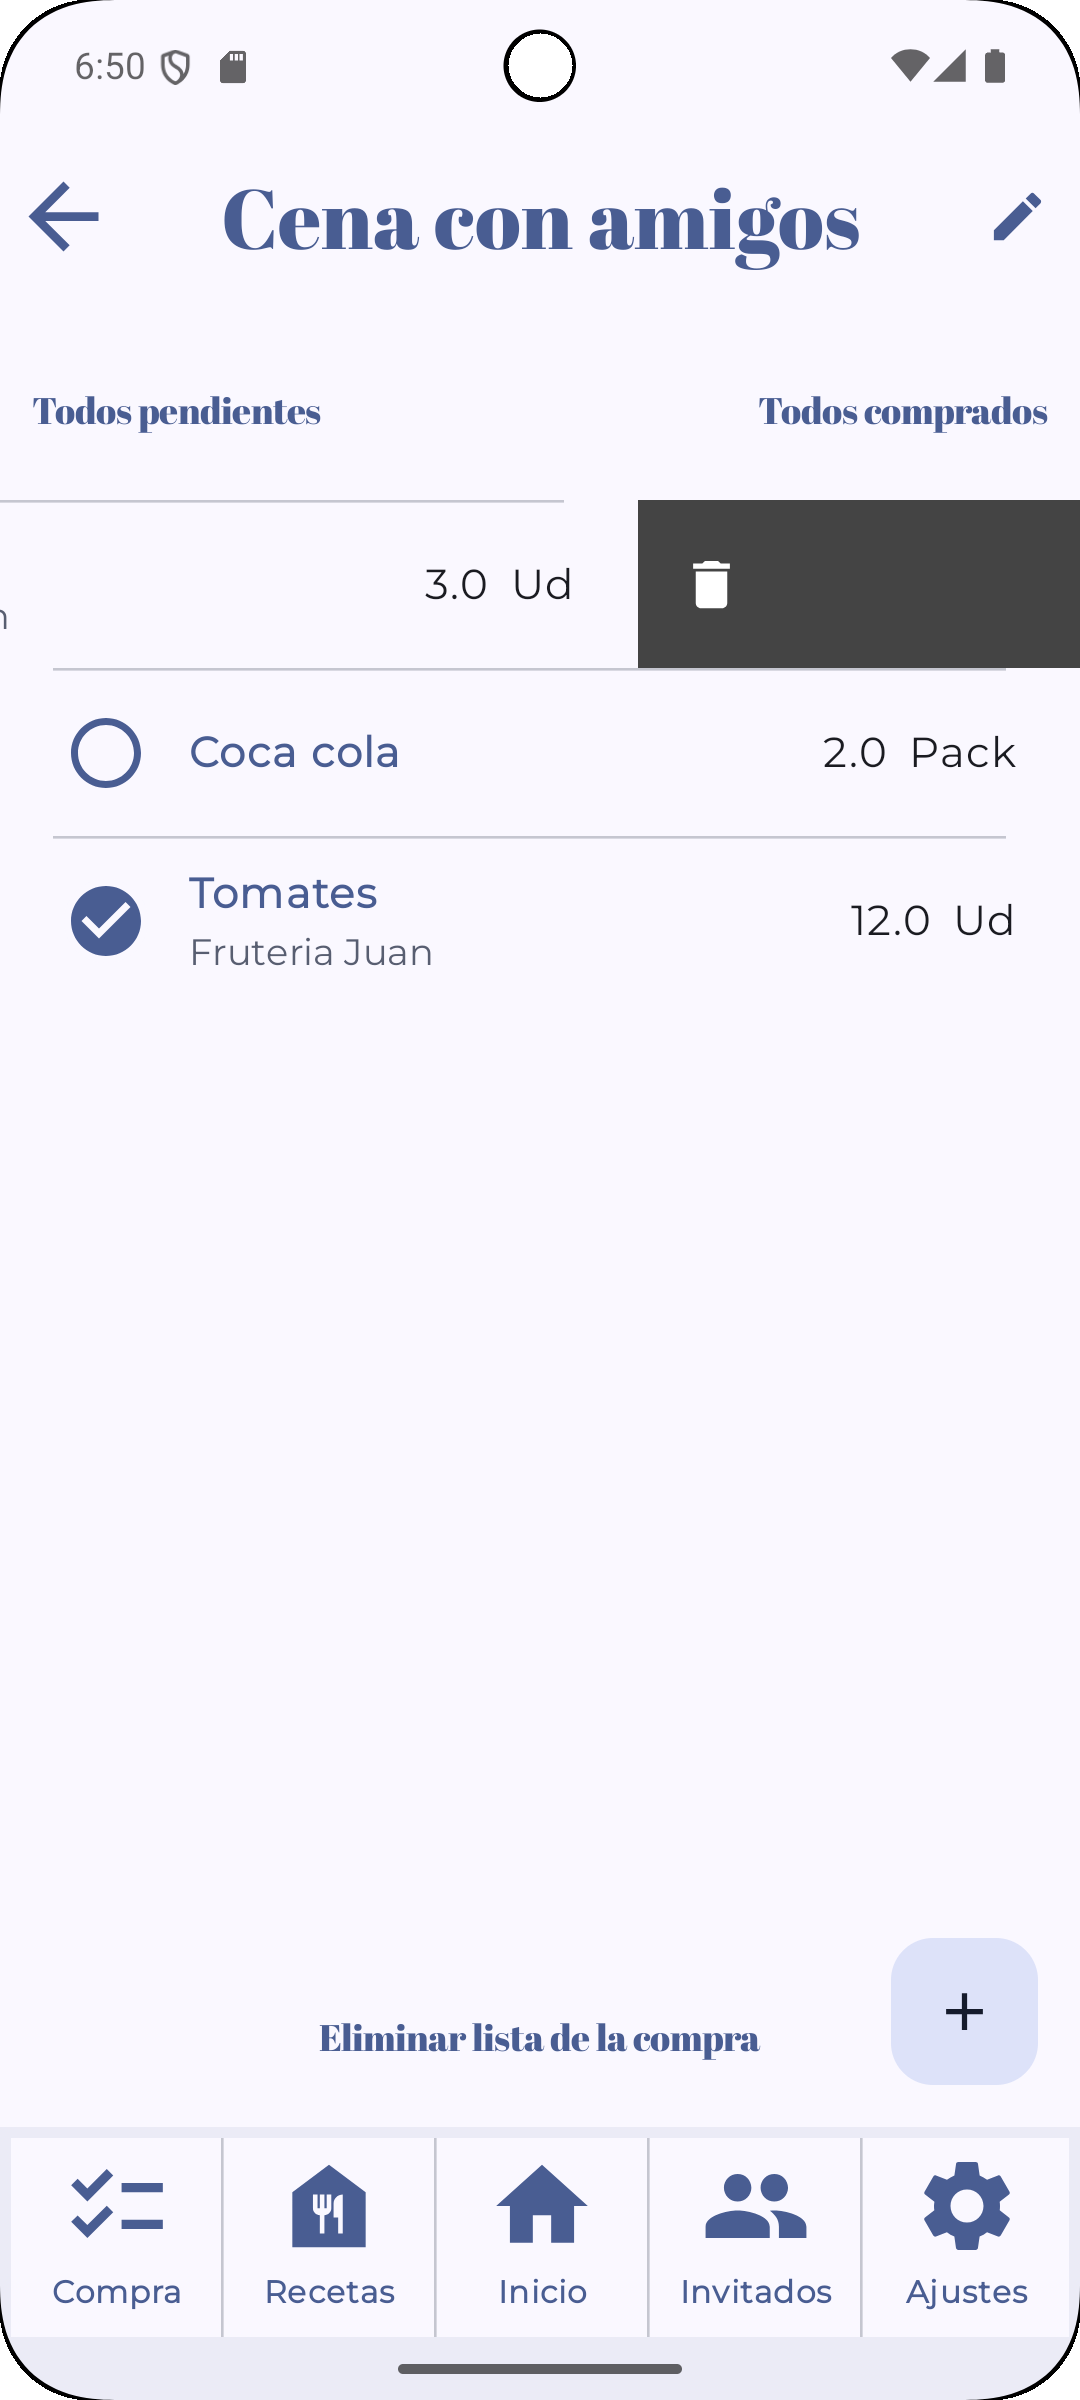
\includegraphics[width=\textwidth]{./img/manual/delete_item.png}
      \caption{Eliminar artículo}
      \label{fig:delete-item}
    \end{subfigure}

    \caption{Artículos}
    \label{fig:items-detail}
\end{figure}

%% recetas
\clearpage
Desde la pantalla principal también puede acceder a la sección de \textbf{recetas}. Si no hay recetas, se mostrará el estado de la pantalla de recetas vacía Figura~\ref{fig:recipes-empty}. En el caso de que sí haya recetas se le muestran al usuario Figura~\ref{fig:recipes-not-empty}. Desde aquí podrá añadir recetas, acceder al detalle de las recetas que ya ha añadido (falta por implementar) y eliminarlas tras confirmar la acción Figura~\ref{fig:delete-recipes}.

\begin{figure}[H]
    \centering

    \begin{subfigure}[b]{0.3\textwidth}
      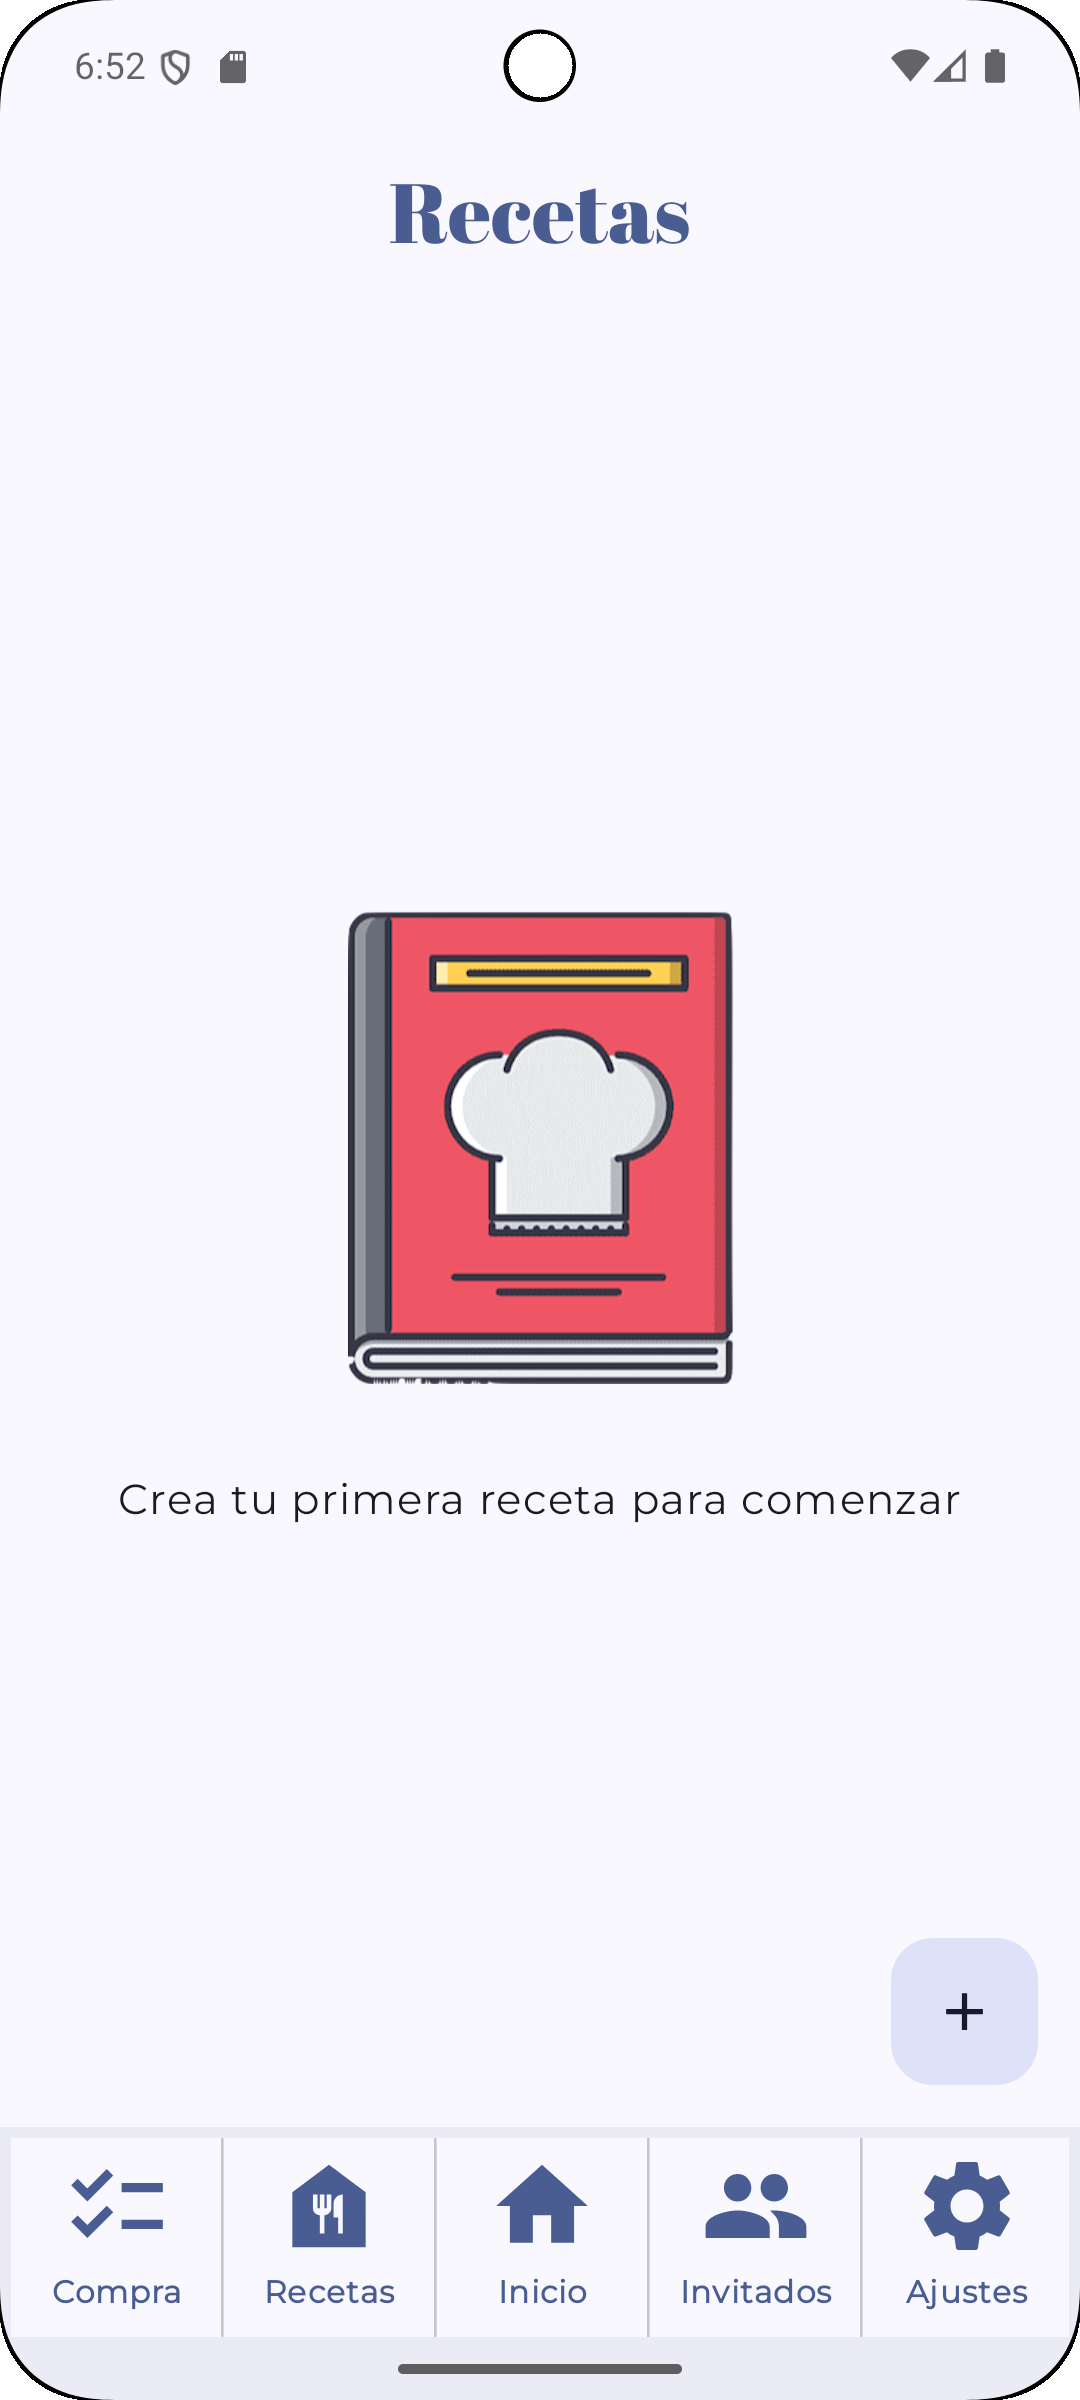
\includegraphics[width=\textwidth]{./img/manual/recipes_list_empty.png}
      \caption{Pantalla de recetas vacía}
      \label{fig:recipes-empty}
    \end{subfigure}
    \hfill
    \begin{subfigure}[b]{0.3\textwidth}
      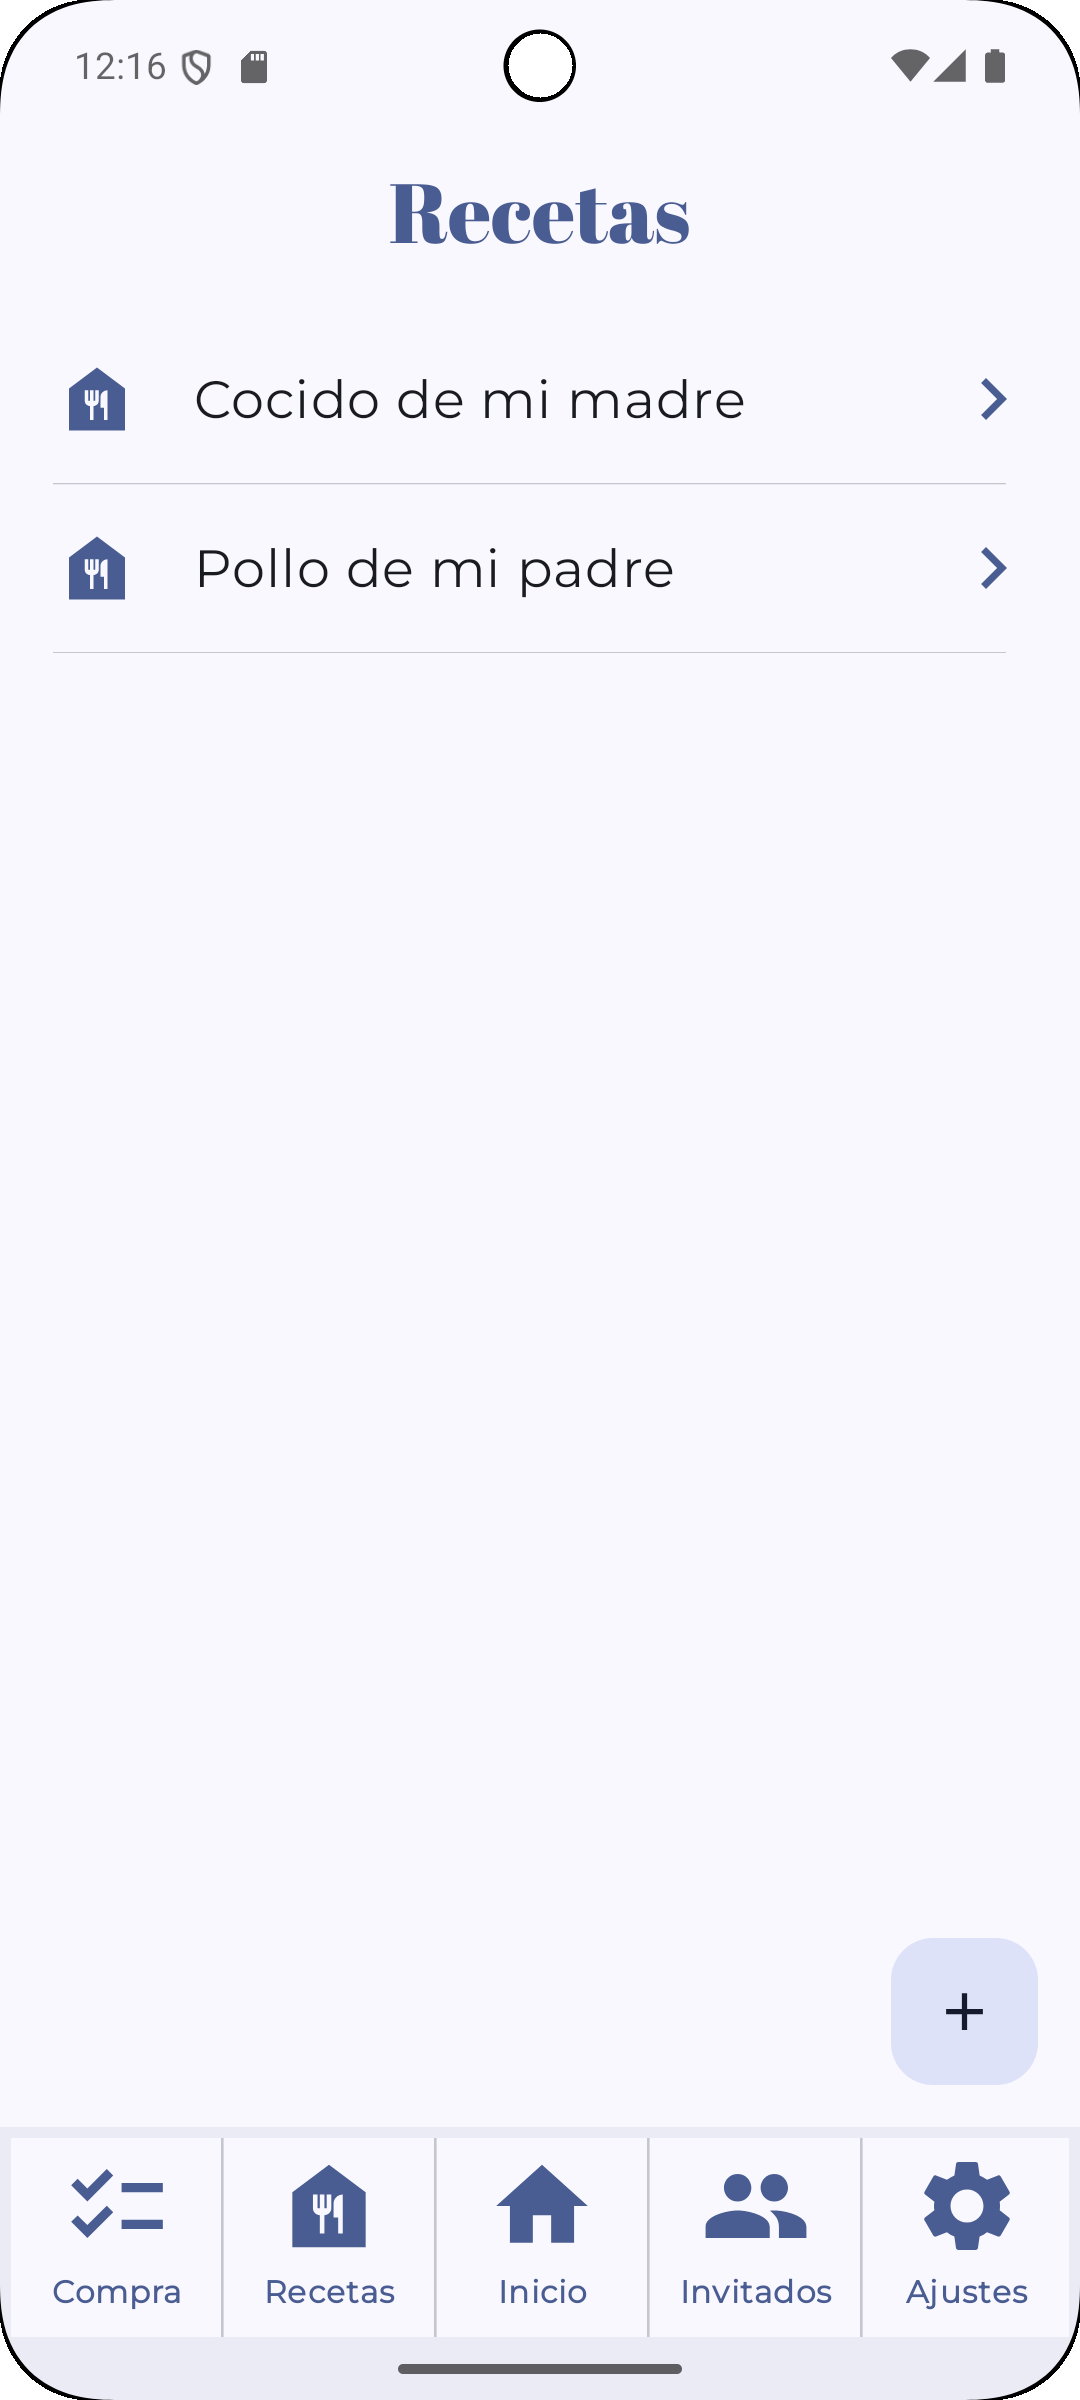
\includegraphics[width=\textwidth]{./img/manual/recipes_not_empty.png}
      \caption{Pantalla de recetas}
      \label{fig:recipes-not-empty}
    \end{subfigure}
    \hfill
    \begin{subfigure}[b]{0.3\textwidth}
      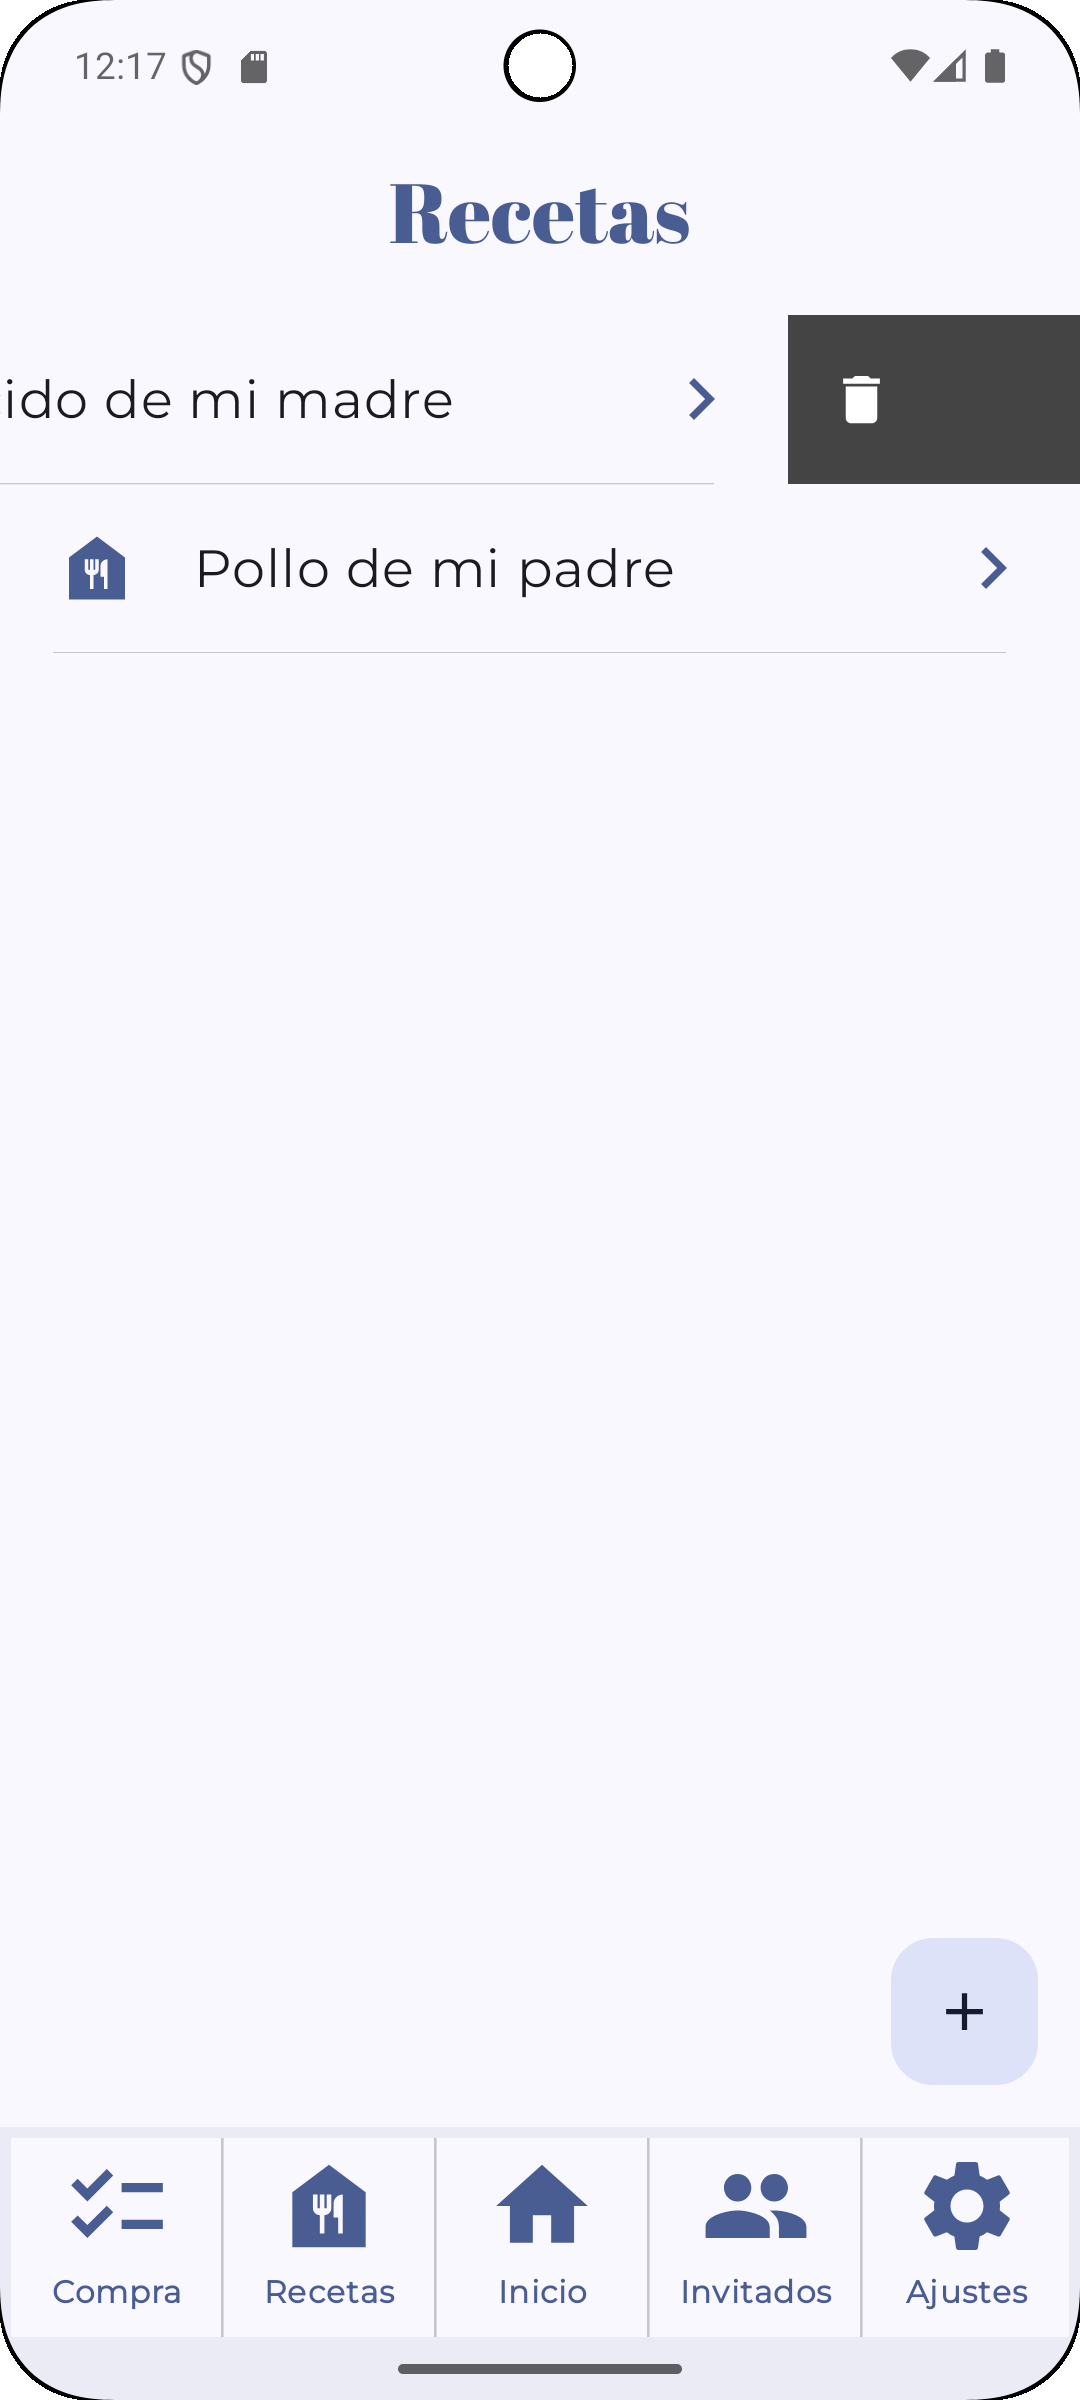
\includegraphics[width=\textwidth]{./img/manual/delete_recipe.png}
      \caption{Eliminar receta}
      \label{fig:delete-recipes}
    \end{subfigure}

    \caption{Recetas}
    \label{fig:recipes}
\end{figure}

%% invitados
\clearpage
Desde la pantalla principal también puede acceder a la sección de \textbf{invitados}. Si no hay invitados, se mostrará el estado de la pantalla de invitados vacía Figura~\ref{fig:guest-empty}. En el caso de que sí haya introducido invitados se le muestran al usuario Figura~\ref{fig:guest-not-empty}. Desde aquí podrá añadir invitados, acceder al detalle de los invitados (falta por implementar) y eliminarlos tras confirmar la acción Figura~\ref{fig:delete-guest}.

\begin{figure}[H]
    \centering

    \begin{subfigure}[b]{0.3\textwidth}
      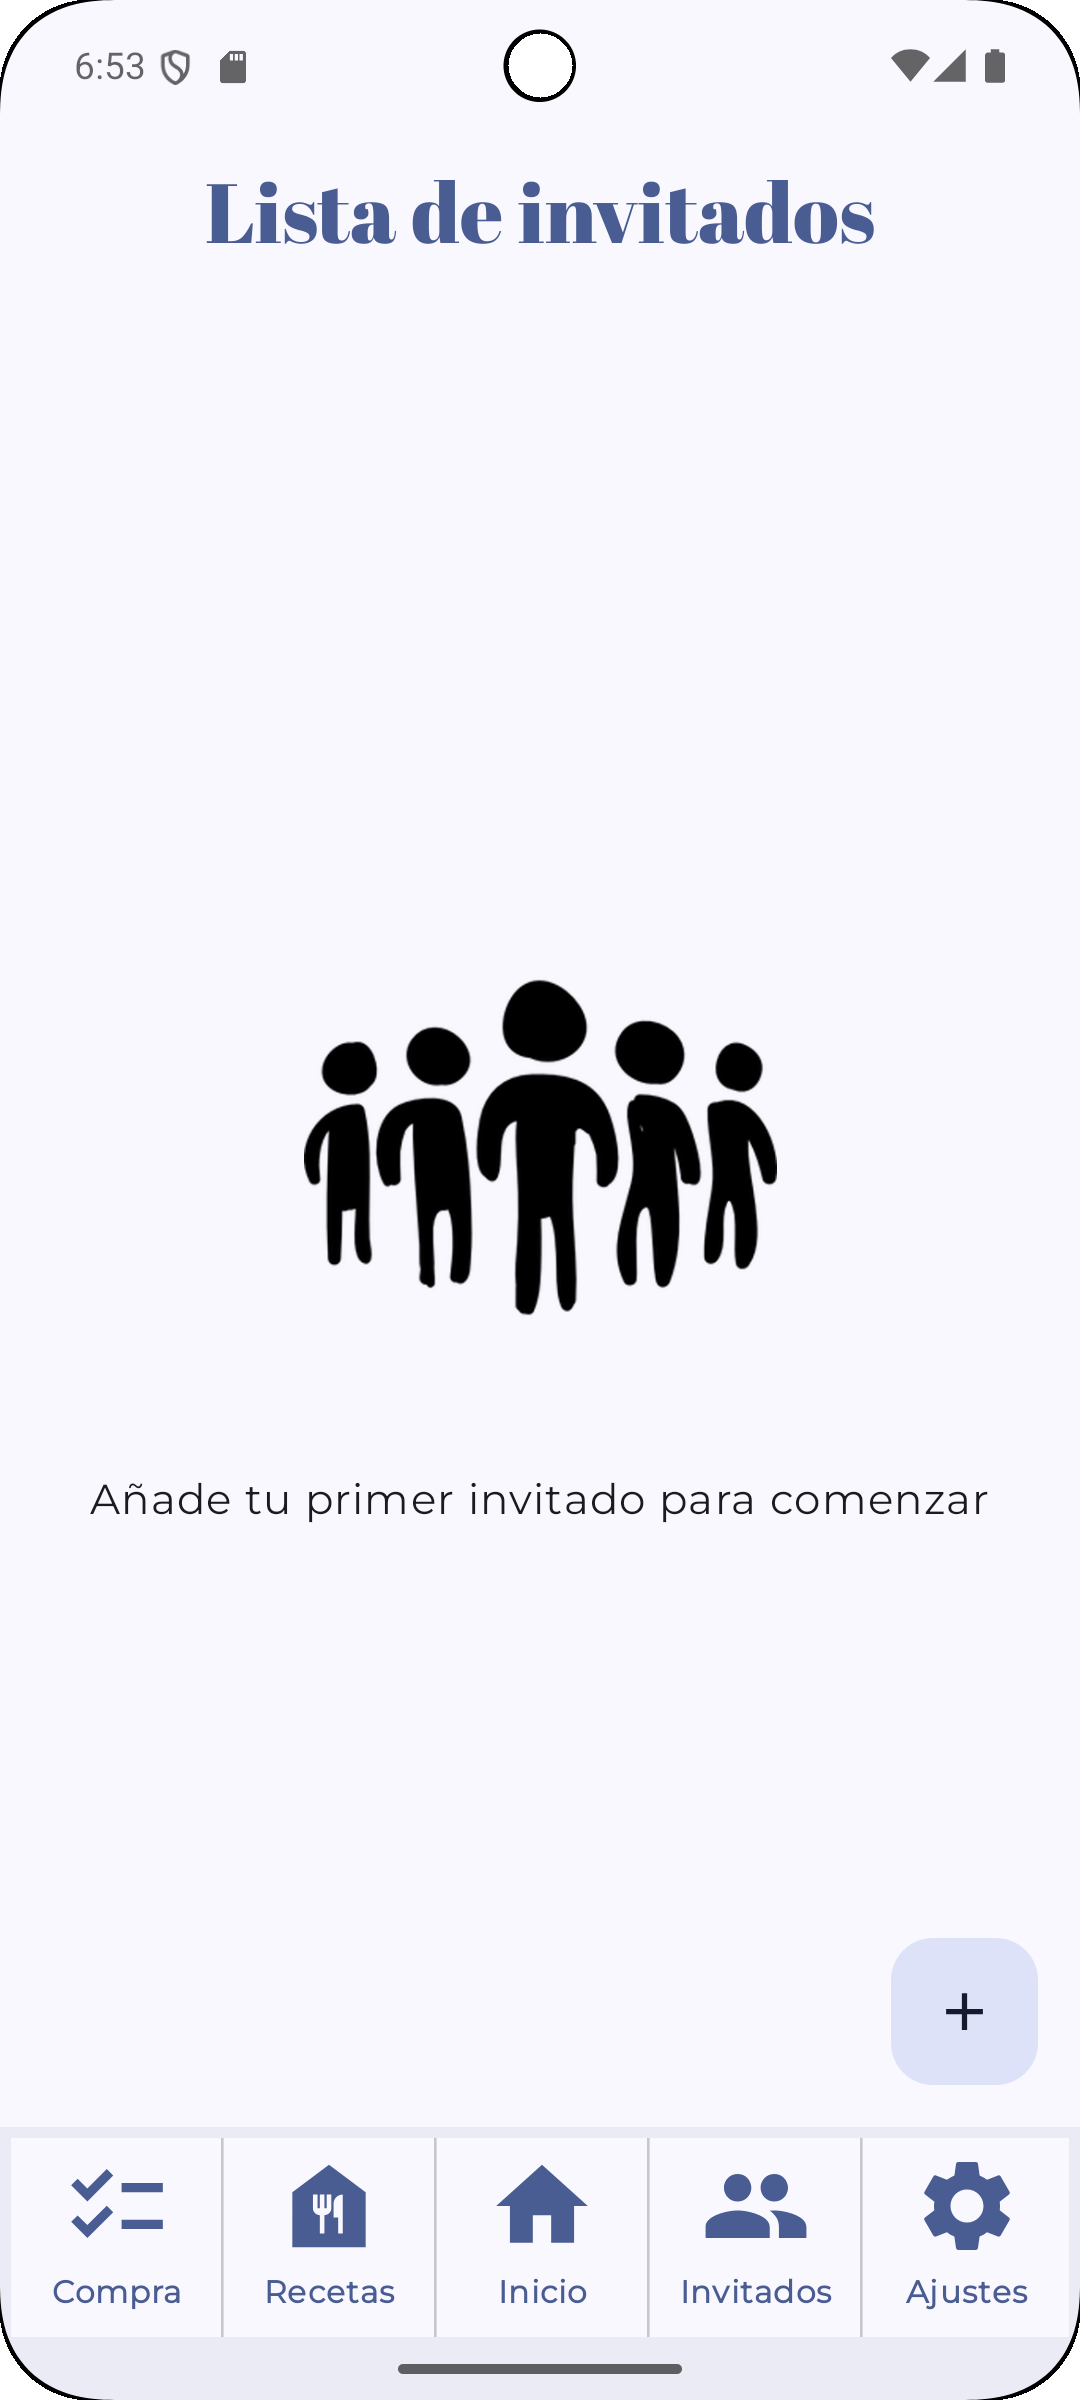
\includegraphics[width=\textwidth]{./img/manual/empty_guests.png}
      \caption{Pantalla de invitados vacía}
      \label{fig:guest-empty}
    \end{subfigure}
    \hfill
    \begin{subfigure}[b]{0.3\textwidth}
      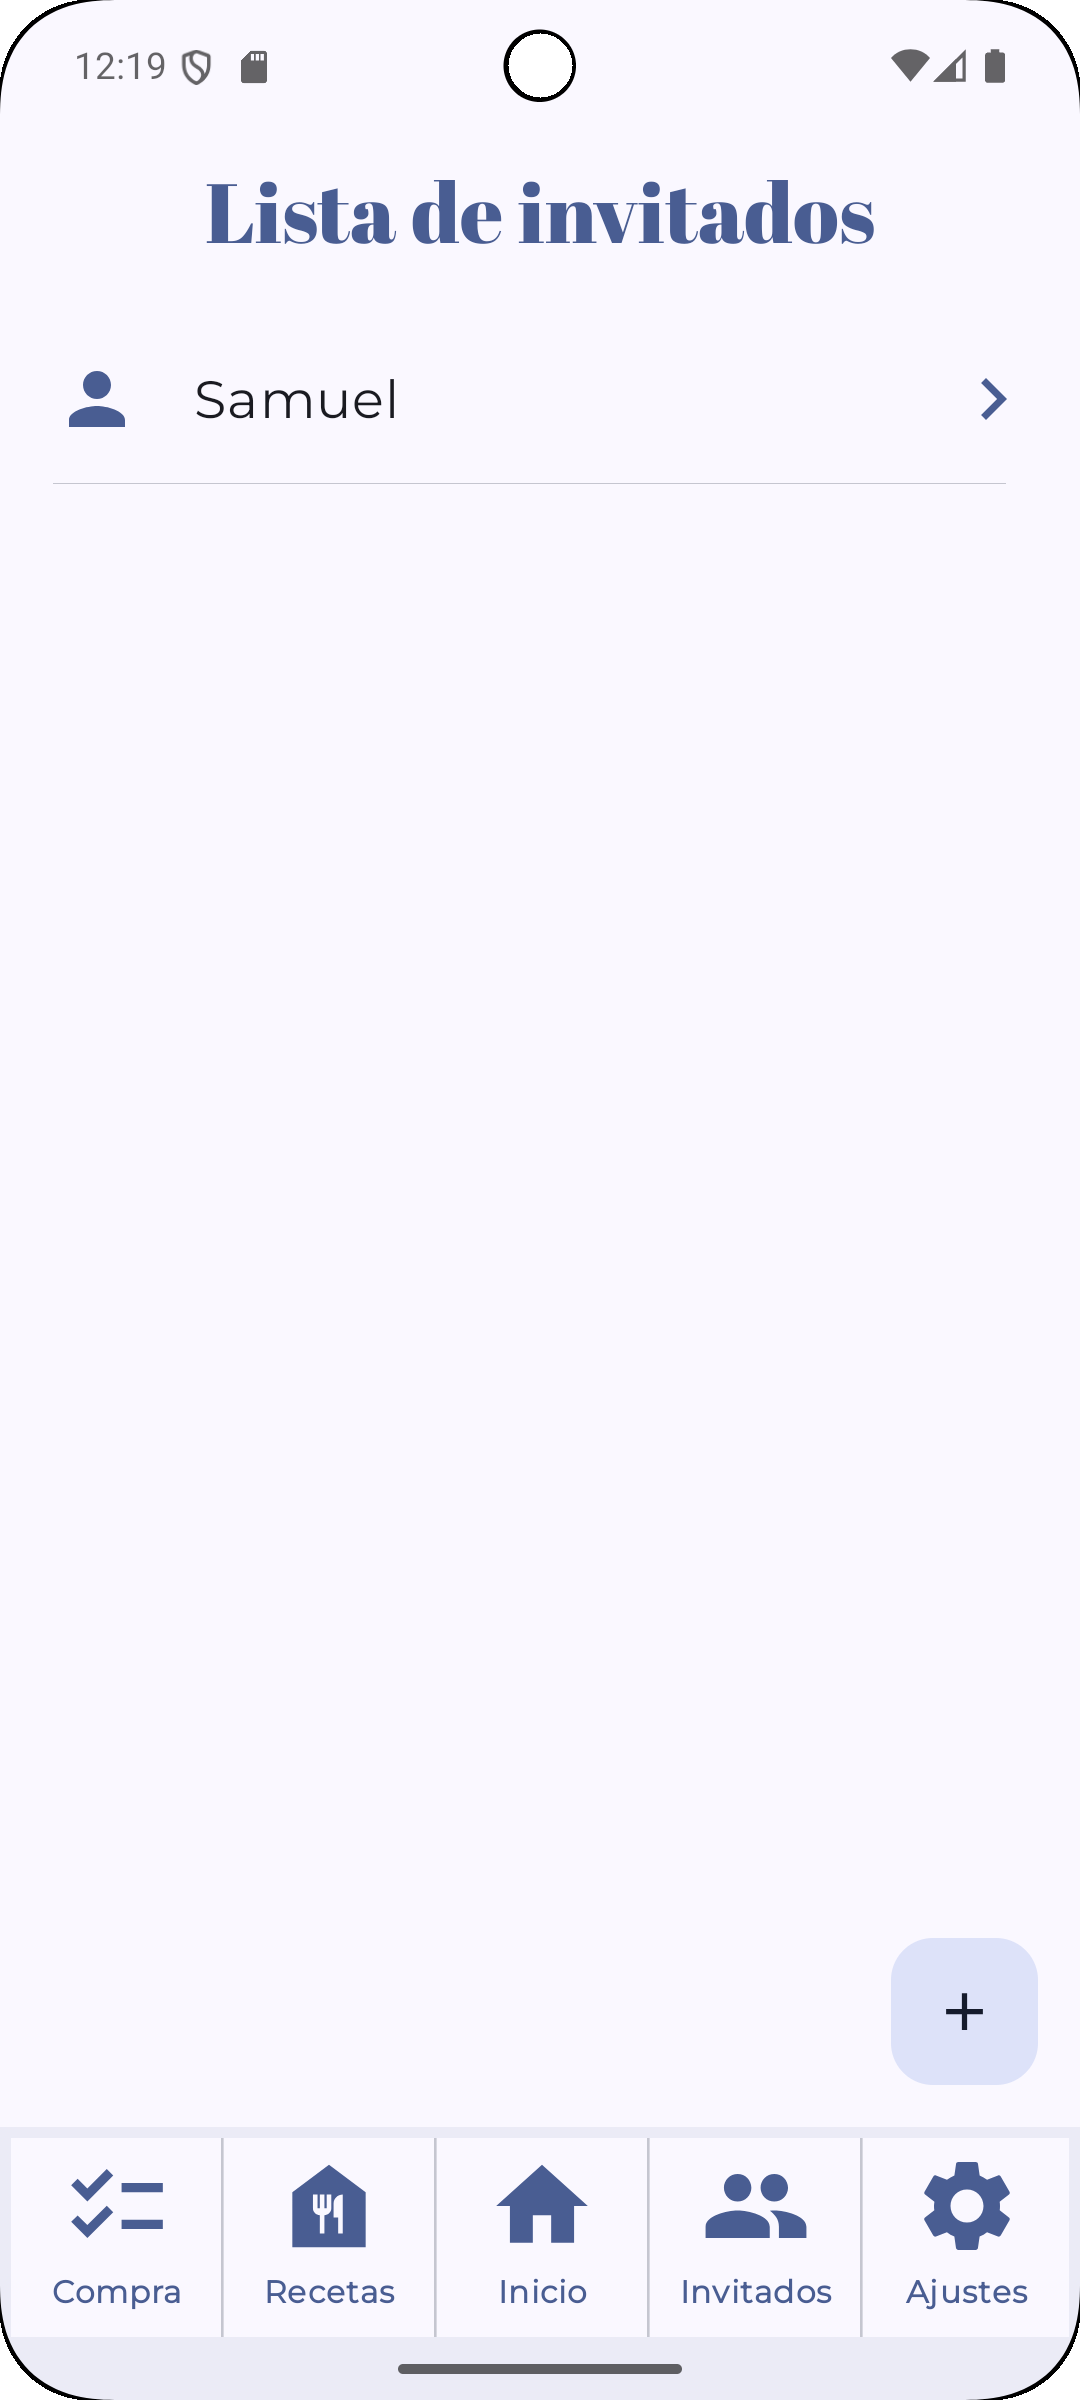
\includegraphics[width=\textwidth]{./img/manual/guests_not_empty.png}
      \caption{Pantalla de invitados}
      \label{fig:guest-not-empty}
    \end{subfigure}
    \hfill
    \begin{subfigure}[b]{0.3\textwidth}
      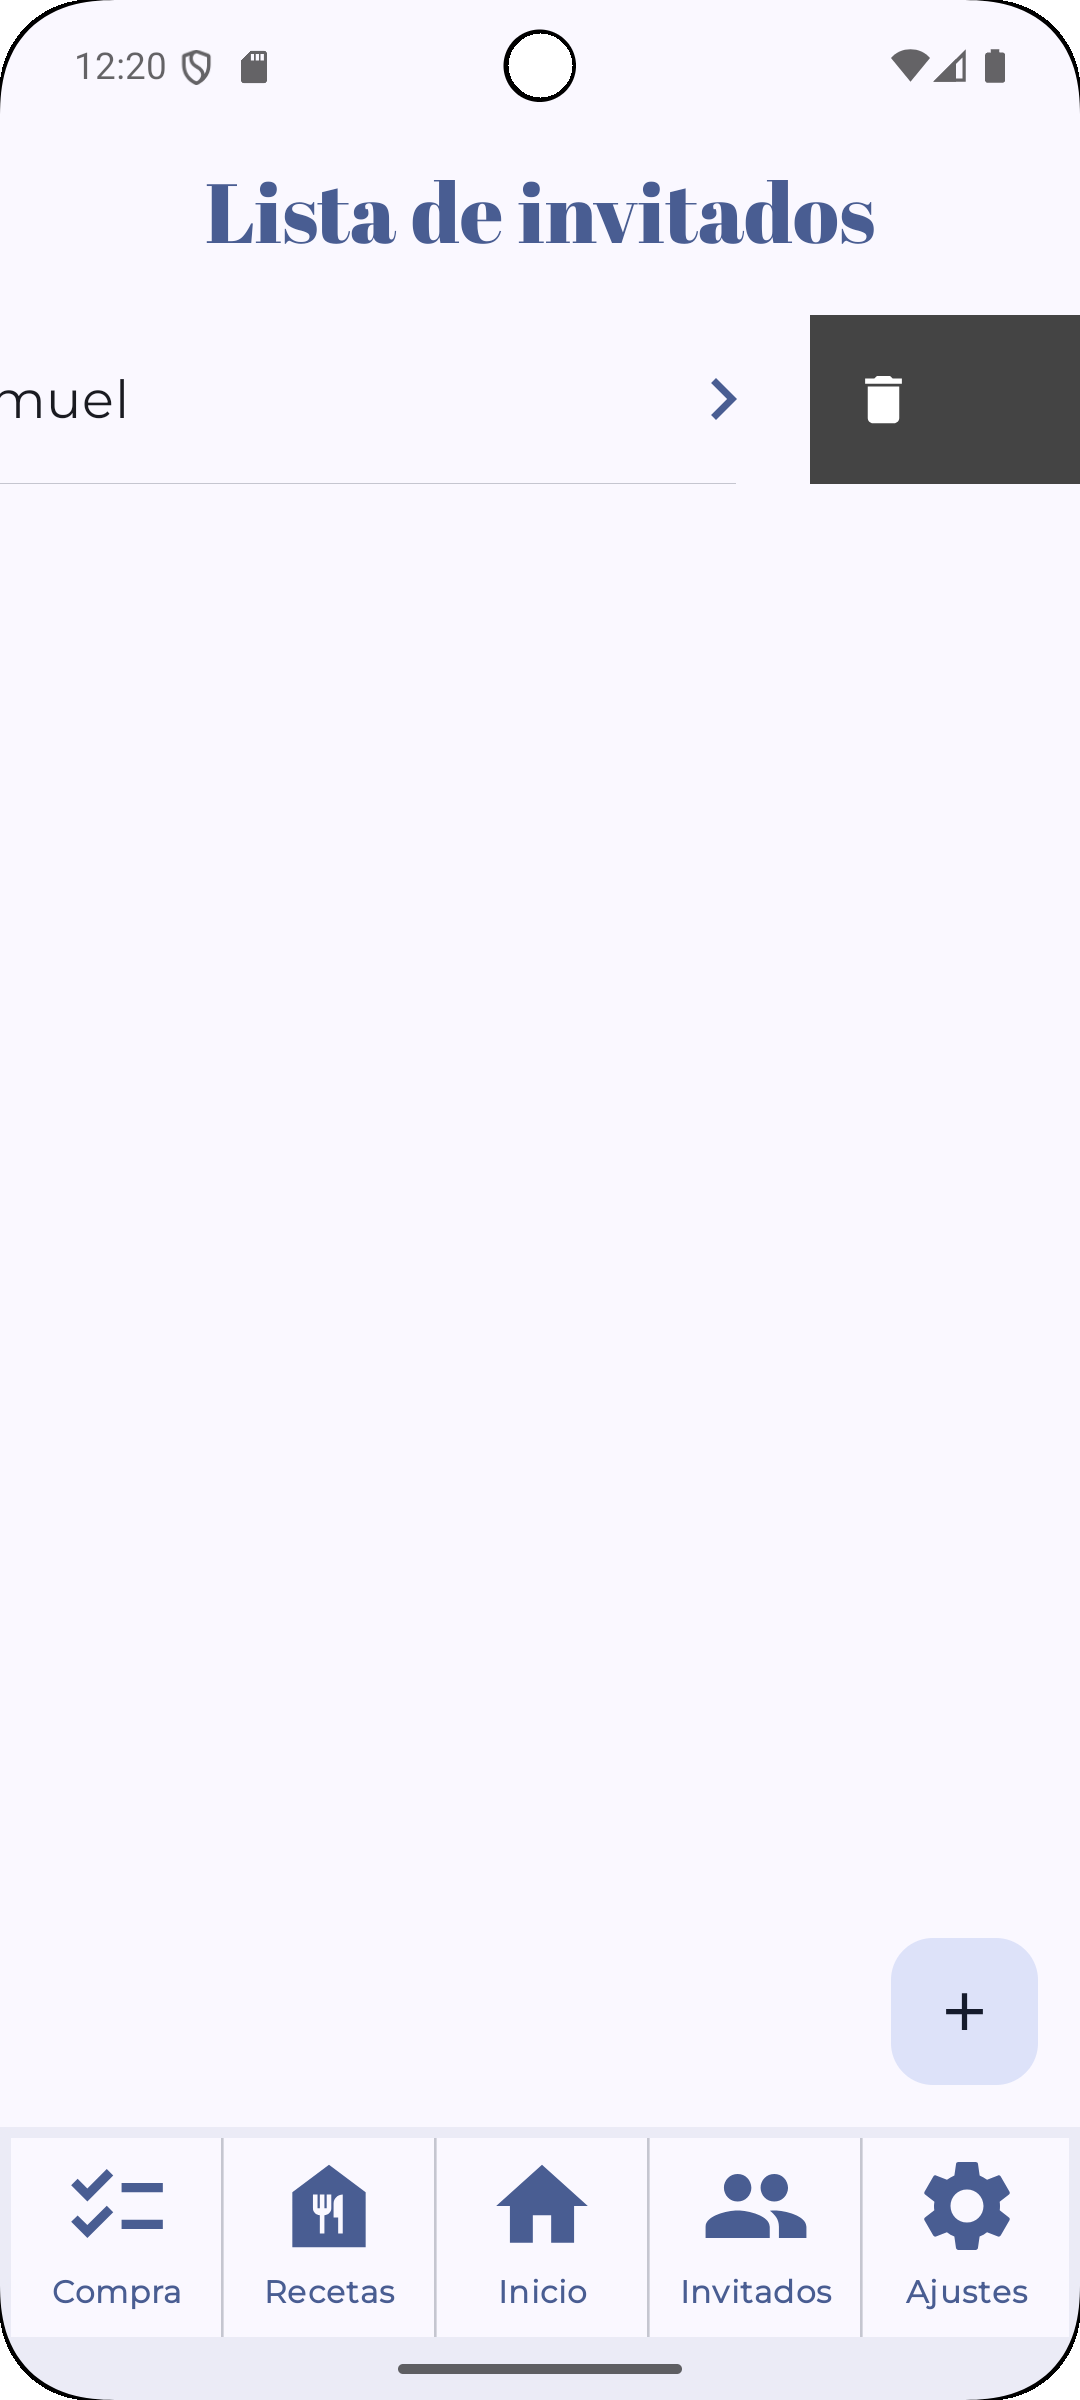
\includegraphics[width=\textwidth]{./img/manual/delete_guest.png}
      \caption{Eliminar invitado}
      \label{fig:delete-guest}
    \end{subfigure}

    \caption{Invitados}
    \label{fig:guests}
\end{figure}